\documentclass[14pt]{extarticle}

%%%% paramètres généraux
%%%% Pour avoir les accents et autre caractère français
\usepackage[french]{babel}
\usepackage[T1]{fontenc}
\usepackage[utf8]{inputenc}

%%%% Paquets utilisé
\usepackage{ifthen} % pour programmer avec des boucle et des conditions
%% Images/dessin
\usepackage{subcaption} % pour les légendes des figures
\usepackage{graphicx} % pour insérer des images
\usepackage[european, straightvoltages, RPvoltages]{circuitikz} % pour dessiner des circuits électrique
\usepackage{pdfpages} % pour inclure des fichiers pdf
\usepackage{wrapfig} % pour entourer les images par du texte 
\usepackage{chemfig} % pour dessiner des formules chimiques
\usepackage{fontawesome} % pour dessiner de jolies icônes
%% Mise en page
\usepackage{geometry} % définition des marges
\usepackage{dashundergaps} % pour avoir générer des textes à compléter
\usepackage{fancyhdr} % pour faire des en-tête
\usepackage[many]{tcolorbox} % pour faire de jolie boîtes colorée
\usepackage{enumitem} % pour pouvoir définir des listes personnalisées
\usepackage{hyperref} % pour insérer des liens
\usepackage{multicol} % pour avoir plusieurs colonnes côte-à-côte
\usepackage{listings} % pour insérer du code
%% Tableau
\usepackage{tabularray} % pour avoir de meilleurs tableaux
%% Math
\usepackage{amsmath} % symboles mathématiques
\usepackage{amssymb} % symboles mathématiques en gras
\usepackage{wasysym} % pour avoir des symbole d'intégrale
\usepackage{accents} % pour les notations mathématiques avec une barre
\usepackage{physics} % pour les dérivées, les bra, les kets, etc.
\usepackage{esvect} % pour faire de jolis vecteurs
\usepackage{siunitx} % pour avoir de jolie grandeurs avec des unités 
%% Décommenter pour avoir une police spéciale dysléxie (doit être compilé en XeTeX)
% \usepackage{fontspec}
% \setmainfont{OpenDyslexic}


%%%% Réglages de la taille des indentations et des sauts de paragraphes
\setlength{\parskip}{0cm}
\setlength{\parindent}{0cm}
\renewcommand{\baselinestretch}{1}
% réglage du niveau (sous-section) ou s'arrête la table des matières
\setcounter{tocdepth}{2}


%%%% Réglage de la géométrie des pages
\geometry{
  a4paper, % format
  left=1.3cm, right=1.3cm, % marge horizontale
  top=2.2cm, bottom=2.3cm % marge verticale
}


%%%% Réglage de chemfig
\setchemfig{
  atom sep=26pt,
  bond style={line width=1pt},
  angle increment=30
}


%%% Apparence (couleur) des liens
\hypersetup{
  colorlinks=true,
  linkcolor=black, % lien type table des matière
  citecolor=black, % citation
  filecolor=black, 
  urlcolor=blue!90!black % lien internet
}


%%%% Réglage de tikz (flèche et caractères)
\usetikzlibrary{babel}
\tikzset{>=latex}


%%%% Réglage des en-tête
\renewcommand{\headrulewidth}{0.4pt}
\setlength{\headheight}{22.50113pt}


%%%% Réglage de dashundergaps pour avoir des points et pas de numération
\dashundergapssetup{
  gap-numbers = false,
  gap-format = dot,
  gap-widen,
  gap-extend-percent
}


%%%% Réglage de siunit
\sisetup{
  locale = FR, % français
	 group-minimum-digits = 4, % groupage des chiffres par millier
  inter-unit-product = \ensuremath { { } \cdot { } } % point médian entre les unités
}
\AtBeginDocument{\RenewCommandCopy\qty\SI} % Pour "écraser" la commande \qty du package physics

%%%% quelques commandes
%%%%%%%%%%%%%%%%%%%%%%%%%%%%%%%%%%%%%%%%%%%%%%%%%%%%%%%%%%%%%%%%%%%%%%%%%%
%%%% quelque couleurs
\definecolor{vertSombre}  {RGB} {  0,  95,  17}
\definecolor{vertForet}   {RGB} {124, 179,  66}
%
\definecolor{jauneSombre} {RGB} {213, 145,   2}
\definecolor{orangeSombre}{RGB} {174,  82,   0}
\definecolor{cyanSombre}  {RGB} {  0, 140, 128}
\definecolor{bleuPale}    {RGB} { 39,  76, 167}
%
\definecolor{jauneClair} {RGB} {218, 173,   0}
\definecolor{rougeSombre}{RGB} {148,  31,   0}
\definecolor{rougeClair} {RGB} {224,  39,  34}

%%% quelques couleurs dérivées des couleurs choisie
\newcommand{\couleurPrimSombre}{couleurPrim!60!black}

%%%% rectangle coloré
\NewDocumentCommand{\rectangle}{O{couleurPrim} m m}{%
  \shorthandoff{;}
  \tikz \node (rect) [draw, fill, color=#1,
              minimum width=#2,
              minimum height=#3] {};
  \shorthandon{;}
}


%%%%%%%%%%%%%%%%%%%%%%%%%%%%%%%%%%%%%%%%%%%%%%%%%%%%%%%%%%%%%%%%%%%%%%%%%%%
%%%% une simple boite vide
\newtcolorbox{boite}[1][]{
  breakable, enhanced jigsaw, % pour s'étendre sur plusieurs pages
  arc = 0mm, % les lignes de la boites sont droites
  colback = white, colframe = black, % fond blanc et traits noirs
  #1
}

%%%% boite colorée
\newtcolorbox{boiteColoree}[1][]{
  breakable, enhanced jigsaw, % pour s'étendre sur plusieurs pages
  arc = 2mm, % les lignes de la boites sont droites
  colback = couleurPrim, colframe = white, % fond et traits colorés
  coltext = white,
  #1
}

%%%% document
\newcounter{documentNum}
\newtcolorbox{doc}[3][]{
  before title = {\refstepcounter{documentNum}},
  breakable, enhanced jigsaw, % pour s'étendre sur plusieurs pages
  colback = white, % fond blanc
  colframe = couleurPrim!25!black, % couleur de la boite
  coltitle = black, % couleur du titre
  boxrule = 0.5mm, arc = 0.5mm, % largeur et arrondi des traits de la boite
  titlerule = 0mm, top = 0mm, % pour ne pas avoir de séparation titre/boite
  colbacktitle = white, % fond pour le titre blanc
  fonttitle = \bfseries\sffamily,
  title = {Document \arabic{documentNum} -- #2\strut \label{#3}},
  #1
}

%%%% Passage important à connaître
\newtcolorbox{encart}[1][]{
  breakable, enhanced jigsaw, % pour s'étendre sur plusieurs pages
  frame hidden, sharp corners, boxrule = 0mm, % pas de contours
  colback = couleurPrim!10, % fond
  borderline west={4pt}{0pt}{couleurPrim}, % barre gauche
  #1
}

%%%% Boite de correction
\newtcolorbox{boiteCorrection}[1][]{
  breakable, enhanced jigsaw, % pour s'étendre sur plusieurs pages
  frame hidden, sharp corners, boxrule = 0mm, % pas de contours
  colback = couleurPrim!10, % fond
  #1
}

%%%% contexte
\newtcolorbox{contexte}[1][]{
  breakable, enhanced jigsaw, % pour s'étendre sur plusieurs pages
  boxrule = 3pt, sharp corners, % contours droits
  colframe = couleurPrim, % couleur des contours
  colback = couleurPrim!5, % fond
  title = {Contexte :}, % titre
  colbacktitle = couleurPrim!5, % couleur du fond du titre
  fonttitle = \bfseries\sffamily, coltitle = black, %
  titlerule = 0mm, top = 0mm, % pour ne pas avoir de séparation titre/boite
  detach title, before upper={\vspace{2pt}\hspace{-8pt}\tcbtitle\;},
  #1
}

%%%% Pour les objectifs
\newtcolorbox{boiteObjectifs}[2][]{
  empty, % pas de boite automatique
  attach boxed title to top left = {yshift=-2.5mm}, % position
  boxed title style = {empty, size = small, top = 1mm, bottom = 0.5mm},
  frame code = { % tracé de la boite
    \path (title.east |- frame.north) coordinate (aux);
    \path [draw=couleurPrim, line width = 3pt]
    (frame.west) |- ([xshift=-4mm] title.north east)
    to[out=0, in=180] ([xshift=10mm] aux) -| % définit la courbe
    (frame.east) |- (frame.south) -| cycle; % trace la boite
  },
  coltitle = black, % couleur du titre
  fonttitle = \bfseries\sffamily, % police du titre
  title = {#2},
  #1 
}
\newenvironment{objectifs}{
  \begin{boiteObjectifs}{Objectifs de la séance :}
    \begin{listeObjectifs}
}{
    \end{listeObjectifs}
  \end{boiteObjectifs}
}

%%%% Espace pour un coup de pouce
\newcounter{coupDePouceNum}
\newtcolorbox{coupDePouce}[1][]{
  before title = {\refstepcounter{coupDePouceNum}},
  breakable, enhanced jigsaw, % pour s'étendre sur plusieurs pages
  arc = 0mm, % les lignes de la boites sont droites
  colback = white, colframe = black, % fond blanc et traits noirs
  fonttitle = \bfseries, coltitle = black, % couleur et police du titre
  titlerule = 0mm, top = 0mm, % pour ne pas avoir de séparation titre/boite
  colbacktitle = white, % fond pour le titre blanc
  title = {
    \textcolor{couleurPrim}{\faThumbsUp}
    Coup de pouce \arabic{coupDePouceNum} :
    \flushright \vspace*{-26pt}\faSquareO
  },
  #1
}

%%%% Espace pour une appréciation
\newcommand{\appreciation}[1]{
  \pasCorrection{
    \begin{boite}
      \vspace*{-4pt}
      \sousTitre{Appréciation et remarques}
      
      \vspace*{#1 cm}
      \phantom{b}
    \end{boite}
  }
}

%%%% Espace fiche TP
\newtcolorbox{boiteMateriel}[2][]{
  colback = white, colframe = black, % fond blanc et traits noirs
  coltitle = white, % couleur du titre
  boxrule = 0.5mm, arc = 0.5mm, % largeur et arrondi des traits de la boite
  titlerule = 0mm, top = 0mm, % pour ne pas avoir de séparation titre/boite
  colbacktitle = couleurPrim, % fond pour le titre blanc
  fonttitle = \bfseries\sffamily, % type de titre
  title = {\centering \large #2}, % titre
  #1
}

%%%%%%%%%%%%%%%%%%%%%%%%%%%%%%%%%%%%%%%%%%%%%%%%%%%%%%%%%%%%%%%%%%%%%%%%%%
%%%% pagination et sections
\newcommand{\titre}[1]{
  \begin{center}
    \textsf{\bfseries \Large #1}
  \end{center}
}
\newcommand{\sousTitre}[1]{
  \textsf{\bfseries #1}
}
\newcommand{\pasDePagination}{
  \thispagestyle{empty}
}
\newcommand{\feuilleBlanche}{
  \newpage
  \phantom{b}
  \pasDePagination
}
    

%%%% activité ou TP
\newcounter{activiteNum}
\newcommand{\titreActi}[2]{
  \refstepcounter{activiteNum}
  \titre{#1 \arabic{section}.\arabic{activiteNum} -- #2}
}
\newcommand{\titreTP}[1]{
  \titreActi{TP}{#1}
  % \titreActi{Activité expérimentale}{#1}
}
\newcommand{\titreActivite}[1]{
  \titreActi{Activité}{#1}
}
\NewDocumentCommand{\titreEvaluation}{o m}{
  \IfNoValueTF {#1}{
    \titre{Évaluation \arabic{section} -- #2}
  }{
    \titre{Évaluation #1 -- #2}
  }
  % reset du numéro de page et d'exercices
  \setcounter{page}{1}
  \numeroActivite{1}
}
\newcounter{exerciceNum}
\newcommand{\exercice}[1]{
  \refstepcounter{exerciceNum}
  \sousTitre{\large Exercice \arabic{exerciceNum} : #1}
  % reset des numéros de questions
  \setcounter{questionNum}{0}
  \setcounter{documentNum}{0}
}


%%%% chapitre, section et sous-section
\newcommand{\titreChapitre}[1]{
  \titre{Chapitre \arabic{section} : #1}
}
\newcommand{\titrePartie}[1]{
  \vspace*{24pt}
  \refstepcounter{subsection}
  \rectangle{40pt}{1pt}
  \sousTitre{\Large \Roman{subsection} -- #1}
  \rectangle{40pt}{1pt}
  \vspace*{10pt}
}
\newcounter{sousSectionNum}
\newcommand{\titreSection}[1]{
  \vspace*{16pt}
  \refstepcounter{subsubsection}
  \setcounter{sousSectionNum}{0}
  \rectangle{30pt}{4pt}
  \sousTitre{\large \arabic{subsubsection} -- #1}
  \vspace*{10pt}
}
\newcommand{\titreSousSection}[1]{
  \vspace*{12pt}
  \refstepcounter{sousSectionNum}
  \sousTitre{\Alph{sousSectionNum} -- #1}
  \vspace*{8pt}
}

%%%% fixe le numéro de l'activité
\newcommand{\numeroActivite}[1]{
  % fixe les compteurs LaTeX
  \setcounter{page}{1}
  \setcounter{subsection}{0}
  \setcounter{subsubsection}{0}
  \setcounter{figure}{0}
  % fixe les compteurs internes
  \setcounter{qcmNum}{0}
  \setcounter{documentNum}{0}
  \setcounter{questionNum}{0}
  \setcounter{coupDePouceNum}{0}
  \setcounter{sousSectionNum}{0}
  \setcounter{activiteNum}{#1 - 1}
}
% fixe le numéro de partie (#1) et le numéro de la page (#2)
\newcommand{\numeroPartieCours}[2]{
  \newpage
  \setcounter{subsection}{#1 - 1}
  \setcounter{page}{#2}
}

%%%% lignes
\newcommand{\ligne}{
  \par\noindent\rule{\textwidth}{0.4pt}
}
\newcommand{\lignePointillee}[1]{
  \makebox[#1\linewidth]{\dotfill}
}


%%%%%%%%%%%%%%%%%%%%%%%%%%%%%%%%%%%%%%%%%%%%%%%%%%%%%%%%%%%%%%%%%%%%%%%%%%
%%%% Paramètre par défaut pour l'en-tête
\newcommand{\annee}{Réglez avec \textbackslash renewcommand\{\textbackslash annee\}\{2023 -- 2024\}}
\newcommand{\classe}{Réglez avec \textbackslash renewcommand\{\textbackslash classe\}\{Seconde\}}
\newcommand{\etablissement}{Réglez avec \textbackslash renewcommand\{\textbackslash etablissement\}\{Lycée\}}

%%%% en-tête
\newcommand{\teteGauche}[2]{
  \lhead{
    \textbf{\footnotesize #1}
    \newline
    \footnotesize #2
  }
}
\newcommand{\teteDroite}[2]{
  \rhead{
    \hfill \textbf{\footnotesize #1}
    \newline \hfill
    \footnotesize #2
  }
}
\newcommand{\enTete}[3]{
  \pagestyle{fancy}
  \setcounter{section}{#3}
  \setcounter{subsection}{0}
  \setcounter{sousSectionNum}{0}
  \teteGauche{\etablissement{}}{Chapitre \arabic{section} -- #1} % left header
  \chead{} % central header
  \teteDroite{\annee{}}{#2} % right header
}


%%%%%%%%%%%%%%%%%%%%%%%%%%%%%%%%%%%%%%%%%%%%%%%%%%%%%%%%%%%%%%%%%%%%%%%%%%
%%%% exercice
% définit un booléen pour entrer ou sortir du mode correction
\newboolean{modeProf}
\setboolean{modeProf}{false}
\newcommand{\modeCorrection}{
  \setboolean{modeProf}{true}
  \TeacherModeOn
}

% Pour afficher le numéro d'une question avec choix du compteur
\NewDocumentCommand{\numeroQuestion}{O{questionNum} O{16}}{
  \refstepcounter{#1}
  \setcounter{sousQuestionNum}{0}
  \vspace*{2pt}
  \ifnum \thequestionNum > 9
    \hspace{6 pt}
  \else
    \hspace{#2 pt}
  \fi
  \textcolor{couleurSec}{
    \textbf{\arabic{#1}} {\small\faMinus}
  }
}

\newcommand{\numeroSousQuestion}{
  \refstepcounter{sousQuestionNum}
  \hspace{16 pt}
  \textcolor{couleurSec}{
    \textbf{\arabic{questionNum}.\arabic{sousQuestionNum}.}
  }
}


% trace des lignes pointillées pour répondre aux questions
% \lignessDeReponse* complète la ligne actuelle par des pointillées
% \lignesDeReponse commence à la ligne suivante
\newcounter{ligneNum}
\NewDocumentCommand{\lignesDeReponse}{s m}{
  % Trace la fin de la ligne, ou pas
  \IfBooleanTF{#1}{ % Version *
    \espaceReponse \dotfill\phantom{bb}
    \ifnum #2 < 1
      \newline
    \fi
  }{}
  % Trace le bon nombre de lignes
  \setcounter{ligneNum}{-1}
  \loop
    \stepcounter{ligneNum}
    \ifnum \value{ligneNum} < #2
      \\[8pt] \lignePointillee{0.98}
  \repeat
  \vspace*{1pt}
}


% définit une commande pour afficher une question 
% #1 : question
% #2 : réponse
% #3 : nombres de lignes pour répondre
\newcounter{questionNum}
\newcounter{sousQuestionNum}
\newcommand{\question}[3]{
  \numeroQuestion \!#1
  % pointille ou correction
  \ifthenelse {\boolean{modeProf}} { % prof
    \begin{boiteCorrection}
      #2
    \end{boiteCorrection}
  }{ % eleve
    \lignesDeReponse{#3}
  }
}

% Affiche le contenu en mode correction
\newcommand{\correction}[1]{
  \ifthenelse {\boolean{modeProf}} { % correction
    #1
  }{}
}

% Affiche le contenu si on est pas en mode correction
\newcommand{\pasCorrection}[1]{
  \ifthenelse{\boolean{modeProf}} {}{ % pas correction
    #1
  }
}

% Point associé à une question
\newcommand{\points}[1]{
  \marginnote{#1}
}


% sous questions
\newcommand{\sousQuestion}[2]{
  \hspace{16pt}
  \textcolor{couleurSec}{\textbullet} #1
  
  \vspace*{8pt}
  \reponse{#2}
}

% question QCM
\newcommand{\QCM}[2]{
  \numeroQuestion[qcmNum][0] #1
  \begin{qcm}
    #2
  \end{qcm}
}

% À ajouter devant la bonne réponse dans un qcm
\newcounter{qcmNum}
\newcommand{\reponseQCM}{
  \correction{
    \hspace*{-15pt}$\checkmark$\hspace*{-12pt}
  } % Note : trace une croix à la bonne position
}

%%%% Pour afficher les compétences
\newcommand{\competence}[1]{
  ~{\footnotesize\textit{(#1)}}
}

%%%% Espace pour indiquer nom, prénom et classe
\newcommand{\nomPrenomClasse}{
  \pasCorrection{
    \vspace*{-24pt}
    Nom : \lignePointillee{0.3}
    Prénom : \lignePointillee{0.3}
    Classe : \dotfill
  }
}
\newcommand{\nomPrenom}{
  \pasCorrection{
    \vspace*{-24pt}
    Nom : \lignePointillee{0.3}
    Prénom : \lignePointillee{0.3}
  }
}


%%%%%%%%%%%%%%%%%%%%%%%%%%%%%%%%%%%%%%%%%%%%%%%%%%%%%%%%%%%%%%%%%%%%%%%%%%
% texte à trou avec option pour régler la largeur
\NewDocumentCommand{\texteTrou}{o +m}{
  \ifthenelse {\boolean{modeProf}}{ % prof
    \important[black]{#2}
  }{ % élève
    \IfValueTF{#1}{ % Si la largeur est réglée, on utilise des lignes
      \espaceReponse
      \lignePointillee{#1}
      \hspace*{-12pt}
    }{ % Sinon on utilise dash undergap pour la version automatique
      \espaceReponse \hspace*{0.1pt}
      \gap{#2}
    }
  }
}

% texte à trou avec option pour laisser plusieurs lignes
\NewDocumentCommand{\texteTrouLignes}{O{0} +m}{
  \ifthenelse {\boolean{modeProf}} {% prof
    \important[black]{#2}
  }{% élève
    \lignesDeReponse*{#1}
  }
}

% espace vertical pour la réponse
\newcommand{\espaceReponse}{
  \phantom{$\dfrac{1}{1}$} % espace vertical
  \hspace*{-38pt} \phantom{b} % ajuste l'espace horizontal
}


%%%%%%%%%%%%%%%%%%%%%%%%%%%%%%%%%%%%%%%%%%%%%%%%%%%%%%%%%%%%%%%%%%%%%%%%%%
%%%% Pour choisir parmi deux sujets
\newboolean{sujetA}
\setboolean{sujetA}{true}
\newcommand{\sujetB}{
  \setboolean{sujetA}{false}
}
\newcommand{\sujetA}{
  \setboolean{sujetA}{true}
}

%%%% Pour faire plusieurs sujets en parallèle
\newcommand{\variationSujet}[2]{
  \hspace*{-6pt}
  \ifthenelse {\boolean{sujetA}}{#1}{#2}
  \hspace*{-6pt}
}


%%%%%%%%%%%%%%%%%%%%%%%%%%%%%%%%%%%%%%%%%%%%%%%%%%%%%%%%%%%%%%%%%%%%%%%%%%
%%%% Tableau générique avec la première ligne bleue
\NewDocumentEnvironment{tableau}{m}{
  \begin{center}
    \begin{tblr}{
      hlines,
      colspec = #1,
      row{1} = {couleurPrim!20},
    }
}{
    \end{tblr}
  \end{center}
}

%%%% Tableau de competence
\newenvironment{tableauCompetences}{
  \centering
  \begin{tblr}{
    colspec = {| c | X[l] | c | c | c | c |},
    rows = {m}, hlines,
    row{1} = {couleurPrim!20}
  }
    \textbf{Compétences} & \centering \textbf{Items} 
    & \textbf{D} & \textbf{C} & \textbf{B} & \textbf{A} \\
}{
  \end{tblr}
}

%%%% Tableau de connaissances sans exercices
\newenvironment{tableauConnaissances}{
  \centering
  \begin{tblr}{
    colspec = {Q[t,wd=0.7\textwidth] c c c},
    rows = {m}, hlines, vlines,
    column{4} = {0.2},
    row{1} = {couleurPrim!20, c}
  }
    \textbf{Connaissances et capacités exigibles} & \ok & \pasOk & \textbf{En classe} \\
}{ 
  \end{tblr}
}


%%%% Alignement dans un tableau
\newcommand{\vAligne}[1]{
  \strut \\ \vspace*{#1}
}


%%%%%%%%%%%%%%%%%%%%%%%%%%%%%%%%%%%%%%%%%%%%%%%%%%%%%%%%%%%%%%%%%%%%%%%%%%
%%%% symboles : chevron, flèche, attention, etc.
\NewDocumentCommand{\chevron}{O{couleurPrim}}{
  \textcolor{#1}{\small \faChevronRight}
}
%
\NewDocumentCommand{\fleche}{O{couleurPrim}}{
  \textcolor{#1}{\faCaretRight}
}
%
\NewDocumentCommand{\attention}{O{couleurPrim}}{
  \textcolor{#1}{\faExclamationTriangle}
}
%
\NewDocumentCommand{\flecheLongue}{O{couleurPrim}}{
  \textcolor{#1}{\faLongArrowRight}
}
%
\NewDocumentCommand{\ok}{O{couleurPrim}}{
  \textcolor{#1}{\faCheckCircle}
}
%
\NewDocumentCommand{\pasOk}{O{couleurPrim}}{
  \textcolor{#1}{\faTimesCircle}
}
%
\NewDocumentCommand{\pointCyan}{O{couleurPrim}}{
  \textcolor{#1}{\textbullet}
}
%
\NewDocumentCommand{\mesure}{O{couleurPrim}}{
  \hspace{15pt}
  %\numeroQuestion
  \textcolor{couleurSec}{\faWrench\faFlask}
}
% pictogramme sécurité
\newcommand{\picto}[2]{
  \image{#1}{images/pictogrammes/picto_#2}
}
% Nombre dans un cercle
\newcommand*\nombreCercle[1]{
  % \tikz[baseline=(char.base)]{
  %   \node [shape=circle, draw filled, inner sep=1.2pt, color=couleurSec!20] (char) {\textcolor{black}{#1};
  % }
  \important[couleurSec]{#1}
}
% Pour légender une image
\newcommand{\legende}[1]{
  \textcolor{couleurPrim}{\faArrowUp} \; #1
}

%%%%%%%%%%%%%%%%%%%%%%%%%%%%%%%%%%%%%%%%%%%%%%%%%%%%%%%%%%%%%%%%%%%%%%%%%%
%%%% emphase
\newcommand{\emphase}[1]{
  \textcolor{couleurSec}{\textsf{\bfseries \large #1}}
}
%
\NewDocumentCommand{\important}{O{couleurSec!75!black} m}{
  \!\textcolor{#1}{\textsf{\bfseries #2}}\!\!
}
%
\newcommand{\exemple}{
  \flecheLongue \textit{Exemple :}
}
\newcommand{\exemples}{
  \flecheLongue \textit{Exemples :}
}
%
\newcounter{compteAppelProf}
\newcommand{\appelProf}{
  \refstepcounter{compteAppelProf}
  \hspace{24pt} \faHandPaperO \hspace{2pt}
  \textbf{Appel n$^\circ$ \arabic{compteAppelProf} :}
}

%
\newcommand{\extrait}[2]{
  « #1 »
  
  \vspace*{-12pt}
  \begin{flushright}
    \textit{#2}
  \end{flushright}
  \vspace*{-12pt}
}


%%%% image
\newcommand{\image}[2]{
  \includegraphics[width=#1\linewidth]{#2}
}

%%%% qr code en insert sur la droite
\NewDocumentCommand{\QRCode}{o m}{
  \IfNoValueTF{#1} {
    \begin{wrapfigure}{r}{0.1\linewidth}
      \vspace*{-16pt}
      \qrcode{#2}
    \end{wrapfigure}
  }{
    \begin{wrapfigure}[#1]{r}{0.1\linewidth}
      \vspace*{-16pt}
      \qrcode{#2}
    \end{wrapfigure}
  }
}


%%%%%%%%%%%%%%%%%%%%%%%%%%%%%%%%%%%%%%%%%%%%%%%%%%%%%%%%%%%%%%%%%%%%%%%%%%
%%%% qcm
\newlist{qcm}{itemize}{2}
\setlist[qcm]{label=$\square$, leftmargin=2cm}

%%%% liste d'objectif
\newlist{listeObjectifs}{itemize}{2}
\setlist[listeObjectifs]{label = \chevron}

%%%% protocole
\newlist{protocole}{itemize}{2}
\setlist[protocole]{label = {\footnotesize \fleche[couleurSec]}}

%%%% liste de points
\newlist{listePoints}{itemize}{2}
\setlist[listePoints]{label = \pointCyan}

%%%% liste tirets
\newlist{listeTirets}{itemize}{2}
\setlist[listeTirets]{label = \textcolor{couleurPrim}{\small\faMinus}}

%%%% liste avec des flèches
\newlist{listeFleche}{itemize}{2}
\setlist[listeFleche]{label = \textbf{\flecheLongue}}

%%%% jeu de données
\newenvironment{donnees}{
  
  \textbf{Données :}
  \vspace*{-8pt}
  \begin{multicols}{2}
    \begin{listeTirets}
}{
    \end{listeTirets}
  \end{multicols}
}

%%%% problematique
\newcommand{\problematique}[1]{
  \hspace{8pt}
  \flecheLongue
  \textbf{#1}
}

%%%% liste avec chiffre
\newlist{enumeration}{enumerate}{2}
\setlist[enumeration]{label = \textcolor{\couleurPrimSombre}{\textbf{\arabic*.}} }


%%%%%%%%%%%%%%%%%%%%%%%%%%%%%%%%%%%%%%%%%%%%%%%%%%%%%%%%%%%%%%%%%%%%%%%%%%
%%%% Séparation de la page en blocs
\newcommand{\separationTroisBlocs}[3]{
  \begin{minipage}[T]{0.3\linewidth}
    #1
  \end{minipage}
  ~
  \begin{minipage}[T]{0.3\linewidth}
    #2
  \end{minipage}
  ~
  \begin{minipage}[T]{0.3\linewidth}
    #3
  \end{minipage}
}
%%%% Separation en deux blocs
\NewDocumentCommand{\separationBlocs}{+m O{0.48} +m O{0.48}}{
  \begin{minipage}[T]{#2\linewidth}
    #1
  \end{minipage}
  \hfill
  \begin{minipage}[T]{#4\linewidth}
    #3
  \end{minipage}
}


%%%%%%%%%%%%%%%%%%%%%%%%%%%%%%%%%%%%%%%%%%%%%%%%%%%%%%%%%%%%%%%%%%%%%%%%%%
%% nombre algébrique, réaction
\newcommand{\algebrique}[1]{
  \overline{\mathrm{#1}}
}
\newcommand{\reaction}{
  \!\!\schemestart \arrow(.mid east--.mid west){->}[, 0.9, ultra thick] \schemestop\!\!
}

%% Pour simplifier l'écriture des formules brutes
\newcommand{\bruteCHO}[3]{
  \chemfig{C_{#1} H_{#2} O_{#3}}
}

%% pour les masse molaire et atomique
\newcommand{\masseMol}[1]{
  M(\chemfig{#1})
  % M_{\chemfig{#1}}
}
\newcommand{\masseAtom}[1]{
  m(\chemfig{#1})
  % m_{\chemfig{#1}}
}


%% Unités
\DeclareSIUnit{\dioptre}{\text{$\delta$}}
\DeclareSIUnit{\dornic}{\text{\textdegree D}}
\DeclareSIUnit{\ppm}{\text{ppm}}
\DeclareSIUnit{\COeq}{\text{kgCO$_{2}$e}}
\DeclareSIUnit{\jour}{\text{jour}}
% \DeclareSIUnit{}{\text{}}


%% atome ou isotope #1: Z, #2: A, #3: X
\makeatletter
\newcommand{\isotope}[3]{%
   \settowidth\@tempdimb{\ensuremath{\scriptstyle#1}}%
   \settowidth\@tempdimc{\ensuremath{\scriptstyle#2}}%
   \ifnum\@tempdimb>\@tempdimc%
       \setlength{\@tempdima}{\@tempdimb}%
   \else%
       \setlength{\@tempdima}{\@tempdimc}%
   \fi%
  \begingroup%
  \ensuremath{
    ^{\makebox[\@tempdima][r]{\ensuremath{\scriptstyle#1}}}
    _{\makebox[\@tempdima][r]{\ensuremath{\scriptstyle#2}}}
    \chemfig{#3}
  }%
  \endgroup%
}%
\makeatother

%% element chimique dans le tableau périodique
\makeatletter
\newcommand{\element}[2]{%
   \settowidth\@tempdimb{\ensuremath{\footnotesize #1}}%
  \begingroup%
  \ensuremath{
    _{\makebox[\@tempdimb][r]{\ensuremath{\small #1}}} 
    \chemfig[atom style={scale=1.3}]{#2}
  }%
  \endgroup%
}%
\makeatother

%% siècle
\newcommand{\siecle}[1]{
  \textsc{\romannumeral #1}\textsuperscript{e}~siècle
}

%% texte avec une boite autour
\NewDocumentCommand{\texteEncadre}{m O{black}}{
  \textcolor{#2}{
    \frame{
      \vphantom{$\dfrac{1}{10}$} \textcolor{black}{\text{#1}}
    }
  }
}

%% case cochée
\newcommand{\caseCochee}{
  $\text{\rlap{$\checkmark$}}\square$
}


%%%%%%%%%%%%%%%%%%%%%%%%%%%%%%%%%%%%%%%%%%%%%%%%%%%%%%%%%%%%%%%%%%%%%%%%%%
%%%% Couleur pour le code
\definecolor{vertCode}  {rgb}{0.2,0.6,0}
\definecolor{grisCode}  {rgb}{0.5,0.5,0.5}
\definecolor{violetCode}{rgb}{0.58,0,0.82}
\definecolor{fondCode}  {rgb}{0.95,0.95,0.92}
%%%% Style python
\lstdefinestyle{codePython}{
  backgroundcolor=\color{fondCode},
  commentstyle=\color{magenta},
  keywordstyle=\color{vertCode},
  numberstyle=\tiny\color{grisCode},
  stringstyle=\color{violetCode},
  basicstyle=\ttfamily\footnotesize,
  breakatwhitespace=false,
  breaklines=true,
  captionpos=b,
  keepspaces=true,
  numbers=left,
  numbersep=5pt, 
  showspaces=false,
  showstringspaces=false,
  showtabs=false, 
  tabsize=2
}
\def\inline{\lstinline[style=codePython,language=python]}


%%%%%%%%%%%%%%%%%%%%%%%%%%%%%%%%%%%%%%%%%%%%%%%%%%%%%%%%%%%%%%%%%%%%%%%%%%
%%%% circuit tikz
\NewDocumentCommand{\fixedvlen}{O{0.5cm} m m O{}}{% [semilength]{node}{label}[extra options]
  % get the center of the standard arrow
  \coordinate (#2-Vcenter) at ($(#2-Vfrom)!0.5!(#2-Vto)$);
  % draw an arrow of a fixed size around that center and on the same line
  \draw[-Triangle, #4] ($(#2-Vcenter)!#1!(#2-Vfrom)$) -- ($(#2-Vcenter)!#1!(#2-Vto)$);
  % position the label as in the normal voltages
  \node[anchor=\ctikzgetanchor{#2}{Vlab}, #4] at (#2-Vlab) {#3};
}

%%%% Ce fichier sert à déclarer les titres des chapitres des différents niveaux

%% Commun
\newcommand{\methode} {\chapitre{Outils pratiques}}

%% Seconde
%%%% Chapitre
\newcommand{\snd}{Seconde}
\newcommand{\sndCorp} {\chapitre{Corps purs et mélanges}}
\newcommand{\sndSolu} {\chapitre{Solutions}}
\newcommand{\sndMouv} {\chapitre{Mouvement et interactions}}
\newcommand{\sndAtom} {\chapitre{Structure de l'atome}}
\newcommand{\sndMole} {\chapitre{Des atomes à la matière}}
\newcommand{\sndLumi} {\chapitre{Ondes lumineuses et optique}}
\newcommand{\sndTran} {\chapitre{Transformations de la matière}}
\newcommand{\sndChim} {\chapitre{Transformations chimiques}}
\newcommand{\sndSign} {\chapitre{Signaux et capteurs}}

%%%% en-tête correspondant
\newcommand{\teteSndMeth} {\enTete[\snd]{\methode}}
\newcommand{\teteSndCorp} {\enTete[\snd]{\sndCorp}[1]}
\newcommand{\teteSndSolu} {\enTete[\snd]{\sndSolu}[2]}
\newcommand{\teteSndMouv} {\enTete[\snd]{\sndMouv}[3]}
\newcommand{\teteSndAtom} {\enTete[\snd]{\sndAtom}[4]}
\newcommand{\teteSndMole} {\enTete[\snd]{\sndMole}[5]}
\newcommand{\teteSndLumi} {\enTete[\snd]{\sndLumi}[6]}
\newcommand{\teteSndTran} {\enTete[\snd]{\sndTran}[7]}
\newcommand{\teteSndChim} {\enTete[\snd]{\sndChim}[8]}
\newcommand{\teteSndSign} {\enTete[\snd]{\sndSign}[9]}


%% Première ST2S
%%%% Chapitres
\newcommand{\premStss}{Première ST2S}
\newcommand{\premStssChim} {\chapitre{Sécurité chimique dans l'habitat}}
\newcommand{\premStssVisi} {\chapitre{Propagation de la lumière et vision}}
\newcommand{\premStssRedo} {\chapitre{Antiseptique et désinfectant, oxydoréduction}}
\newcommand{\premStssLumi} {\chapitre{Les infrarouges et leurs applications}}
\newcommand{\premStssStru} {\chapitre{Molécules d'intérêt biologique}}
\newcommand{\premStssBiom} {\chapitre{Biomolécules dans l’organisme}}
\newcommand{\premStssRout} {\chapitre{Sécurité routière}}
\newcommand{\premStssAlim} {\chapitre{Gestion des ressources naturelles et alimentation}}
\newcommand{\premStssElec} {\chapitre{Sécurité électrique dans l'habitat}}
\newcommand{\premStssPres} {\chapitre{Propriétés des fluides et pression sanguine}}
\newcommand{\premStssSono} {\chapitre{Ondes sonores et audition}}

%%%% en-tête
\newcommand{\tetePremStssMeth} {\enTete[\premStss]{\methode}     }
\newcommand{\tetePremStssChim} {\enTete[\premStss]{\premStssChim}[1]}
\newcommand{\tetePremStssVisi} {\enTete[\premStss]{\premStssVisi}[2]}
\newcommand{\tetePremStssRedo} {\enTete[\premStss]{\premStssRedo}[3]}
\newcommand{\tetePremStssLumi} {\enTete[\premStss]{\premStssLumi}[4]}
\newcommand{\tetePremStssStru} {\enTete[\premStss]{\premStssStru}[5]}
\newcommand{\tetePremStssBiom} {\enTete[\premStss]{\premStssBiom}[6]}
\newcommand{\tetePremStssRout} {\enTete[\premStss]{\premStssRout}[7]}
\newcommand{\tetePremStssAlim} {\enTete[\premStss]{\premStssAlim}[8]}
\newcommand{\tetePremStssElec} {\enTete[\premStss]{\premStssElec}[9]}
\newcommand{\tetePremStssPres} {\enTete[\premStss]{\premStssPres}[10]}
\newcommand{\tetePremStssSono} {\enTete[\premStss]{\premStssSono}[11]}


%% Terminale ST2S
%%%% Chapitres
\newcommand{\termStss}{Terminale ST2S}
\newcommand{\termStssOrga} {\chapitre{Représentation des molécules organiques}}
\newcommand{\termStssAlim} {\chapitre{Sécurité physico-chimique dans l'alimentation}}
\newcommand{\termStssImag} {\chapitre{La physique de l'imagerie médicale}}
\newcommand{\termStssBiom} {\chapitre{Biomolécules et alimentation}}
\newcommand{\termStssMedi} {\chapitre{De la molécule au médicament}}
\newcommand{\termStssEnvi} {\chapitre{Sécurité chimique dans l'environnement}}
\newcommand{\termStssDosa} {\chapitre{Analyser la composition d'un milieu}}
\newcommand{\termStssRout} {\chapitre{Sécurité routière}}
\newcommand{\termStssCosm} {\chapitre{L'usage responsable des cosmétiques}}

%%%% en-tête
\newcommand{\teteTermStssMeth} {\enTete[\termStss]{\methode}}
\newcommand{\teteTermStssOrga} {\enTete[\termStss]{\termStssOrga}[1]}
\newcommand{\teteTermStssRout} {\enTete[\termStss]{\termStssRout}[8]}
\newcommand{\teteTermStssAlim} {\enTete[\termStss]{\termStssAlim}[2]}
\newcommand{\teteTermStssEnvi} {\enTete[\termStss]{\termStssEnvi}[6]}
\newcommand{\teteTermStssImag} {\enTete[\termStss]{\termStssImag}[3]}
\newcommand{\teteTermStssDosa} {\enTete[\termStss]{\termStssDosa}[7]}
\newcommand{\teteTermStssBiom} {\enTete[\termStss]{\termStssBiom}[4]}
\newcommand{\teteTermStssMedi} {\enTete[\termStss]{\termStssMedi}[5]}
\newcommand{\teteTermStssCosm} {\enTete[\termStss]{\termStssCosm}[9]}


%%%% Paramètres réglable
% \modeCorrection
\colorlet{couleur}{darkcyan}

%%%% doc
\begin{document}
  %% Chapitre 1
  % %%%% début de la page
\newpage 
\enTete{Corps purs et solutions}{1}

%%%% titre
\numeroActivite{1}
\titreTP{Dosage du sucre par étalonnage}

%%%% objectifs
\begin{objectifs}
  \item Connaître les règles de sécurités.
  \item Mesurer le taux de sucre dans un soda.
\end{objectifs}

%%%% contexte
\begin{encart}
  \emphase{Contexte :}
  
  Le sucre couramment présent dans notre alimentation est le saccharose.
  Cette espèce chimique peut entraîner des risques pour la santé si on en consomme trop.
  Il est donc important de pouvoir déterminer la quantité de sucre consommée par jour.
\end{encart}

\problematique{Comment déterminer la masse de saccharose présent dans un soda ?}


%%%% document
\begin{doc}{Dissolution du sucre dans l'eau}
  \vspace*{-0.6cm}
  \begin{enumerate}
      \item Peser une masse donnée de sucre avec une balance de précision.
      \item Mettre le sucre dans une fiole jaugée de 50 mL.
      \item Compléter la fiole jaugée jusqu'à mi-hauteur avec de l'eau distillée, agiter.
      \item Compléter jusqu'au trait de jauge avec de l'eau distillée.
      \item Verser le mélange dans un bêcher de 100 mL.
  \end{enumerate}
\end{doc}

\begin{doc}{Protocole de mesure d'une masse volumique}
  \vspace*{-0.6cm}
  \begin{enumerate}
    \item Peser un bêcher de 50 mL.
    \item Prélever 10 mL de l'espèce à mesurer avec une pipette jaugée, la verser dans le bêcher pesé.
    \item Peser le bêcher plein, en déduire la masse de l'espèce.
    \item En déduire la masse volumique.
  \end{enumerate}
\end{doc}


%%%% questions
\exo{En utilisant le Document 1, préparer un mélange de 50 mL d'eau avec une masse $m =\!$\lignePointillee{0.05} g de sucre. \phantom{É}}{0}

\exo{Pourquoi utilise-t-on une fiole jaugée comme verrerie ? 
%À l'aide du document 2, mesurer la masse volumique de 50 mL d'eau distillée avec une fiole jaugée et une éprouvette. Comparer.
}{1}

\exo{En utilisant le document 2, mesurer la masse volumique du mélange préparé.}{0}

\exo{Compléter la masse de sucre pesée et la masse volumique mesurée au tableau.}{0}

\exo{Tracer la masse volumique en fonction de la masse de sucre dans 50 mL d'eau distillée.}{0}

\exo{Le coca-cola a une masse volumique de \lignePointillee{0.05} g/L. \`A l'aide de la courbe tracée question 5, déduire la masse de sucre que ce soda contient.}{0}


%%%% conclusion
\begin{encart}
  \emphase{Conclusion :}
  Pendant ce TP, le mélange préparé était une \textbf{solution} avec une \textbf{concentration massique} de saccharose fixé.
  Cette concentration massique mesure la quantité de saccharose dissoute dans l'eau, à ne pas confondre avec la masse volumique de la solution d'eau sucrée.
  
  \bigskip
  La courbe tracée montrait la \textbf{relation de proportionnalité} entre masse volumique et concentration massique.
  Cette \textbf{courbe d'étalonnage} permet de déterminer la concentration massique de saccharose d'une solution inconnue en mesurant sa masse volumique.
\end{encart}

\includepdf[pages=26]{chapitre1_solution/papier_millimetre.pdf}

\feuilleBlanche
  % %%%% début de la page
\newpage
\enTete{Corps purs et solutions}{1}

%%%% titre
\numeroActivite{2}
\titreTP{Répression des fraudes}

%%%% objectifs
\begin{objectifs}
  \item Déterminer la masse volumique d'un échantillon.
  \item Mettre en oeuvre un protocole expérimental.
  \item Rédiger une problématique, un protocole et une conclusion.
\end{objectifs}

%%%% contexte
\begin{encart}
  \emphase{Contexte :}
  
  La \textsf{DGCCRF} (Direction générale de la concurrence, de la consommation et de la répression des fraudes) dispose de 11 laboratoires répartis dans tout le pays. 
  Les personnes qui travaillent dans ces laboratoires sont sollicitées pour vérifier la pureté de certains échantillons.
  
  Trois missions vous sont confiées par la \textsf{DGCCRF}.
\end{encart}

\textbf{\large \fleche Pour chaque mission vous devrez rédiger un rapport avec :}
\begin{itemize}
  \item Une problématique (problème que l'on cherche à résoudre).
  \item Le protocole expérimental utilisé et les mesures réalisées.
  \item Une conclusion argumentée en utilisant les données fournies par les documents.
\end{itemize}
{\large \fleche} Pour la rédaction, faites en sorte que chaque rapport soit compréhensible par un élève de la classe qui ne connaîtrait pas le sujet.


%%%% document
\begin{doc}{Masse volumique}
  Chaque espèce chimique possède une masse volumique $\rho$ qui lui est propre.
  Pour un échantillon, elle est définie par le rapport entre la masse $m$ et le volume $V$ de cet échantillon : 
  \begin{equation*}
    \rho = \Frac{m}{V}
  \end{equation*}
  \begin{itemize}
      \item La masse s'exprime en $\unit{g}$.
      \item Le volume s'exprime en $\unit{mL}$ ou $\unit{L}$.
      \item La masse volumique s'exprime en $\unit{g/mL}$ ou $\unit{g/L}$.
  \end{itemize}
\end{doc}

\begin{doc}{}
  \vspace*{-1.2cm}
  \begin{wrapfigure}{r}{0.2\linewidth}
    \image{1}{images/molecules/glycerol_chimie.png}
  \end{wrapfigure}
  
  Le glycérol est un composé chimique de fomule \chemfig{C_3H_8O_3}. C'est un liquide incolore, inodore et visqueux, avec un goût sucré. 
  Le glycérol est faiblement toxique et donc utilisé dans de nombreuses préparations pharmaceutiques.
  
  Masse volumique du glycérol $\rho = 1,26 \unit{g / mL}$.
\end{doc}


\begin{multicols}{2}
%%%%
\begin{doc}{Écart relatif}
  Pour comparer une valeur mesurée $\text{Mes}$ et une valeur théorique $\text{Théo}$, on calcule l'écart relatif entre ces deux valeurs en $\%$
  \begin{equation*}
    ER = \Frac{|\text{Mes} - \text{Théo}|}{\text{Théo}} \times 100
  \end{equation*}
  Si cet écart est faible, on a un bon accord entre théorie et expérience.
\end{doc}
%%%%

%%%%
\begin{doc}{Température de fusion}
  Acide benzoïque $\Tfus \approx 122\degree\unit{C}$.
  
  Glucose $\Tfus \approx 146\degree\unit{C}$
\end{doc}
%%%%

%%%%
\begin{doc}{}
  L'eau et l'éthanol forment un mélange homogène, dont la masse volumique varie en fonction de la quantité d'éthanol présente.
  \begin{center}
    \image{0.9}{images/donnees/masse_volumique_ethanol_eau.png}
  \end{center}
\end{doc}
%%%%
\end{multicols}


\begin{doc}{Mesure d'une température de fusion avec un banc Köfler}
  \vspace*{-1.2cm}
  \begin{wrapfigure}[10]{r}{0.6\linewidth}
    \centering
    \image{1}{images/instruments_chimie/banc_kofler.png}
    {\scriptsize Source : A.-S. Bernard et al., Techniques expérimentales en chimie}
  \end{wrapfigure}
  
  Un banc Köfler permet de mesurer la température de fusion d'un échantillon solide.
  Il est constitué d'une surface métallique inoxydable, qui est chauffée pour garantir une croissance continue de la température sur la longueur du banc.
  
  En déposant un échantillon solide directement sur le banc, on peut repérer quand le solide fond.
  Un index mobile permet de lire la température de fusion correspondante.
  
  La température à la surface du banc pouvant varier, pour régler le banc, on utilise des solides de référence dont on connaît la température de fusion.
\end{doc}

\newpage
%%%% questions
\emphase{Mission 1 : Glycérol pharmaceutique}

L'entreprise \og SHACOL \fg, fabricant de solution hydroalcoolique, affirme que son fournisseur ne lui a pas fourni du glycérol pur.

Vous disposez d'une bouteille de glycérol transmis par le fournisseur.

\begin{center}
\textbf{Rédiger un rapport pour établir quelle entreprise a raison.}
\end{center}


%%%%
\emphase{Mission 2 : Alcool pharmaceutique}

L'entreprise \og SHACOL \fg, accuse un autre fournisseur de lui avoir fourni de l'alcool pharmaceutique avec un pourcentage volumique d'éthanol inférieur à $70 \%$.

Vous disposez d'un flacon d'alcool transmis par le fournisseur.

\begin{center}
\textbf{Rédiger un rapport pour établir quelle entreprise a raison.}
\end{center}


%%%%
\emphase{Mission 3 : Glucose et acide benzoïque}

L'entreprise \og Confiture \& Co \fg, productrice de confiture, affirme que son fournisseur lui a fourni de l'acide benzoïque (un conservateur alimentaire) à la place de glucose.

Vous disposez d'un échantillon transmis par le fournisseur. \textbf{Le protocole de mesure et les mesures seront effectuées en démonstration.}

\begin{center}
\textbf{Rédiger un rapport pour établir quelle entreprise a raison.}
\end{center}


\feuilleBlanche
%%%% conclusion
% \begin{encart}
% \end{encart}
  % %%%% début de la page
\newpage
\enTete{Corps purs et solutions}{1}


%%%% titre
\nomPrenomClasse
\vspace{-12pt}
\numeroActivite{3}
\titreTP{Séparer et identifier des espèces chimiques}


%%%% objectifs
\begin{objectifs}
  \item Réaliser une Chromatographie sur Couche Mince.
  \item Renforcer ses connaissances sur le matériel de chimie.
\end{objectifs}


%%%% evaluation
\begin{tableauCompetences}
  \centering APP --
  Rechercher l'information.
  & & & &
  \\ \hline
  %
  \centering ANA/RAI --
  Justifier un protocole.
  & & & &
  \\ \hline
  %
  \centering REA --
  Mettre en \oe{}uvre un protocole.
  & & & &
  \\ \hline
  %
  \centering VAL --
  Comparer avec des valeurs de références.
  & & & &
\end{tableauCompetences}



%%%% contexte
\begin{encart}
  \emphase{Contexte :}
  
  En Europe, les colorants alimentaires sont désignés par un préfixe E suivi d'un numéro.
  Ces colorants se retrouvent dans de nombreux produits.
  
  On cherche à déterminer les colorants présent dans du sirop à l'aide d'une \textbf{Chromatographie sur Couche Mince (CCM).}
\end{encart}


%%%% document
\begin{doc}{Chromatographie sur Couche Mince (CCM)}
  \vspace*{-32pt}
  \begin{wrapfigure}{r}{0.5\linewidth}
    \centering
    \image{1}{images/CCM/CCM_exp.png}
    \footnotesize{Schéma expérimental d'une CCM.}
  \end{wrapfigure}

  La \important{chromatographie sur couche mince (CCM)} permet de séparer et d'identifier des espèces chimiques présentes dans un mélange.

  Le principe est le suivant : on dépose les espèces à identifier sur une couche mince (plaque), appelée \important{phase stationnaire}, dont on fait tremper une partie dans un \important{éluant}.
  
  Par capillarité, cet éluant va monter le long de la plaque, on parle de \important{phase mobile.}
  Les espèces déposées sur la plaque vont être entraînées par cette phase mobile.
  
  En fonction de leur affinités, les espèces chimiques monteront plus ou moins haut sur la plaque, ce qui permettra de les identifier.
  La fiche ainsi formée est appelée \important{chromatogramme}.
\end{doc}

%%%%
\begin{doc}{Lecture d'un chromatogramme}
  \vspace*{-24pt}
  \begin{wrapfigure}{r}{0.4\linewidth}
    \vspace*{-30pt}
    \centering
    \image{0.9}{images/CCM/chromatogramme_TP.png}
  \end{wrapfigure}
  
  \textbullet\hspace{2pt} \textbf{Lecture verticale :} si le dépôt d'un échantillon se sépare en plusieurs tâches, il s'agit d'un mélange.
  
  \textbullet\hspace{2pt} \textbf{Lecture horizontale :} sur une même plaque, une même espèce chimique migre toujours à la même hauteur.
 
  \vspace{20pt}
  \phantom{4}
\end{doc}

%%%%
\begin{doc}{Colorants alimentaires}
  \vspace*{-18pt}
  \begin{itemize}[label=\textbullet]
    \item \textbf{E102 : jaune de tartrazine.} Son usage doit s'accompagner en France de la mention \og peut avoir des effets indésirables sur l'activité et l'attention chez les enfants \fg.
    \item \textbf{E133 : bleu brillant.} Un enfant de 40 kg peut ingérer jusqu'à $240\unit{mg}$ de bleu brillant en une journée. Au-delà le conseil européen indique que ce produit peut être toxique.
  \end{itemize}
\end{doc}

%%%%
\begin{doc}{Réalisation d'une CCM}
  \vspace*{1pt}
  
  \separationTroisBlocs{
    \begin{center}
      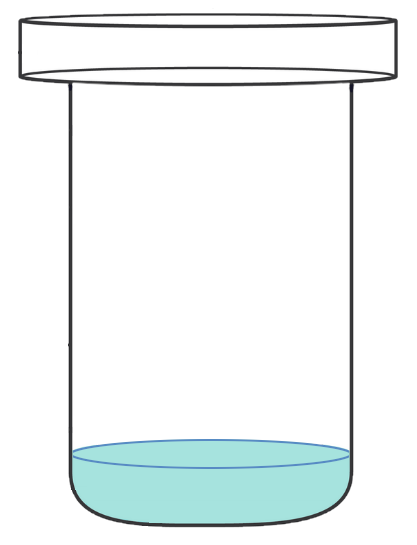
\includegraphics[height=0.15\textheight]{images/CCM/CCM_etapes_cuve.png}
    \end{center}
    
    \vspace*{-12pt}
    Remplir jusqu'à environ 0,5 cm de hauteur d'éluant la cuve à CCM.
  }{
    \begin{center}
      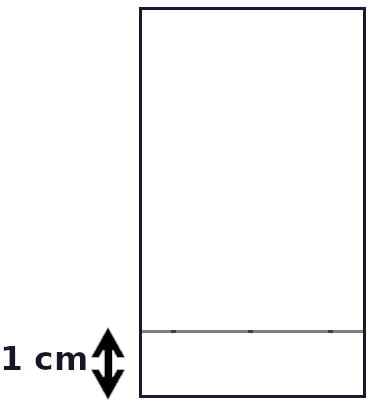
\includegraphics[height=0.15\textheight]{images/CCM/CCM_etapes_trait.png}
    \end{center}
    
    \vspace*{-12pt}
    À environ 1 cm du bord inférieur, tracer au crayon à papier un trait fin.
    Vérifier que le trait est au-dessus du niveau de l'éluant.
  }{
    \begin{center}
      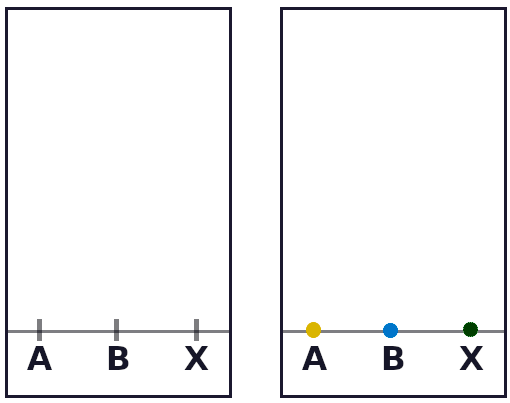
\includegraphics[height=0.15\textheight]{images/CCM/CCM_etapes_depot.png}
    \end{center}
    
    \vspace*{-12pt}
    Marquer les emplacements des échantillons à déposer.
    Prélever chaque échantillon avec un cure dent et les déposer sur l'emplacement prévu.
  }
  
  \bigskip
  
  \separationDeuxBlocs{
    \begin{center}
      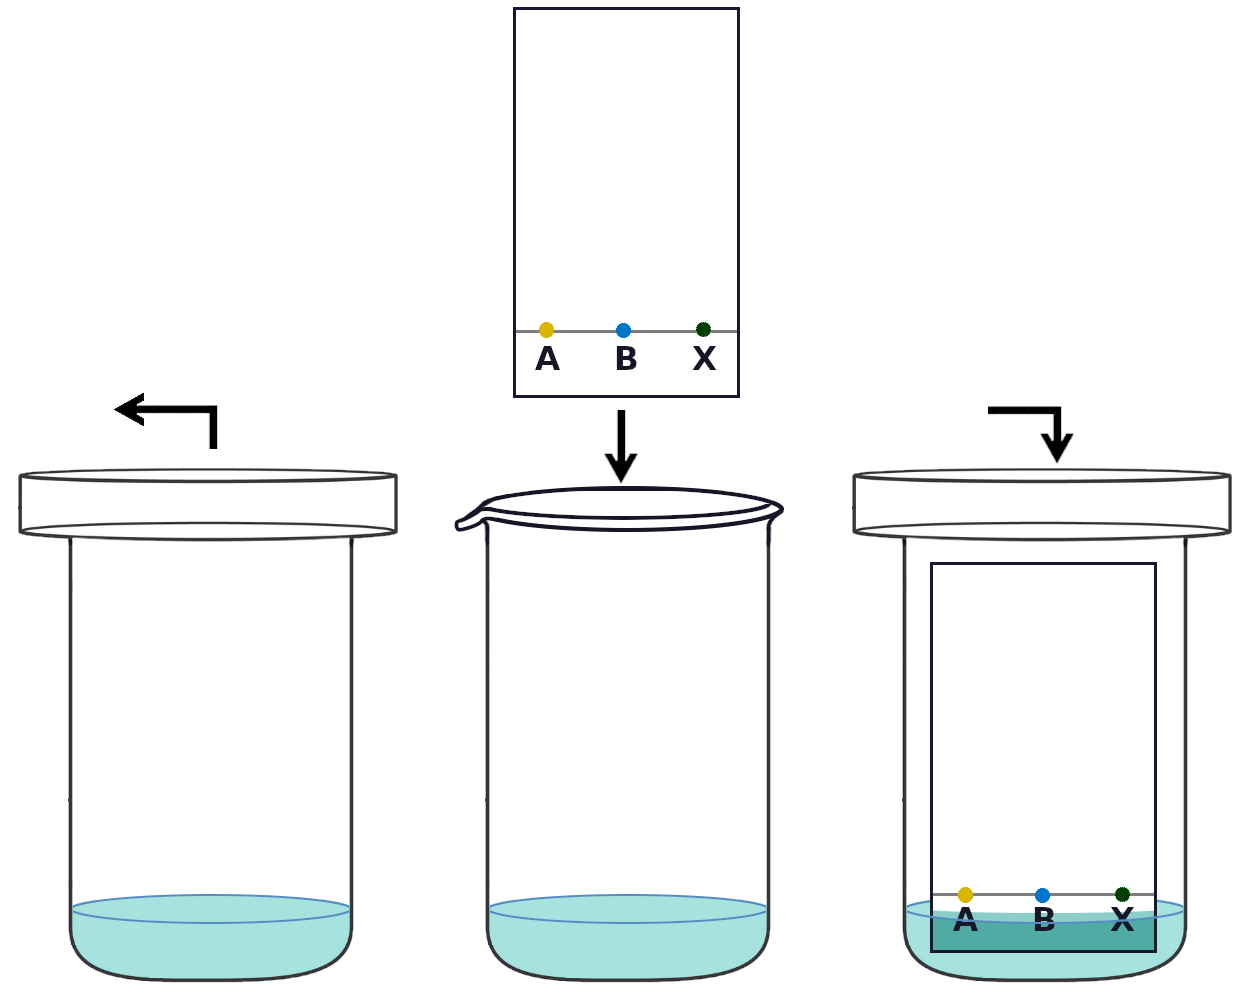
\includegraphics[height=0.25\textheight]{images/CCM/CCM_etapes_ajout.png}
    \end{center}
    
    \vspace*{-12pt}
    Introduire délicatement la plaque dans la cuve en la tenant par les côtés.
    Refermer la cuve.
    \textbf{Ne jamais déplacer la cuve} et attendre que l'éluant monte.
  }{
    \begin{center}
      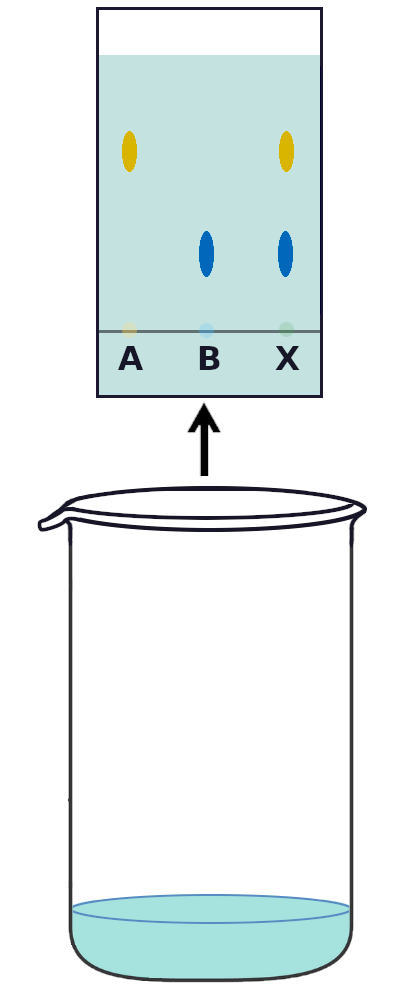
\includegraphics[height=0.25\textheight]{images/CCM/CCM_etapes_retrait.png}
    \end{center}
    
    \vspace*{-12pt}
    Quand le front de l'éluant s'approche du bord supérieur, sortir la plaque.
    Tracer immédiatement une ligne indiquant la hauteur où l'éluant est monté.
  }
\end{doc}


%%%% questions
\exo{
  Placer quelques gouttes de sirop vert dans un bécher de $50\unit{mL}$. Ajouter environ $10\unit{mL}$ d'eau distillée et agiter.\competence{REA}
}{0}

\exo{
  Réaliser le protocole du document 3, avec un dépôt de colorant jaune, un dépôt de colorant bleu et  et un dépôt de la solution préparée à la question 1.\competence{REA}
}{0}

\exo{
  Coller ici le chromatogramme \textbf{sec} et entourer les différentes tâches au crayon à papier.\competence{REA}
}{0}
\vspace*{240pt}

\newpage
\exo{
  Pourquoi doit-on placer la ligne de dépôt au dessus du niveau de l'éluant ?\competence{ANA/RAI}
}{2}

\exo{
  Pourquoi ne doit-on pas déplacer la cuve pendant la montée de l'éluant ?\competence{ANA/RAI}
}{2}

\exo{
  En analysant le chromatogramme à l'aide du document 2, indiquer si les échantillons sont des corps purs ou des mélanges.\competence{APP}
}{3}

\exo{
  En utilisant le chromatogramme, que contient le colorant vert du sirop ? Justifier avec des arguments simples.\competence{APP, VAL}
}{2}


% \newpage
% \exo{Relier chaque verrerie à son nom.}{0}

% %%
% \newcommand{\centeredBullet}{\centering\textbullet}
% \vspace*{-12pt}
% \begin{center}
%   \image{1}{images/instruments_chimie/instruments_1.png}
  
%   \begin{tabular}{
%     m{0.23\textwidth} m{0.23\textwidth} m{0.23\textwidth} m{0.23\textwidth} m{12pt}
%   }
%     \centeredBullet & \centeredBullet & \centeredBullet & \centeredBullet & \phantom{b}
%     \\[48pt]
%     \centeredBullet & \centeredBullet & \centeredBullet & \centeredBullet & \phantom{b}
%     \\
%     \centering sabot de pesée  &  \centering tube à essai  &  \centering coupelle de pesée  & \centering verre à pied &
%   \end{tabular}
% \end{center}

% %%
% \vspace{12pt}
% \begin{center}
%   \image{1}{images/instruments_chimie/instruments_2.png}
  
%   \begin{tabular}{
%     m{0.21\textwidth} m{0.23\textwidth} m{0.25\textwidth} m{0.28\textwidth} m{12pt}
%   }
%     \centeredBullet & \centering\textbullet & \centeredBullet & \centeredBullet & \phantom{b}
%     \\[48pt]
%     \centeredBullet & \centeredBullet & \centeredBullet & \centeredBullet & \phantom{b}
%     \\
%     \centering éprouvette graduée  &  \centering bécher &  \centering fiole jaugée  & \centering erlenmeyer &
%   \end{tabular}
% \end{center}
  % %%%% début de la page
\newpage
\enTete{Corps purs et solutions}{1}


%%%% titre
\vspace*{-36pt}
\numeroActivite{4}
\titreTP{Dosage d'un antiseptique}
%\nomPrenomClasse


%%%% objectifs
\begin{objectifs}
  \item Apprendre le vocabulaire sur les solutions.
  \item Comprendre la notion de concentration massique.
  \item Doser la quantité de permanganate de potassium présente dans du Dakin.
\end{objectifs}


%%%% contexte
\begin{encart}
  \emphase{Contexte :}
  
  Le Dakin est une solution antiseptique qui sert à nettoyer des plaies. Le principe actif du Dakin est stabilisé par l'ajout de permanganate de potassium \chemfig{K MnO_4}.
  Le permanganate de potassium donne une teinte violette au Dakin.
\end{encart}

\problematique{Comment mesurer la concentration en permanganate de potassium présente dans le Dakin ?}


%%%% documents
\begin{doc}{Solution, solvant et soluté}
  \label{doc:solution}
  \vspace*{-24pt}
  \begin{encart}
    \chevron Une \important{solution} est un mélange homogène. \\
    Le \important{solvant} est le composant majoritaire du mélange. Le \important{soluté} est l'espèce qui est dispersée dans le solvant.
  \end{encart}
  
  \begin{center}
    \important{Solvant + Soluté(s) = Solution}
  \end{center}
  
  \begin{encart}
    On parle de \important{solution aqueuse} si le solvant est l'eau \chemfig{H_2 O}.
  \end{encart}
\end{doc}


%%%%
\begin{doc}{Concentration en soluté}
  \label{doc:concentration}
  \vspace*{-24pt}
  \begin{encart}
    La \important{concentration massique $\mathbf{c}$} mesure la quantité de soluté présent dans une solution.
    C'est le rapport de la masse $m$ de \textbf{soluté} dissous dans le volume $V$ de la \textbf{solution}
    \begin{equation}
      c = \frac{m_\text{soluté}}{V_\text{solution}}
    \end{equation}
  \end{encart}
  
  \attention Il faut bien distinguer \textbf{concentration massique} et \textbf{masse volumique}.
  La concentration mesure la masse de soluté contenue dans une solution.
  La masse volumique mesure la masse d'un échantillon contenue dans un volume donné.
\end{doc}


%%%%
\newpage
\begin{doc}{Dakin}
  \label{doc:dakin}
  Le Dakin est une solution aqueuse d'hypochlorite de sodium \chemfig{Na ClO}.
  Du permanganate de potassium \chemfig{K MnO_4} est ajouté à la solution, pour qu'elle ne soit pas dégradée par l'exposition au rayonnement UV du Soleil.
  
  \fleche Le constructeur indique que la concentration de \chemfig{KMnO_4} est de l'ordre de $0,\!01 \unit{g/L}$ dans le Dakin.
\end{doc}


%%%%
\begin{doc}{Mesure de concentration}
  \label{doc:dosage}
  \vspace*{-24pt}
  \begin{encart}
    On parle de \important{dosage} quand on mesure la concentration d'une espèce chimique présente dans une solution.
    
    Un \important{dosage par étalonnage} consiste à déterminer la concentration d’une espèce chimique en comparant une grandeur physique caractéristique de la solution, à la même grandeur physique mesurée pour des solutions étalon.
  \end{encart}
  
  \begin{encart}
    Une \important{échelle de teinte} permet de mesurer la concentration d'un soluté coloré.
    \vspace*{-16pt}
  \end{encart}

  La teinte d'une solution est proportionnelle à la concentration en soluté.
  En préparant une série de solutions de concentrations connues, une \textbf{gamme}, et en comparant les teintes, on va pouvoir encadrer la valeur de la concentration de la solution que l'on veut mesurer.
  
  \bigskip
  
  \attention Il faut comparer les teintes avec des verreries identiques, la teinte s'assombrit avec l'épaisseur.
  
  \attention La solution dont on veut mesurer la concentration doit avoir une teinte comprises dans la gamme réalisée !
\end{doc}
 

%%%%
\begin{doc}{Dilution d'une solution}
  \label{doc:dilution}
  \vspace*{-24pt}
  \begin{encart}
    La \important{dilution} est la diminution de la concentration d'une solution par ajout de solvant, sans ajout de soluté.
    La solution est diluée.
  \end{encart}
  On parle de \textbf{solution mère} pour la solution de départ et de \textbf{solution fille} pour la solution obtenue.
  
  Le facteur de dilution est le rapport des concentrations des solutions mère et fille.
  Ce rapport est égal au volume de la solution fille sur le volume de la solution mère
  \begin{equation*}
    F = \frac{c_\text{mère}}{c_\text{fille}}
      = \frac{V_\text{fille}}{V_\text{mère}}
  \end{equation*}
\end{doc}


%%%%
\begin{doc}{Protocole d'une dilution}
  \label{doc:protocole_dilution}
  \begin{center}
    \image{1}{images/protocoles/protocole_dilution.png}
  \end{center}
  
  \vspace*{-24pt}
  
  \begin{enumerate}
    \item Prélever le volume $V_\text{mère}$ de la solution mère à l'aide de la pipette graduée.
    Le bas du ménisque doit atteindre la graduation supérieure.
    \item Introduire la solution prélevée dans la fiole jaugée de volume $V_\text{fille}$.
    \item Ajouter de l'eau distillée dans la fiole jaugée jusqu'aux $2/3$ et agiter doucement. Compléter jusqu'à ce que le bas du ménisque atteigne le trait de jauge.
    \item Fermer la fiole et l'agiter en la retournant plusieurs fois.
    \item Verser la solution fille obtenue dans un bécher.
  \end{enumerate}
\end{doc}


%%% Questions
\vspace*{12pt}
\exo{
  \docu{\ref{doc:solution}, \ref{doc:dakin}} Donner le solvant et les solutés de la solution de Dakin.
}{4}


%
\vspace*{-3pt}
\exo{
  \docu{\ref{doc:concentration}} On dispose d'une solution mère de volume $V_\text{mère} = 20 \unit{mL}$, avec une concentration de permanganate de potassium $c_\text{mère} = 0,\!04 \unit{g/L}$.
  Calculer la masse de permanganate de potassium dans la solution.
}{2}


%
\exo{
  \docu{\ref{doc:dosage}, \ref{doc:dilution}} On souhaite réaliser une échelle de teinte composée de 4 solutions étalon pour mesurer la concentration de permanganate de potassium dans le Dakin.

  \begin{center}
    \setlength{\extrarowheight}{4pt}
    \begin{tabular}{c | c | c | c | c}
      Solution étalon & \phantom{00}1\phantom{00} & \phantom{00}2\phantom{00}& \phantom{00}3\phantom{00} & \phantom{00}4\phantom{00} \\
      \hline
      Concentration (g/L) &  &  &  & 
    \end{tabular}
  \end{center}
  
  Donner le facteur de dilution entre les différentes solutions.
}{1}


%
\exo{
  \docu{\ref{doc:dakin}} Justifier l’intervalle des concentrations proposées pour l’échelle de teinte, à partir de la valeur attendue de la concentration en permanganate de potassium.
}{1}


%
\exo{
  \docu{\ref{doc:dilution}, \ref{doc:protocole_dilution}}
  Sachant que le volume de la fiole jaugée est de $50\unit{mL}$, donner le volume de la solution mère à prélever pour avoir un facteur de dilution $F = 2$.
}{2}


%
\exo{
  \docu{\ref{doc:protocole_dilution}} Réaliser l'échelle de teinte en effectuant trois dilutions successives.
  Verser quelques millilitres de chaque solutions dans des tubes à essais.
}{0}


%
\vspace*{8pt}
\exo{
  \docu{\ref{doc:dakin}, \ref{doc:dosage}} Utiliser l'échelle de teinte pour encadrer la valeur de la concentration en permanganate de potassium dans le Dakin.
  Est-elle cohérente avec celle du constructeur ?
}{2}


%
\exo{
  Proposer une autre échelle de teinte pour améliorer la précision de la mesure (donner une liste de concentration).
}{1}
  % %%%% début de la page
\newpage
\enTete{Corps purs et solutions}{1}

%%%%
\nomPrenomClasse

%%%% titre
\numeroActivite{5}
\titreTP{Dosage d'un antiseptique -- Identification d'espèces chimiques}


%%%% objectifs
\begin{objectifs}
  \item Réaliser une échelle de teinte \textbf{en autonomie.}
  \item Mesurer la concentration en \chemfig{KMnO_4} présente dans du Dakin.
  \item Réaliser des tests chimiques.
\end{objectifs}


%%%%
\titrePartie{Dosage d'un antiseptique}


%%%% evaluation
\begin{tableauCompetences}
  \centering APP --
  Rechercher l'information.
  & & & &
  \\ \hline
  %
  \centering ANA/RAI --
  Élaborer un protocole.
  & & & &
  \\ \hline
  %
  %
  \centering REA --
  Réaliser un protocole, un calcul.
  & & & &
  \\ \hline
  %
  \centering VAL --
  Comparer avec des valeurs de références.
  & & & &
\end{tableauCompetences}


\bigskip
\problematique{Mesurer la concentration de permanganate de potassium présent dans du Dakin à l'aide d'une échelle de teinte.}


%%%%
\begin{doc}{Dakin}
  \label{doc:dakin}
  Le Dakin est une \textbf{solution aqueuse} d'hypochlorite de sodium (\chemfig{Na ClO}).
  Du permanganate de potassium (\chemfig{K MnO_4}) est ajouté à la solution, pour qu'elle ne soit pas dégradée par l'exposition au rayonnement UV du Soleil.
  
  \fleche Le constructeur indique que la concentration de \chemfig{KMnO_4} est de l'ordre de $0,\!01 \unit{g/L}$ dans le Dakin.
  
  \fleche On dispose d'une solution de permanganate de potassium (\chemfig{K MnO_4}) avec une concentration massique $c = 0,\!08 \unit{g/L}$.
\end{doc}


%%%%
\question{
  Donner une série de concentration pour des solutions étalons, de sortes que l'échelle de teinte réalisée permette d'encadrer la concentration annoncée par le constructeur.\competence{APP, ANA/RAI}
}{0}

\begin{center}
  \setlength{\extrarowheight}{4pt}
  \begin{tabular}{c | c | c | c | c}
    Solution étalon & \phantom{00}1\phantom{00} & \phantom{00}2\phantom{00}& \phantom{00}3\phantom{00} & \phantom{00}4\phantom{00} \\
    \hline
    Concentration (g/L) & 0,08 &  &  & 
  \end{tabular}
\end{center}


%%%%
\question{
  Indiquer les volumes des solutions mère $V_\text{mère}$ à introduire dans une fiole jaugée de $50 \unit{mL}$ pour préparer chaque solution.\competence{REA}
}{0}
  
\begin{center}
  \setlength{\extrarowheight}{4pt}
  \begin{tabular}{c | c | c | c}
    Solution étalon & \phantom{00}2\phantom{00}& \phantom{00}3\phantom{00} & \phantom{00}4\phantom{00} \\
    \hline
    $V_\text{mère}$ (mL) &  &  &
  \end{tabular}
\end{center}

\appelProf Appeler le professeur si vous êtes bloqué-es.


%%%%
\question{
  Préparer les solutions étalons par dilution successives.\competence{REA}
}{0}


%%%%
\question{
  En utilisant l'échelle de teinte réalisée, donner un encadrement pour la concentration de permanganate de potassium présent dans le Dakin.
  La réponse doit être rédigée.\competence{REA, VAL}
}{3}

\appelProf Appeler le professeur si vous êtes bloqué-es.


%%%%
\question{
  Indiquer si votre mesure est cohérente avec la concentration annoncée par le constructeur.\competence{APP, VAL}
}{2}


%%%%
\newpage
\vspace*{-36pt}
\titrePartie{Identification d'espèces chimiques}

%%%% contexte
\begin{encart}
  \emphase{Contexte :}
  
  Les eaux minérales sont des solutions aqueuses, qui contiennent plusieurs ions de nature et de masses différentes.
  Impropre à une consommation régulière, elles peuvent servir dans des régimes spécifiques.
\end{encart}

\problematique{Comment déterminer les ions présents dans des eaux minérales ?}


%%%% documents
\begin{doc}{Composition de trois eaux minérales}
  \label{doc:composition_eau}
  \vspace*{-24pt}
  \begin{center}
    \textbf{Vichy St Yorre}
    
    \setlength{\extrarowheight}{6pt}
    \begin{tabular}{l r|l r}
      \rowcolor{gray!20} \multicolumn{4}{c}{Minéralisation en mg/L}
      \\ \hline
      Bicarbonates (\chemfig{CO_3^{2-}}) & 4368 &
      Chlorures    (\chemfig{Cl^{-}})    & 322  \\ \hline
      Sodium       (\chemfig{Na^+})      & 1708 &
      Sulfates     (\chemfig{SO_4^{2-}}) & 174  \\ \hline
      Potassium    (\chemfig{K^+})       & 110  &
      Calcium      (\chemfig{Ca^{2+}})   & 90   \\ \hline
      Fluorures    (\chemfig{F^{-}})     & 1    &
      Magnésium    (\chemfig{Mg^{2+}})   & 11   \\ \hline
    \end{tabular}

    %
    \vspace*{12pt}
    \textbf{Volvic}
    
    \setlength{\extrarowheight}{6pt}
    \begin{tabular}{l r|l r}
      \rowcolor{gray!20} \multicolumn{4}{c}{Minéralisation en mg/L}
      \\ \hline
      Bicarbonates (\chemfig{CO_3^{2-}}) & \phantom{1}65,3 &
      Chlorures    (\chemfig{Cl^{-}})    & 8,4  \\ \hline
      Sodium       (\chemfig{Na^+})      & \phantom{1}9,4  &
      Sulfates     (\chemfig{SO_4^{2-}}) & 6,9  \\ \hline
      Potassium    (\chemfig{K^+})       & 5,7  &
      Calcium      (\chemfig{Ca^{2+}})   & 9,9  \\ \hline
      Nitrates     (\chemfig{NO_3^{-}})  & 6,3  &
      Magnésium    (\chemfig{Mg^{2+}})   & 6,1  \\ \hline
    \end{tabular}

    %
    \vspace*{12pt}
    \textbf{Hépar}
    
    \setlength{\extrarowheight}{6pt}
    \begin{tabular}{l r|l r}
      \rowcolor{gray!20}
      \multicolumn{4}{c}{Minéralisation en mg/L}
      \\ \hline
      Bicarbonates (\chemfig{CO_3^{2-}}) & 383,7 &
      Chlorures    (\chemfig{Cl^{-}})    & 11    \\ \hline
      Sodium       (\chemfig{Na^+})      & 14,2  &
      Sulfates     (\chemfig{SO_4^{2-}}) & 1479  \\ \hline
      Potassium    (\chemfig{K^+})       & 4     &
      Calcium      (\chemfig{Ca^{2+}})   & 549   \\ \hline
      Nitrates     (\chemfig{NO_3^{-}})  & 4,3   &
      Magnésium    (\chemfig{Mg^{2+}})   & 119   \\ \hline
    \end{tabular}
  \end{center}
\end{doc}


%%%%
\newpage
\begin{doc}{Tests caractéristiques de certains ions}
  \label{doc:tests_ions}
  \vspace*{-12pt}
  \begin{center}
    \setlength{\extrarowheight}{6pt}
    \begin{tabular}{| c | c | c |}
      \hline
      \rowcolor{gray!20}
      Ion à tester & Réactif utilisé & Résultat du test positif 
      \\ \hline
      %
      Chlorures (\chemfig{Cl^{-}}) &
      Solution de nitrate d'argent &
      Précipité blanc, noircit* \\ \hline
      %
      Sulfates  (\chemfig{SO_4^{2-}}) &
      Solution de chlorure de baryum &
      Précipité blanc \\ \hline
      %
      Calcium (\chemfig{Ca^{2+}}) &
      Solution d'oxalate d'ammonium &
      Précipité blanc \\ \hline
      %
      Magnésium (\chemfig{Mg^{2+}}) &
      Solution d'hydroxyde de sodium &
      Précipité blanc \\ \hline
    \end{tabular}
    
    \bigskip
    * Le précipité blanc noircit à la lumière.
  \end{center}
\end{doc}


%%%%
On a trois béchers (A, B, C) contenant des eaux minérales, que vous voulez identifier.

\question{
  Réaliser le protocole suivant :
  \begin{enumerate}
    \item Laver et sécher 4 tubes à essais.
    \item Verser dans chaque tube à essais quelques mL de l'eau d'un bécher.
    \item Réaliser un test différent dans chaque tube à essais à l'aide des 4 réactifs.
    \item Noter si un précipité se forme et son abondance dans le tableau suivant ($-$, $+$, $++$, $+++$)
  \end{enumerate}
}{0}

\begin{center}
  \setlength{\extrarowheight}{10pt}
  \begin{tabular}{l | c | c | c}
    \rowcolor{gray!20} Test réalisé & Bécher A & Bécher B & Bécher C \\ \hline
    Nitrate d'argent    & & & \\ \hline
    Chlorure de baryum  & & & \\ \hline
    Oxalate d'ammonium  & & & \\ \hline
    Hydroxyde de sodium & & &
  \end{tabular}
\end{center}

\question{
  En vous aidant des documents~\ref{doc:composition_eau} et~\ref{doc:tests_ions}, en déduire l'eau minérale contenu par chaque bécher.
}{3}
  
  %% Chapitre 2
  % %%%% début de la page
\sndEnTeteDeux

%%%%
\nomPrenomClasse


%%%% titre
\numeroActivite{1}
\titreActivite{Décrire le mouvement}


%%%% objectifs
\begin{objectifs}
  \item Décrire un mouvement.
  \item Comprendre la notion de référentiel.
  \item Comprendre que le mouvement dépend du référentiel.
\end{objectifs}


%%%% evaluation
\begin{tableauCompetences}
  \centering APP &
  Rechercher l'information.
  
  Représenter la situation par un schéma.
  & & & &
  \\ \hline
  \centering ANA/RAI &
  Proposer une stratégie de résolution.
  & & & &
\end{tableauCompetences}

%%%%
\vspace*{6pt}
\begin{doc}{Un peu de vocabulaire}
  \vspace*{-24pt}
  \begin{encart}
    \important{Système} : objet dont on étudie le mouvement.
  \end{encart}
  
  \begin{encart}
    \important{Trajectoire} : ensemble des positions successives occupées par le système.
  \end{encart}
  
  Le \important{mouvement} d'un système est donné par la description de sa trajectoire + l'évolution de sa vitesse.
\end{doc} 


\vspace*{2pt}
\begin{doc}{Type de trajectoires}
  \label{doc:trajectoires}

  Trajectoire \important{rectiligne} : trajectoire représentée par \dotfill \\[4pt]
  Trajectoire \dotfill : trajectoire représentée par un cercle. \\[4pt]
  Trajectoire \important{curviligne} : trajectoire représentée par \dotfill
\end{doc}


\vspace*{2pt}
\begin{doc}{Vitesse et accéleration}
  \label{doc:vitesse}

  Vitesse \important{uniforme} (constante) : le système n’accélère pas. \\[4pt]
  La vitesse augmente : le système \dotfill \\[4pt]
  La vitesse diminue : le système \dotfill \\[4pt]
  Si la vitesse est \dotfill on dit que le système est \important{immobile}.
\end{doc}


%%%%
\newpage

\question{Compléter les documents~\ref{doc:trajectoires} et~\ref{doc:vitesse}.}{0}

\fleche Pour la suite de cette activité, vous allez choisir entre l'étude du mouvement des oies ou de la Lune.
Vous présenterez ensuite les résultats de votre étude au reste de la classe à l'oral.


%%%%
\titreSection{\'Etude du mouvement des oies}

Le compteur du bateau affiche une vitesse $v_\text{bateau} = 3,\!6 \times 10^1 \unit{km/h}$.

\vspace*{6pt}
\question{Pour la personne qui filme les oies, quelle est la vitesse des oies ?}{0}
\question{Pour une personne se trouvant sur la berge, quelle est la vitesse des oies ?}{0}
\question{Schématiser la trajectoire des oies si on les observe depuis la berge.}{0}
\question{Indiquer le mouvement des oies depuis le bateau et la berge.}{0}

\titreSection{\'Etude du mouvement de la Lune}

La Lune tourne autour de la Terre à une vitesse $v_\text{Lune} = 3,\!7 \times 10^3 \unit{km/h}$ et la Terre tourne autour du Soleil à une vitesse $v_\text{Terre} = 1,\!1 \times 10^5 \unit{km/h}$.

\begin{figure}[!ht]
  \begin{subfigure}{0.48\linewidth}
    \centering
    \image{0.8}{images/mouvements/terre_lune.png}
    \caption{Point de vue centré sur la Terre}
    \label{fig:terre_lune}
  \end{subfigure}
  \begin{subfigure}{0.48\linewidth}
    \centering
    \image{0.8}{images/mouvements/terre_lune_soleil.png}
    \caption{Point de vue centré sur le Soleil}
    \label{fig:terre_lune_soleil}
  \end{subfigure}
\end{figure}

\vspace*{-6pt}
\question{Depuis le point de vue centré sur la Terre, quelle est la vitesse de la Lune ?}{0}
\question{Schématiser la trajectoire de la Lune depuis ce point de vue et indiquer son mouvement.}{0}
\question{Peut-on décrire la vitesse de la Lune depuis le point de vue centré sur le Soleil ?}{0}
\question{Schématiser la trajectoire de la Lune depuis ce point de vue.}{0}


\titreSection{Notion de référentiel}

\question{Convertir la vitesse $v_\text{Lune}$ en m/s.
\textit{Rappel : } $1\unit{km} = 10^3\unit{m}$, $1\unit{h} = 3,\!6 \times 10^3 \unit{s}$.}{0}
\question{Quelle distance la Lune parcours pendant 1 seconde ? Comparer avec la longueur de sa trajectoire, qui est de $2,4\times 10^6 \unit{km}$}{0}
\question{Est-ce que la seconde est une durée d'observation suffisante pour décrire la trajectoire de la Lune ?}{0}
\question{Conclusion : pourquoi est-il important de définir le référentiel, qui est l’endroit où on se place et le temps passé à observer, avant d'étudier un mouvement ?}{0}

\feuilleBlanche
  % %%%% début de la page
\sndEnTeteDeux

%%
\nomPrenomClasse


%%%% titre
\numeroActivite{2}
\titreActivite{Chute d'une balle}


%%%% objectifs
\begin{objectifs}
  \item Comprendre la notion de vecteur vitesse.
  \item Tracer des vecteurs vitesses.
\end{objectifs}


%%%% evaluation
\begin{tableauCompetences}
  \centering S'Approprier (APP) &
  Représenter la situation par un schéma.
  & & & &
  \\ \hline
  \centering Communication (COM) &
  Travailler en groupe, échanger entre élèves.
  & & & &
\end{tableauCompetences}


%%
\vspace*{6pt}
\problematique{Quelle est l'influence d'une translation sur la description du mouvement d'un objet ?}


%%%% documents
\begin{doc}{Chronophotographie de la chute d'une balle}
  \label{doc:chrono}
  \vspace*{-20pt}
  \begin{center}
    \image{0.9}{images/mouvements/chronophotographie_balle.png}
  \end{center}
  Une chronophotographie est une superposition de plusieurs images prises les unes après les autres avec un intervalle de temps régulier.
  Pour réaliser cette chronophotographie, \textbf{on a pris une image toutes les} $\mathbf{40} \unit{\mathbf{ms}}$.
  \bigskip
  
  Réaliser une chronophotographie permet de repérer des positions par lesquelles passent la balle, ce qui est impossible à l'oeil nu.
  Les ronds indiquent les positions de la balle, les carrés indiquent les positions du centre de masse de l'homme sur la trottinette.
\end{doc}

%%
\begin{doc}{Vecteur}
  \label{doc:vecteur}
  \vspace*{-24pt}
  \begin{encart}
    \important{Vecteur} : objet mathématique représenté par un segment fléché $\longrightarrow$ et noté avec une lettre surmontée d'une flèche $\vv{v}$.
    
    Un vecteur contient quatre information : une \important{direction}, un \important{sens}, une \important{norme,} et un \important{point d'application} (ou origine).
  
    Un vecteur est \important{constant} si sa direction, son sens et sa norme ne varie pas le long du mouvement.
  \end{encart}
\end{doc}

%%
\begin{doc}{Vecteur déplacement et vecteur vitesse d'un point}
  \label{doc:vitesse}
  Soient $P_1$ la position d'un point à l'instant $t_1$ et $P_3$ la position de ce même point à l'instant $t_3$.
  Le déplacement du point matériel entre les dates $t_1$ et $t_3$ est défini par le vecteur déplacement $\vv{P_1 P_3}$.
  Graphiquement, c'est la flèche qui relie $P_1$ à $P_3$. 
  \bigskip
  
  Le vecteur $\vv{P_1 P_3}$ est caractérisé par
  \begin{listePoints}
    \item une direction : celle de la droite $P_1 P_3$.
    \item Un sens : de $P_1$ vers $P_2$.
    \item Une norme : égale à la distance $P_1 P_3$ en mètre (m).
    \item Une origine : le point $P_1$
  \end{listePoints}
  
  \begin{encart}
    Le \important{vecteur vitesse} $\vv{v_2}$ d'un système au point $P_2$ entre les instants $t_1$ et $t_3$ a pour expression
    \begin{equation}
      \vv{v_2} = \frac{\vv{P_1 P_3}}{t_3 - t_1}
    \end{equation}
  \end{encart}
  
  Le vecteur $\vv{v_2}$ est caractérisé par :
  \begin{listePoints}
    \item une direction : parallèle au segment $P_1 P_3$ et tangent à la trajectoire.
    \item Un sens : le sens du mouvement.
    \item Une norme : $v_2 
    = \norm{\vv{v_2}}
    = \displaystyle \norm{\frac{\vv{P_1 P_3}}{t_3 - t_1}}
    = \displaystyle \frac{P_1 P_3}{t_3 - t_1}$.
    \item Une origine : $P_2$.
  \end{listePoints}
  $P_1 P_3$ est la distance entre les points $P_1$ et $P_3$ en mètre (m). $t_3 - t_1$ est la durée séparant les instants $t_1$ et $t_3$ en seconde (s). $v_2$ est la norme de la vitesse en mètre par seconde (m/s).
\end{doc}



%%%%
\newpage
\titreSection{Mouvement dans le référentiel de \lignePointillee{0.2}}

%
\exo{
  Quel est le référentiel utilisé pour décrire le mouvement de la balle et de l'homme sur la trottinette ici ?
}{1}


%%
\titreSousSection{Mouvement de l'homme sur la trottinette}

%
\exo{
  Quelle est la trajectoire de l'homme sur la trottinette ?
}{1}

%
\exo{
  Comment évolue la vitesse de l'homme sur la trottinette ? Indiquer la nature de son mouvement.
}{2}


%%%%
\titreSousSection{Mouvement de la balle}

%
\exo{
  Repérer sur la chronophotographie du document~\ref{doc:chrono}, le point de départ de la balle.
  On notera $P_1$ cette position.
  Numéroter les positions successives de la balle, que l'on notera $P_2, P_3, \ldots P_8$
}{0}

%
\exo{
  Tracer sur la photo du document~\ref{doc:chrono} le vecteur $\vv{P_2 P_3}$ et le vecteur $\vv{P_5 P_7}$.
}{0}

%
\exo{
  En utilisant l'échelle sur la photo, déterminer les normes en mètre de ces deux vecteurs.
  Indiquer si ces normes sont identiques.
}{2}

%
\exo{
  Calculer la norme en mètre par seconde de ces deux vecteurs, en vous aidant du document~\ref{doc:vitesse}.
}{2}

%
\exo{
  Schématiser le vecteur vitesse $\vv{v_2}$ entre les points $P_2$ et $P_3$ et le vecteur vitesse $\vv{v_6}$ entre les points $P_5$ et $P_7$, en vous aidant du document~\ref{doc:vitesse}.
}{0}

\feuilleBlanche

%%%%
% \newpage
% \titreSection{Mouvement dans le référentiel de la trottinette}
% 
% %
% \exo{
%   Ouvrir la vidéo de la de chute balle dans le logiciel Tracker.
% }{0}
% 
% %
% \exo{
%   Repérer dans la vidéo le moment où la balle commence à tomber. 
% }{0}
% 
% %
% \exo{
%   Sur la vidéo, réaliser le pointage de la balle.
% }{0}
% 
% %
% \exo{
%   Tracer la norme de la vitesse, la vitesse selon l'axe $x$ et la vitesse selon l'axe $y$.
%   Que remarquez vous pour la vitesse selon l'axe $x$ ?
% }{2}
% 
% %
% \exo{
%   Que pouvez-vous en déduire sur la nature du mouvement de la balle dans le référentiel de la trottinette ?
%   Représenter avec un schéma sa trajectoire.
% }{2}
% \vspace{200pt}
% 
% %
% \exo{
%   Conclure sur la position de la balle au moment où elle touche le sol par rapport à la trottinette.
% }{2}
  % %%%% début de la page
\sndEnTeteDeux

%%
\nomPrenomClasse


%%%% titre
\numeroActivite{3}
\titreActivite{Modéliser le mouvement}


%%%% objectifs
\vspace{-10pt}
\begin{objectifs}
  \item Comprendre les limites du modèle du point matériel.
  \item Comprendre la notion de référentiel.
  \item Comprendre la notion de vecteur.
\end{objectifs}


%%%% evaluation
\begin{tableauCompetences}
  \centering Communication (COM) &
  Travailler en groupe, échanger entre élèves.
  & & & &
\end{tableauCompetences}


%%%%
\titreSection{Système et référentiel}

%%%%
\vspace{-10pt}
\begin{doc}{Modèle du point matériel}
  \vspace*{-24pt}
  \begin{encart}
    \important{Système} : objet dont on étudie le mouvement.
  
    On ne va s'intéresser qu'au mouvement global du système.
    C'est pourquoi on va modéliser le système par \dotfill \\[8pt]
    \reponse{1}
    \vspace*{-12pt}
    %un point de même masse, localisé en son centre de masse.
    %C'est le \important{modèle du point matériel}.
  \end{encart}

  \fleche Le modèle du point matériel revient à oublier toute information sur la géométrie du système étudié. 
  Les éventuelles rotations et déformations ne sont donc pas prises en compte.
\end{doc}


\begin{tabularx}{\linewidth}{ m{0.2\linewidth} | m{0.2\linewidth} | m{0.25\linewidth} | m{0.26\linewidth} }
  \rowcolor{gray!20}
  \centering Système & Centre de masse & \centering Trajectoire & Informations perdues
  \\ \hline
  %
  \centering
  \phantom{\small b} \newline
  \image{0.8}{images/mouvements/point_balle_tennis.png}
  \newline
  Balle de tennis &
  \centering Centre de la balle & &
  \\ \hline
  %
  \centering
  \phantom{\small b} \newline
  \image{0.8}{images/mouvements/point_roue.jpg} \newline
  Roue &
  \centering Centre de la roue & &
  \\ \hline
\end{tabularx}
\newpage

\vspace*{-30pt}
\begin{tabularx}{\linewidth}{ m{0.2\linewidth} | m{0.2\linewidth} | m{0.25\linewidth} | m{0.3\linewidth} }
  \hline
  %
  \centering
  \phantom{\small b} \newline
  \image{0.8}{images/mouvements/point_humain_course.jpg}
  \newline
  Modèle d'humain &
  \centering Nombril & &
  \\ \hline
\end{tabularx}

%%
\begin{doc}{Référentiel}
  Pour décrire le mouvement, il faut pouvoir le repérer dans l’espace et dans le temps, pour ça on utilise un référentiel.
  
  \begin{encart}
    \important{Référentiel} : objet de référence, muni d'un \dotfill, \newline
    par rapport auquel on étudie le mouvement du système.
  \end{encart}
  
  \begin{encart}
    La description du mouvement dépend du \important{référentiel} choisi. On appelle ça la \important{relativité} du mouvement.
  \end{encart}
\end{doc}


%%%%
\titreSection{Vecteur}

%%
\begin{doc}{Vecteur en physique}
  \label{doc:vecteur}
  \vspace*{-24pt}
  \begin{encart}
    \important{Vecteur} : objet mathématique représenté par un segment fléché $\longrightarrow$ et noté avec une lettre surmontée d'une flèche $\vv{v}$.
    
    Un vecteur contient quatre information : 
    \begin{listePoints}
      \item \dotfill
      \item \dotfill 
      \item \dotfill 
      \item \dotfill 
    \end{listePoints}
  
    Un vecteur est \important{constant} si \dotfill  \\[8pt]
    \reponse{1}
    \vspace{-8pt}
  \end{encart}
  
  \fleche En physique on va se servir des vecteurs pour représenter différentes quantités : \\[8pt]
  \reponse{1}
  
  \attention Un vecteur n'est \textbf{jamais} égal à un nombre, qui contient moins d'information.
\end{doc}
  % %%%%% début de la page
\teteSndMouv

%%
\nomPrenomClasse


%%%% titre
\numeroActivite{4}
\titreActivite{Modéliser une action}


%%%% objectifs
\vspace{-10pt}
\begin{objectifs}
  \item Comprendre la notion de force
  \item Connaître la force d'interaction gravitationnelle
  \item Comprendre le lien entre la force d'interaction gravitationnelle et le poids
\end{objectifs}


%%%% evaluation
\begin{tableauCompetences}
  \centering Communication (COM) &
  Travailler en groupe, échanger entre élèves.
  & & & &
\end{tableauCompetences}


%%%%
\titreSection{Système et référentiel}

%%%%
\vspace{-10pt}
\begin{doc}{Satellite Hubble}{doc:satellite_hubble}
  \begin{wrapfigure}{l}{0.4\linewidth}
    \image{1}{images/mouvements/hubble}
  \end{wrapfigure}
  
  Le satellite Hubble est un satellite de masse $m_S = 1,\!1 \times 10^4 \unit{kg}$ conçu par la NASA avec une  participation de l'Agence spatiale européenne, l'ESA.
  
  Ce satellite est opérationnel depuis 1990 et tourne autour de la Terre en 96 min.
  Vu depuis le centre de la Terre, il a un mouvement circulaire uniforme autour de la Terre, à une altitude $h = 590 \unit{km}$.
  
  Ce satellite contient un télescope qui permet d’observer les étoiles et objets de l’univers depuis l’espace !
\end{doc}

%%
\begin{doc}{Force et action mécanique}{doc:force_action_mecanique}
  \chevron Un corps exerce une \important{action mécanique} sur le système étudié si \reponseLigne
  \reponseLigne{1}
  
  Pour modéliser une action mécanique, on utilise le concept de \important{force}.
  
  \begin{encart}
    La force exercée par un corps $A$ sur un corps $B$ est représentée par un vecteur $\vvFAsurB$.
    Ce vecteur possède les caractéristiques suivantes :
    \begin{listePoints}
      \item Une \important{norme} notée $\FAsurB$, qui s'exprime en \dotfill
      \item Une \important{direction} et un \important{sens} qui dépendent de la situation.
      \item Un \important{point d'application} : le centre du système $B$.
    \end{listePoints}
  \end{encart}
\end{doc}

%%
\newpage
\begin{doc}{Force d'interaction gravitationnelle}{doc:interaction_gravitationnelle}
  \chevron Tous les corps qui possèdent une masse s’attirent entre eux : c’est l’attraction gravitationnelle.

  \begin{encart}
    On modélise l'attraction gravitationnelle exercée par le corps $A$ sur le corps $B$ par une force représentée par un vecteur $\vvFAsurB$ :
    
    \vspace*{-12pt}
    \begin{wrapfigure}[6]{r}{0.4\linewidth}
      \vspace*{-20pt}
      \begin{tikzpicture}
        % corps A et B
        \tkzCercle{0}{0}{gray!50!white}{20}
        \tkzLabel{-1.2}{0}{$m_A$}
        \tkzCercle{4}{2}{gray!50!white}{20}
        \tkzLabel{2.8}{2}{$m_B$}
        \tkzPointLabel{0}{0}{$A$}
        \tkzPointLabel{4}{2}{$B$}
        % force et distance
        \tkzVecteur{4}{2}{-1.5}{-0.75}{$\vvFAsurB$}{left}
        \tkzEquiv{0.5}{-1}{4}{2}{\phantom{G}$d$}{right}
      \end{tikzpicture}
    \end{wrapfigure}

    \phantom{b}
    \begin{listePoints}
      \item \important{Point d'application} : centre du corps $B$
      \item \important{Direction} : la droite $AB$.
      \item \important{Sens} : de $B$ vers $A$ (force attractive).
      \item \important{Norme} : $\FAsurB = \ldots\ldots\ldots$
    \end{listePoints}
      
    Dans la formule de la norme de la force, les masses s'expriment en kilogramme (kg), la distance en mètre (m) et la \important{constante universelle de gravitation} $G$ en newton mètre carrée par kilogramme carrée ($\!\!\unit{N \cdot m^2 \cdot kg^{-2}}$). Sa valeur (à connaître) est 
    \begin{equation*}
      G = \ldots\ldots\ldots\ldots
      %6,67 \times 10^{-11}
      \unit{N \cdot m^2 \cdot kg^{-2}}
    \end{equation*}
  \end{encart}
\end{doc}

%%%%
\question{
  Compléter les documents \ref{doc:force_action_mecanique} et \ref{doc:interaction_gravitationnelle}.
}{

}{0}

\question{
  Donner trois exemples d'actions mécaniques qu'on peut rencontrer dans la vie quotidienne.
}{

}{5}

\question{
  Quelle différence remarquez-vous entre ces actions de la vie quotidienne et l'action exercée par la Terre sur le satellite Hubble ?
}{

}{3}

\question{
  Sur le schéma ci-dessous, représenter la force d’interaction gravitationnelle F T /S exercée par la Terre T sur le satellite Hubble S.
  La Terre est assimilée à une boule de rayon $R_T = \qty{6,37e3}{\km}$ et de masse $M_T = \qty{5,97e24}{\kg}$.
}{
  bla
}{0}

\question{
   En utilisant le document 3, donner la relation qui relie la norme de la force FT/S et la masse du satellite $m_S$, la masse de la Terre $M_T$, la constante G et la distance d.
}{

}{2}
  % %%%% début de la page
\sndEnTeteDeux


%%%% titre
\numeroActivite{5}
\titreActivite{Mouvement et forces}


%%%% objectifs
\begin{objectifs}
  \item Comprendre la notion de force, connaître des exemples de forces
  \item Comprendre le lien entre mouvement et force
  \item Comprendre le principe d'inertie
\end{objectifs}
\bigskip


%%%%
\begin{doc}{Force et action mécanique}
  \label{doc:action_force_comp}
  \chevron Un corps exerce une \important{action mécanique} sur le système étudié s’il est capable d’en modifier le mouvement.
  Une action mécanique est modélisée par une \important{force.}

  \begin{encart}
    La force exercée par un corps $A$ sur un corps $B$ est représentée par un vecteur $\vvFAsurB$.
    Ce vecteur possède les caractéristiques suivantes :
    \begin{listePoints}
      \item Une \important{norme} notée $\FAsurB$, qui s'exprime en newton (N).
      \item Une \important{direction} et un \important{sens} qui dépendent de la situation.
      \item Un \important{point d'application} : le centre du système $B$.
    \end{listePoints}
  \end{encart}
\end{doc}
\bigskip

%%
\begin{doc}{Exemples de forces}
  \label{doc:exemples_forces}
  On distingue 2 types d'actions : les \important{actions de contact} (contact entre l’objet qui donne la force et l’objet qui la reçoit), et les \important{actions à distance} (pas de contact).
  \smallskip
  
  \begin{tabularx}{\linewidth}{| m{0.3\linewidth} | m{0.275\linewidth} | m{0.35\linewidth} |}
    \hline
    \rowcolor{gray!20}
    \centering Force &
    \centering Norme &
    Direction, sens 
    \\ \hline
    %
    \centering poids $\vv{P}$ &
    \centering $P = m \times g$ &
    verticale, vers le bas
    \\ \hline
    %
    \centering réaction du support $\vv{R}$ &
    \centering égale à celle du poids : \newline $R = P$ &
    perpendiculaire au support, vers le haut
    \\ \hline
    %
    \centering frottements $\vv{f}$ &
    dépend du cas étudié &
    $\vv{f}$ est opposée à la vitesse $\vv{v}$ (opposée au mouvement)
    \\ \hline
  \end{tabularx}
  \smallskip
  
  \begin{listePoints}
    \item Le poids $\vv{P}$ représente l'interaction gravitationnelle de la Terre.
    \item La réaction du support $\vv{R}$ représente l'action exercée par le support sur un objet posé dessus.
    \item Les frottements $\vv{f}$ représentent l'action d'un milieu (gaz, liquide, support solide) sur un objet qui s'y déplace.
  \end{listePoints}
\end{doc}

%%%%
\begin{tabularx}{\linewidth}
{| m{0.2\linewidth} | m{0.37\linewidth} | m{0.36\linewidth} |}
  \hline
  %
  \rowcolor{gray!20}
  \centering
  Système &
  Ballon &
  Curling
  \\ \hline
  %
  Forces appliquées &
  \phantom{\small b} \newline
  \image{1}{images/mouvements/ballon_football} &
  \phantom{\small b} \newline
  \image{1}{images/mouvements/curling}
  \\ \hline
  %
  \centering Mouvement &
  \centering Immobile &
  \phantom{b} \newline
  \\ \hline
  %
  \rowcolor{gray!20}
  \centering
  Système &
  Parachutiste &
  Skieuse
  \\ \hline
  %
  Forces appliquées &
  \phantom{\small b} \newline
  \image{1}{images/mouvements/parachutiste} &
  \phantom{\small b} \newline
  \image{1}{images/mouvements/skieur}
  \\ \hline
  %
  \centering Mouvement &
  &
  \phantom{b} \newline
  \\ \hline
\end{tabularx}

\begin{figure}[!ht]
  \caption{Représentation des forces pour quelques situations sportives}
  \label{tab:situations_sportives}
\end{figure}


%%%%
\newpage
\vspace*{-36pt}
\titreSection{Forces et mouvement}

%%
\question{
  Parmi les forces $\vv{P}$, $\vv{R}$ et $\vv{f}$, indiquer celles qui sont des forces de contact et celles qui sont des forces à distance.
}{3}

\question{
  En vous aidant des documents~\ref{doc:action_force_comp} et~\ref{doc:exemples_forces}, compléter la figure~\ref{tab:situations_sportives} :
}{0}

\vspace*{-6pt}
\sousQuestion{Sur chaque système étudié, schématiser avec des flèches la ou les forces entrant en jeu, en faisant attention à son point d'application.}{0}

\vspace*{-6pt}
\sousQuestion{Pour chaque système, indiquer son mouvement pour un ou une observatrice extérieure (trajectoire + évolution de la vitesse).}{0}


%%%%
\titreSection{Principe d'inertie}

\question{
  Répondre par vrai ou faux en justifiant à l'aide d'exemples ou de contre exemples.
}{0}

\vspace*{-6pt}
\sousQuestion{Si un objet est en mouvement, alors il est forcément accéléré.}{2}

\sousQuestion{Si un objet est en mouvement, alors il subit une force dans le sens du mouvement.}{2}

\sousQuestion{Si deux objets sont animés par les mêmes forces, alors ils suivent la même trajectoire.}{2}

\question{
  On dit que deux forces se compensent si leur sommes vectorielle est nulle.
  Pour quels systèmes de la figure~\ref{tab:situations_sportives} les forces se compensent-elles ?
}{2}

\question{
  Quel est le mouvement du système dans chaque cas où les forces se compensent ?
}{2}



\begin{doc}{Conclusion : Le principe d'inertie}
  \phantom{b}
  \vspace*{-12pt}
  
  \chevron Le \important{principe d'inertie} a été formulé pour la première fois par Newton en 1687.
  Newton s'appuyait sur les travaux de Descartes et de Galilée, et parfois on appelle ce principe la \important{première loi de Newton}.
  Sa formulation moderne est la suivante :
  
  \begin{encart}
    Si les forces qui s'exercent sur un système se compensent, alors ce système est \\[6pt]
    soit \lignePointillee{0.2}, 
    soit en mouvement \dotfill
  \end{encart}
  
  \begin{encart}
    Réciproquement, si un système est \dotfill \\[6pt]
    .\dotfill, alors les forces\\[6pt]
    . \dotfill
  \end{encart}
\end{doc}


%%%%
\titreSection{Variation du vecteur vitesse}

\question{
  Comment varie $\vv{v}$ pour un système qui a un mouvement rectiligne uniforme ?
  En déduire la variation de $\vv{v}$ pour un système soumis à des forces qui se compensent.
}{3}

\begin{doc}{Principe d'inertie et vitesse}
  \vspace*{-24pt}
  \begin{encart}
    Le principe d'inertie dit que si le vecteur vitesse \dotfill \\[6pt]
    au cours de la trajectoire, alors \dotfill \\[6pt]
    \reponse{1}
    %les forces exercées sur le système se compensent.
  \end{encart}
\end{doc}
  % %%%% début de la page
\sndEnTeteDeux

%%
\nomPrenomClasse


%%%% titre
\numeroActivite{6}
\titreActivite{Principe des actions réciproques}


%%%% evaluation
\vspace*{-8pt}
\begin{tableauCompetences}
  %
  \centering ANA/RAI &
  Analyser les forces qui s'exercent sur un système.
  & & & &
  \\ \hline
  %
  \centering REA &
  Schématiser une situation.
  & & & &
  \\ \hline
  %
  \centering COM &
  Travailler en groupe.
  & & & &
\end{tableauCompetences}


%%%% objectifs
\begin{objectifs}
  \item Analyser et schématiser un système en mouvement
  \item Comprendre le principe des actions réciproques
\end{objectifs}


%%%%
\begin{doc}{Forces qui se compensent}
  \vspace*{-22pt}
  \begin{encart}
    On dit que les forces exercées sur un système \important{se compensent}, si leur somme vectorielle est nulle (égale à $\vv{0}$ le vecteur de norme nulle).
    
    La somme de deux vecteurs est nulle s'ils ont
    
    \begin{wrapfigure}[1]{r}{0.5\linewidth}
      \vspace*{-55pt}
      \begin{center}
        \begin{tikzpicture}
          % système 
          \tkzCercle{0}{0}{gray!50!white}{20}
          \tkzPointLabel{0}{0}{$A$}
          % forces
          \tkzVecteur{0}{0}{-1.7}{-0.75}{$\vv{F}_1$}{left}
          \tkzVecteur{0}{0}{1.7}{0.75}{$\vv{F}_2$}{right}
        \end{tikzpicture}
      
        $\vv{F}_1 + \vv{F}_2 = \vv{0}$, les forces exercée sur le système $A$ se compensent.
      \end{center}
    \end{wrapfigure}
    \phantom{b} 
    
    \vspace*{-24pt}
    \begin{listePoints}
      \item \important{même point d'application},
      \item \important{même direction},
      \item \important{même norme},
      \item mais des \important{sens opposés}.
    \end{listePoints}
  \end{encart}
\end{doc}


%%%%
\begin{doc}{\href{https://www.youtube.com/watch?v=Kf0bBxmNeec}{Ballon lancé depuis un skateboard}}
  \vspace*{-22pt}
  \begin{center}
    \image{0.31}{images/mouvements/lancer_balle_reciproque_1.jpg}
    \image{0.31}{images/mouvements/lancer_balle_reciproque_2.jpg}
    \image{0.31}{images/mouvements/lancer_balle_reciproque_3.jpg}
  \end{center}
\end{doc}


%%%
\problematique{Quelle est la force qui met en mouvement la personne sur le skateboard ?}

\question{
  Étudier le mouvement du système $A$ \og personne sur le skateboard \fg\; et du système $B$ \og ballon \fg\; avant, pendant et après le lancé du ballon.
}{0}
\vspace*{-8pt}
\question{
  Décrire les propriétés de la force qui met en mouvement le système $A$.
}{0}

\fleche Détaillez soigneusement les étapes de vos raisonnements par écrits au dos de cette feuille.

\feuilleBlanche
  % %%%% début de la page
\sndEnTeteDeux

%%
\nomPrenomClasse


%%%% titre
\numeroActivite{7}
\titreActivite{Chute d'une goutte d'encre}


%%%% evaluation
\begin{tableauCompetences}
  %
  \centering APP &
  Analyser un programme python.
  & & & &
  \\ \hline
  %
  \centering REA &
  Mesurer des positions avec un logiciel de pointage.
  & & & &
  \\ \hline
  %
  \centering COM &
  Travailler en groupe.
  & & & &
\end{tableauCompetences}


%%%% objectifs
\begin{objectifs}
  \item Utiliser des outils numériques pour analyser un mouvement.
\end{objectifs}


%%%%
\begin{doc}{Mesurer les positions avec Cineris}
  \label{doc:cineris}
  Pour mesurer les positions d'un objet, dans Cineris il faut cliquer sur :
  \begin{enumeration}
    \item \texttt{Montage} (1), puis \texttt{choix du fichier} et ouvrir \url{chute_goutte.avi}.
    \item Cliquer sur \texttt{Traitement manuel} (2) puis sur \texttt{étalonnage} (3)
    \begin{listePoints}
      \item maintenir appuyé le clic-gauche de la souris sur la vidéo
      \item glisser verticalement le long d'un objet de référence et relâcher pour régler l'échelle verticale.
    \end{listePoints}
    \item Cliquer sur le bouton vert dans \texttt{traitement} (4), puis 
    \begin{listePoints}
      \item cliquer sur le centre de l'objet pour mesurer sa position ;
      \item répéter pour chaque instants de la vidéo ;
      \item appuyer sur le bouton rouge pour arrêter le traitement.
    \end{listePoints}
    \item Cliquer sur \texttt{Tableau} (5) pour accéder aux positions mesurée.
  \end{enumeration}
  
  \centering
  \image{0.6}{images/logiciel_cineris.jpg}
\end{doc}


%%%%
\newpage
\phantom{b}
\vspace*{-44pt}
\begin{doc}{Programme python pour tracer la trajectoire}
  \label{doc:code_python}
  \vspace*{-20pt}
  \lstset{style=codePython, language=python}
  \begin{lstlisting}
    import numpy as np # bibliotheque de calcul
    import matplotlib.pyplot as plt # bibliotheque d'affichage
    
    # dessine une fleche partant du point 'depart' et allant au point 'fin'
    def traceFleche (depart, fin) :
        taille = 0.1 # taille de la pointe de la fleche
        plt.arrow (depart[0], depart[1], fin[0], fin[1], # coordonnees
                   head_length=taille, head_width=taille) # apparence
    
    # calcul et trace le vecteur vitesse
    def traceVitesses (x, y, Dt) :
        for i in range (1, len (x) - 1) :
            vx = (x[i + 1] - x[i - 1]) / (2*Dt)
            vy = (y[i + 1] - y[i - 1]) / (2*Dt)
            traceFleche ((x[i], y[i]), (vx, vy))
    
    # reglage du graphique
    plt.axis('equal') # pour avoir des vecteurs symetriques
    plt.xlabel (r'$x$ (en cm)') # legende de l'abscisse
    plt.ylabel (r'$y$ (en cm)') # legende de l'ordonnee
    plt.title ("Trajectoire d'une goutte d'encre") # titre du graphique
    
    # definition de la trajectoire
    Dt = 1
    x = [0, 0, 0, 0, 0, 0, 0, 0, 0, 0, 0, 0, 0, 0, 0, 0, 0, 0, 0, 0]
    y = []
    
    # trace les positions et les vecteurs vitesses
    plt.plot (x, y, 'go') # g : vert (green), o : cercle
    traceVitesses (x, y, Dt) # trace les vitesses
    plt.show () # affiche le graphique\end{lstlisting}
  \vspace*{-8pt}
\end{doc}


%%%%
\exo{
  À l'aide du document~\ref{doc:cineris}, mesurer les positions de la goutte d'encre avec Cineris.
}{0}

%%
\exo{
  Dans le programme python du document~\ref{doc:code_python}, repérer la ligne qui indique les positions successives de la goutte d'encre. Compléter cette ligne avec les positions que vous avez mesuré-es sur Cineris, puis exécuter le programme.
}{0}

%%
\exo{
  Décrire le mouvement de la goutte d'encre.
}{1}

%%
\exo{
  Que pouvez-vous en déduire sur les forces qui s'exercent sur la goutte d'encre ?
}{2}

%%
\exo{
  Expliquer pourquoi le programme ne peut pas calculer la vitesse initiale et finale.
}{2}
  % %%%% début de la page
\sndEnTeteDeux


%%%% titre
\numeroActivite{8}
\titreActivite{Vol d'oie et saut en parachute}


%%%% objectifs
\begin{objectifs}
  \item Remobiliser les notions de référentiel, forces, vitesses
  \item Utiliser le principe d'inertie pour calculer des forces
\end{objectifs}


%%%%
\begin{doc}{Référentiel terrestre}
  \vspace*{-24pt}
  \begin{encart}
   % Pour étudier des mouvements, sur Terre on va généralement utiliser le \important{référentiel terrestre}. Ce référentiel est lié à la surface de la Terre.
     Sur Terre on utilise souvent le \important{référentiel terrestre} pour étudier des mouvements. Ce référentiel est lié à la surface de la Terre.
  \end{encart}
\end{doc}


%%%%
\vspace*{-12pt}
\titreSection{Vol d'une oie}

%%
\vspace{-12pt}
\begin{doc}{Énoncé}
  \vspace*{-20pt}
  \begin{center}
    \image{0.5}{images/mouvements/oie.png}
  \end{center}
  
  
  On considère que deux forces s'exercent sur une oie qui plane avec un mouvement rectiligne uniforme : son poids et la portance de l'air.
  L'étude se fait dans le référentiel terrestre et on néglige les forces de frottements ($\vv{f} \approx \vv{0})$.

  \textbf{Données :}
  \begin{listePoints}
    \item Masse de l'oie $m = 400 \unit{g}$.
    \item Accélération de la pesanteur terrestre $g = 9,\!81 \unit{N/kg}$.
  \end{listePoints}
\end{doc}

\question{
  Les forces exercées sur l'oie se compensent-elles ? Justifier.
}{0}

\question{
  En déduire une relation entre les valeurs de ces deux forces.
}{0}

\question{
  Calculer la norme du poids P de l'oie.
}{0}

\question{
  En déduire la norme de la force de portance $F_\text{air}$.
}{0}

\question{
  Représenter la situation sur un schéma, en modélisant l'oie par un point matériel et en représentant les forces qui s'exercent sur elle, sans souci d'échelle.
}{0}


%%%%
\newpage
\vspace*{-36pt}
\titreSection{Saut en parachute}

%%
\vspace{-12pt}
\begin{doc}{Énoncé}
  Une parachutiste saute sans vitesse initiale d'un hélicoptère en vol stationnaire.
  Après quelques secondes en chute libre, elle ouvre son parachute.
  Les frottements dus à l'air sur la toile s'expriment par une force opposée au mouvement. 

  \begin{wrapfigure}{r}{0.45\linewidth}
    \vspace*{-34pt}
    \begin{center}
      \image{1}{images/mouvements/norme_vitesse_parachute.png}
      \small{
        Vitesse du système en fonction du temps.
      }
    \end{center}
  \end{wrapfigure}
  
  Dans ce cas la norme de cette force est proportionnelle au carré de la vitesse
  \begin{equation*}
    f = k \times v^2
  \end{equation*}
  avec $f$ la force de frottements, $k$ le coefficient de frottements et $v$ la vitesse du système.

  \textbf{Données :}
  \begin{listePoints}
    \item Masse du système (parachutiste + parachute) $m = 90\unit{kg}$.
    \item Accélération de la pesanteur terrestre $g = 9,\!81 \unit{N \cdot kg^{-1}}$.
  \end{listePoints}
\end{doc}


%%
\question{
  Décrire les différentes phases du mouvement, la trajectoire étant tout le temps rectiligne.
}{0}

%%
\question{
  Comment varie la norme du vecteur vitesse entre 0 et 15 s ? Commenter.
}{0}

%%
\question{
  À quelle(s) force(s) est soumis le système entre 0 et 12 s ?
}{0}

%%
\question{
  Lorsque le parachute est ouvert, $k = 10 \unit{N\cdot s^2\cdot m^{-2}}$.
  Calculer l'intensité (la norme) de la force de frottements à l'instant où la parachutiste ouvre son parachute.
}{0}

%%
\question{
  Expliquer le mouvement à partir de l'instant $t = 16 \unit{s}$.
}{0}

%%
\question{
  Calculer la valeur du coefficient de frottements $k$ à l'instant $t = 20 \unit{s}$.
}{0}

\begin{doc}{Vitesse de chute libre}
  Pour un objet tombant dans le vide sans vitesse initiale, sa vitesse au moment de toucher le sol vaut
  \begin{equation*}
    v = \sqrt{2\cdot g \cdot h}
    \qq{ou}
    h = \Frac{v^2}{2 \cdot g}
  \end{equation*}
  où $g$ est l'accélération de pesanteur terrestre et $h$ la hauteur du point de chute.
\end{doc}

%%
\question{
  En utilisant la relation entre $h$ et la vitesse $v$, calculer de quelle hauteur tomberait la parachutiste avec sa vitesse à l'instant $t = 20\unit{s}$.
  Calculer la hauteur pour la vitesse à l'instant $t = 12\unit{s}$.
  Conclure sur l'intérêt du parachute.
}{0}

  %% Chapitre 3
  % %%%%
\sndEnTeteTrois

%%%% titre
\numeroActivite{1}
\titreActivite{Ordre de grandeur}


%%%%
\vspace*{-24pt}
\titreSection{Notation scientifique}

%%
\begin{doc}{Les puissances de 10}
  \vspace*{-24pt}
  \begin{encart}
  \begin{listePoints}
    \item Écrire le nombre $10^n$ (avec $n = 0, 1, 2, 3, \ldots$), revient à écrire ``$1$'' suivi de $n = 0, 1, 2, 3, \ldots$ zéros. \textit{Exemple : $10^3 = 1000$}
    \item Écrire le nombre $10^{-n}$ (avec $n = 1, 2, 3, \ldots$), revient à écrire ``$0,$'' suivi de $n - 1 = 0, 1, 2, \ldots$ zéros et d'un $1$. \textit{Exemple : $10^{-2} = 0,\!01$}
    \item $10^a \times 10^b = 10^{a + b}$
    \item $\Frac{1}{10^n} 
    = \Frac{10^{-n}}{10^{-n}} \times \frac{1}{10^n} 
    = \Frac{10^{-n}}{10^{n - n}}
    = \Frac{10^{-n}}{10^0}
    = 10^{-n}$
  \end{listePoints}
  \end{encart}
\end{doc}
\bigskip

% \begin{doc}{Moyen mnémotechnique}
%   \vspace*{-12pt}
%   \begin{listePoints}
%     \item Si je décale la virgule de 1 rang vers la gauche, alors \dotfill \\
%     de 1 unité la puissance de dix.
%     \item Si je décale la virgule de 1 rang vers la droite, alors \dotfill \\
%     de 1 unité la puissance de dix.
%   \end{listePoints}
% \end{doc}

\begin{doc}{La notation scientifique}
  \vspace*{-24pt}
  \begin{encart}
  La notation scientifique d'une quantité se présente de la façon suivante :
  \begin{equation*}
    \texteEncadre{chiffre différent de zéro}
    \;,\;
    \texteEncadre{autres chiffres} 
    \; \vphantom{\frac{1}{10}}^{\times} \;
    \texteEncadre{puissance de dix}
    \;
    \texteEncadre{\important{unité}}
  \end{equation*}
  \end{encart}
\end{doc}

\exo{
  Écrire les quantités suivantes en notation scientifique :
}{0}
\separationDeuxBlocs{
  $288 \unit{h} = \dotfill$ \\[4pt]
  $1 \unit{m} = \dotfill$ \\[4pt]
  $756\, 864\, 000 \unit{s} = \dotfill$ \\[4pt]
  $638 \unit{N} = \dotfill$
}{
  $0,\!1 = \dotfill$ \\[4pt]
  $0,\!9997 \unit{g/mL} = \dotfill$ \\[4pt]
  $0,\!436 \unit{s} = \dotfill$ \\[4pt]
  $0,\!336 \unit{s} = \dotfill$
}


%%
\titreSection{\href{https://www.youtube.com/watch?v=xTV47tuv_Fg}{Les ordres de grandeurs}}

\begin{doc}{Définitions}
  \vspace*{-24pt}
  \begin{encart}
  L'ordre de grandeur d'un nombre est la puissance de 10 la plus proche de ce nombre.
  \end{encart}
\end{doc}

\exo{
  Donner l'ordre de grandeur des quantités suivantes :
}{0}
\separationDeuxBlocs{
  $3,\!00 \cdot 10^8 \unit{m.s^{-1}} = \dotfill$ \\[4pt]
  $1,\!67 \cdot 10^{-27} \unit{kg} = \dotfill$
}{
  $9,\!11 \cdot 10^{-31} \unit{kg} = \dotfill$ \\[4pt]
  $53 \cdot 10^{-12} \unit{m} = \dotfill$
}


%%%%
\newpage
\vspace*{-36pt}
\titreSection{Le système international de mesure}

%%
\vspace*{-12pt}
\titreSousSection{Le système international}

Pour comparer des grandeurs entre elles, il faut les exprimer avec les \important{mêmes unités de mesures}. % exemple centime et euros

Pour pouvoir communiquer facilement d'un pays à un autre, le \important{système international (SI)} a été développé par la Conférence Générale des Poids et Mesures (CGPM). % histoire des sciences système métrique

Le système international est composé de \important{sept unités de base,} que l'on retrouve quotidiennement. Une part importante de nos technologies modernes dépendent de la précision avec laquelle ces unités sont définies.

\begin{center}
  \begin{tabular}{| c | c | c |}
    \hline
    \rowcolor{gray!20}
    Grandeur             & Unité      & Symbole de l'unité
    \\ \hline
    Masse                & kilogramme & kg
    \\ \hline
    Temps                & seconde    & s
    \\ \hline
    Longueur             & mètre      & m
    \\ \hline
    Température          & kelvin     & K
    \\ \hline
    Quantité de matière  & mole       & mol
    \\ \hline
    Intensité électrique & ampère     & A
    \\ \hline
    Intensité lumineuse  & candela    & cd 
    \\ \hline
  \end{tabular}
\end{center}


%%
\titreSousSection{De l’échelle microscopique à l’échelle astronomique}

\exo{
  Compléter le tableau en associant à chaque objet sa longueur, puis l'ordre de grandeur de cette longueur. Pour ça, utilisez six de ces huit longueurs (attention aux unités !) :
  \begin{equation*}
    10^{16} \unit{m} \quad
    6400 \unit{km} \quad
    10^{20}\unit{m} \quad
    0,\!1\unit{nm} \quad
    60\unit{\mu m} \quad
    6 \unit{mm} \quad
    1000 \unit{km} \quad
    10^{12} \unit{m}
  \end{equation*}
}{0}

\vspace*{-24pt}
\begin{center}
  \begin{tabularx}{\linewidth}
  {| c | m{0.1025\linewidth} | m{0.105\linewidth}| m{0.1025\linewidth}
   | m{0.105\linewidth} | m{0.105\linewidth} | m{0.105\linewidth} |}
    \hline 
    Objet & 
    Épaisseur cheveux &
    Rayon Voie Lactée &
    Rayon système solaire &
    France métropolitaine &
    Fourmi &
    Atome
    \\ \hline
    Image & 
    \vphantom{b}\vspace*{-16pt} \image{1}{images/taille_objet/taille_cheveux} &
    \image{1}{images/taille_objet/taille_galaxie} &
    \image{1}{images/taille_objet/taille_systeme_solaire} &
    \image{1}{images/taille_objet/taille_france} &
    \image{1}{images/taille_objet/taille_fourmi} &
    \image{1}{images/taille_objet/taille_atome}
    \\ \hline
    Taille & \vphantom{$\Frac{1}{1}$} & & & & &
    \\ \hline
    Ordre de grandeur & \vphantom{$\Frac{1}{1}$} & & & & &
    \\ \hline
  \end{tabularx}
\end{center}
  % %%%%
\sndEnTeteTrois

%%%% titre
\numeroActivite{2}
\titreActivite{Taille d'un atome}


%%%% evaluation
\begin{tableauCompetences}
  \centering APP &
  Extraire une information.
  & & & &
  \\ \hline
  \centering REA &
  Utiliser les puissances de 10 et les ordres de grandeurs.
  & & & &
  \\ \hline
  \centering COM &
  Travailler en groupe en se répartissant le travail.
  & & & &
\end{tableauCompetences}
\smallskip


%%%% Objectifs
\begin{contexte}
  La matière est constituée d'objets très petits, comme les atomes.
  Visualiser la taille réelle d'un atome et la répartition de sa masse dans le volume qu'il occupe est une tâche difficile.

  \problematique{
    On va utiliser les ordres de grandeurs pour mieux appréhender les caractéristiques d'un atome, en utilisant des objets du quotidien.
  }
\end{contexte}
\smallskip


%%%% Documents
\begin{doc}  {Extrait de \textit{La vie à fil tendu} de Georges \textsc{Charpak} (1924-2010, prix Nobel de physique 1992)}
  Lorsque j'entrai au laboratoire dirigé par Joliot au Collège de France, la connaissance que j'avais de la structure de la matière ne devait guère dépasser celle  acquise par un lycéen de 1993 abonné à de bonnes revues de vulgarisation.
  Je les résume rapidement : la matière est composée de molécules, elles-mêmes constituées d'atomes, eux-mêmes constitués de noyaux entourés d'un cortège d'électrons.
  Les noyaux portent une charge électrique positive qui est de même valeur et de signe opposé à la charge des électrons qui gravitent autour du noyau.
  \bigskip   

  Le noyau de l'hydrogène ne contient qu’un seul proton et un seul neutron.
  Le proton porte une charge électrique positive, c'est la charge électrique élémentaire notée \og e \fg ; le neutron, quant à lui, est neutre électriquement et a sensiblement la même masse.
  Tous deux s'associent de façon très compacte pour constituer les noyaux qui sont au coeur des atomes peuplant notre univers.
  Ils s'entourent d'un cortège d'électrons dont la charge compense exactement celle des protons.
  En effet, la matière est neutre, sinon elle exploserait en raison de la répulsion qu'exercent l'une sur l'autre des charges de même signe, positif ou négatif.
  \bigskip   
             
  Il faut avoir en tête l'échelle des dimensions.
  Le diamètre d'un atome est voisin d'un centième de millionième de centimètre.
  Celui d'un noyau est cent mille fois plus petit.
  On voit donc que presque toute la masse d'un atome est concentrée en un noyau central et que, loin sur la périphérie, se trouve un cortège qui est fait de particules de charge électrique négative, les électrons.
  C'est ce cortège seul qui gouverne le contact des atomes entre eux et donc tous les phénomènes perceptibles de notre vie quotidienne.
\end{doc}    

%%
\begin{doc}{Propriétés des constituants d'un atome}
 \label{doc:propriete_atome}
  \vspace*{-24pt}
  \begin{encart}
    \begin{center}
      \begin{tabular}{| c | c | c | c |}
        \hline
        %
        \rowcolor{gray!20}
        & Proton & Neutron & Électron
        \\ \hline
        % 
        Nombre dans un atome &
        Z & A - Z & Z
        \\ \hline
        %
        Charge &
        Positive $(+ e)$ & &
        \\ \hline
        %
        Masse &
        $1,\!67 \times 10^{-27} \unit{kg}$ &
        $1,\!67 \times 10^{-27} \unit{kg}$ &
        $9,\!11 \times 10^{-31} \unit{kg}$
        \\ \hline
      \end{tabular}
    \end{center}
  \end{encart}
\end{doc}


%%%%
\question{
  Compléter la ligne \og charge \fg\; du tableau du document~\ref{doc:propriete_atome}.
}{0}

\question{
  De quoi est constitué un atome ?
}{2}

\question{
  Un éléphant d'Asie a en moyenne une masse de $4000 \unit{kg}$. Quelle est l'ordre de grandeur de sa masse ?
}{1}

\question{
  Si un atome d'hydrogène avait la masse d'un éléphant, quelle serait la masse d'un électron en ordre de grandeur ? Quel animal pourrait avoir cette masse ?
}{3}

\question{
  Quelle est le diamètre d'un atome et de son noyau ? Exprimer ces distances en mètre à l'aide des puissances de 10.
}{3}

\question{
  Si le diamètre d'un noyau était égal à la taille d'une fourmi de $1 \unit{mm}$, quelle serait la taille en mètre du diamètre d'un atome ?
}{3}
  % %%%%
\sndEnTeteTrois

%%%% titre
\vspace*{-44pt}
\numeroActivite{3}
\titreActivite{L'élément chimique}


%%%% Objectifs
\begin{objectifs}
  \item Apprendre la composition d'un atome.
  \item Comprendre la différence entre ion et atome.
\end{objectifs}

\begin{contexte}
  Au cours du \siecle{19}, la communauté scientifique considérait que l'atome était la plus petite \og brique \fg\, de la matière.
  Au début du \siecle{20}, deux expériences vont montrer que l'atome est composé de particules plus élémentaires :
  \begin{listePoints}
    \item en 1897, Thomson montre que l'on peut arracher des particules de charges négatives d'un atome ;
    \item en 1911, Rutherford montre que l'atome possède un noyau très petit devant la taille d'un atome, avec une charge positive.
  \end{listePoints}
  
  \problematique{
    Quelles entités composent les atomes ?
  }
\end{contexte}


%%%% Documents
\begin{doc}{Fabriquer des élément chimique}
  L'université du Colorado a créé une animation pour fabriquer des atomes à l'aide de leurs constituants.
  
  \important{Lancer l'application \og Symbole \fg\, sur : \url{https://tinyurl.com/nrenzhzh}}
\end{doc}


%%%%
\titreSection{L'atome}

%%%%
\question{
  Légender cette représentation d'un atome en utilisant les mots proton, neutron, électron, nucléons et noyau.
}{0}

\begin{flushleft}  
  \image{0.4}{images/atome/atome.jpg}
\end{flushleft}

\vspace*{-30pt}
\question{
  Dans l'application le cadre \og symbole \fg\, indique l'élément chimique fabriqué.
  Que faut-il ajouter pour changer d'élément chimique ?
}{2}

\question{
  Pour distinguer les atomes on utilise la notation \isotope{A}{Z}{X}. Compléter l'encadré ci-dessous.
}{0}

\vspace*{-8pt}
\begin{encart}
  \begin{listePoints}
    \item \chemfig{X} est le symbole de l'atome considéré.
    \item $Z$ est le nombre de \lignePointillee{0.2}, appelé \important{numéro atomique.}
    \item $A$ est le nombre de \lignePointillee{0.2}, appelé \important{nombre de masse.}
  \end{listePoints}
\end{encart}

\question{
  \isotope{23}{11}{Na} : le sodium \chemfig{Na} possède \lignePointillee{0.05} protons, \lignePointillee{0.05} nucléons, \lignePointillee{0.05} neutrons.
}{0}


%%%%
\titreSection{Les ions}

\question{
  Vérifier que la case \og Neutralité/Ionisation\fg\, est cochée.
  Dans quel cas un élément chimique est un atome neutre ?
  Comment appelle-t-on cet élément sinon ?
}{2}

\question{
  Que signifie le \og + \fg\, de \chemfig{Na^+} ? Donner la composition de l'élément.
}{2}

\question{
  Que peut-on dire de l'ion chlorure \chemfig{Cl^{-}} et de l'ion cuivrique \chemfig{Cu^{2+}} ?
}{1}


%%%%
\titreSection{Les isotopes}

\question{
  Vérifier que la case \og Stabilité/Instabilité \fg\, est cochée.
  Deux atomes du même élément peuvent-ils avoir des noyaux différents ?
}{2}

\question{
  Que manque-t-il à l'élément \isotope{2}{2}{He} pour être stable ?
}{1}
  % %%%%
\sndEnTeteTrois

%%%% titre
\vspace*{-36pt}
\numeroActivite{4}
\titreActivite{Le modèle de l'atome}


%%%% Objectifs
\begin{objectifs}
  \item Utiliser la méthode scientifique pour comprendre l'évolution d'un modèle.
\end{objectifs}

\begin{contexte}
  La description de la matière a considérablement évolué au cours des 3 derniers millénaires.
  \`A partir du \siecle{19} une séries d'observations expérimentales ont permis d'affiner le modèle de l'atome.
  
  \problematique{
    Comment la communauté scientifique a établi le modèle de l'atome moderne ?
  }
\end{contexte}


%%%% Documents
\begin{doc}{La méthode scientifique}
  Pour expliquer le monde dans lequel nous vivons, en science on fait appel à des \important{modèles.} 
  Les modèles permettent de décrire un phénomène, ce sont donc des \textbf{image} de la réalité.

  Pour valider ou améliorer la description d'un phénomène par un modèle, les scientifiques s'appuient sur la \important{méthode scientifique} :
  \begin{enumeration}
    \item Observation d'un phénomène et formulation d'une problématique.\competence{RCO, APP}
    \item Proposition d'hypothèses, choix d'un modèle de description.\competence{ANA/RAI}
    \item Tests expérimentaux des hypothèses et du modèle.\competence{REA}
    \item Analyse des résultats.\competence{VAL}
    \item Communication des résultats.\competence{COM}
  \end{enumeration}

  \flecheLongue Il faut changer de modèle si une observation expérimentale le contredit.
\end{doc}


\begin{doc}{Quelques observations expérimentales}
  \label{doc:observations_exp_atome}
  \vspace*{-20pt}
  \begin{listePoints}
    \item \textbf{1783 :} Lavoisier observe que lors d'une réaction chimique il n'y a pas de perte de matière \og Rien ne se perd, rien ne se crée, tout se transforme \fg.
    Il décompose l'eau en deux composants qu'il nomme l'oxygène et l'hydrogène. 
    %L'hydrogène vient du grec \og \textit{hydro} \fg\; (eau) et \og \textit{gene} \fg\; (engendrer).
    \item \textbf{1897 :} Thomson observe que l’on peut arracher des particules de charges négatives d’un atome.
    Il nomme ces particules \textit{électrons}.
    \item \textbf{1900 :} Planck observe que les échanges d'énergies entre lumière et matière sont \textit{quantifiés}.
    C'est-à-dire que les échanges n'ont lieu que si la lumière a certaines énergies bien précises.
    \item \textbf{1911 :} Rutherford observe que l'atome possède un noyau très petit devant la taille d’un atome, avec une charge positive.
    Il nomme les particules de charges positives composant le noyau \textit{protons}.
    \item \textbf{1927 :} Davisson et Germer observent que les électrons sont délocalisés dans un \textit{cortège électronique}.
  \end{listePoints}
\end{doc}

\begin{doc}{Quelques modèles de l'atome}
  \label{doc:modeles_atomes}
  \vspace*{18pt}
  \separationDeuxBlocs{
    \centering
    \image{0.48}{images/atome/modele_sphere_dure} \\
    A : Sphère dure pleine et indivisible.
    \vspace*{20pt}

    \image{0.48}{images/atome/modele_bohr} \\
    C : Noyau positif avec des électrons négatifs qui orbitent autour.
    Les orbites sont à des distances bien définies et on les appelle couches, avec du vide entre deux couches.
  }{
    \centering
    \image{0.48}{images/atome/modele_orbite} \\
    B : Noyau positif avec des électrons négatifs qui orbitent autour.
    
    \image{0.48}{images/atome/modele_plum_pudding} \\
    D : Atome neutre avec des électrons négatifs qui baignent dans un volume chargés positivement.
  }
  
  \centering
  \image{0.24}{images/atome/modele_quantique} \\
  E : Noyau positif avec un cortège électronique organisé en couches appelées orbitale.
  Les électrons sont \textit{délocalisés} dans ces couches : tout se passe comme si les électrons étaient à plusieurs endroits en même temps.
\end{doc}


%%%%
\exo{
  À l'aide des documents~\ref{doc:observations_exp_atome} et~\ref{doc:modeles_atomes}, associer à chaque modèle une observation qui le contredit, si cette observation existe.
}{0}

\exo{
  Réaliser une frise chronologique sur laquelle apparaît chaque modèle de l'atome, en utilisant les dates des observations expérimentales.
}{0}
  % %%%%
\sndEnTeteTrois

%%%% titre
\vspace*{-36pt}
\numeroActivite{5}
\titreActivite{Le cortège électronique}


%%%% Objectifs
\vspace*{-8pt}
\begin{objectifs}
  \item Comprendre la structure du cortège électronique.
  \item Comprendre la règle de remplissage des couches électroniques.
\end{objectifs}

\begin{contexte}
  Un atome est constitué d'un noyau positif entouré d'électrons négatifs, avec autant d'électrons que de protons, l'atome étant neutre.
  
  \problematique{
    Comment les électron s'organisent autour du noyau ?
  }
\end{contexte}


%%%% Documents
\begin{doc}{Rangement des électrons}
  Quand on s'appelle Hydrogène et qu'on a qu'un électron, pas besoin de ranger ses affaires.
  Mais quand on s'appelle Uranium et qu'on en a 92 autour de soi, mieux vaut mettre un peu d'ordre dans ses électrons !
  
  C'est en 1913 que Bohr a eu l'idée de répartir les électrons d'un atome en différentes couches et sous-couches, en se basant sur les travaux de Planck.
  
  \begin{wrapfigure}{r}{0.45\linewidth}
    \centering
    \vspace*{-16pt}
    \image{0.82}{images/atome/schema_couche}
    {\small Schéma des premières couches}
  \end{wrapfigure}
  
  Les couches électroniques sont numérotées $\mathbf{1, 2, 3,\ldots}$ alors que les sous couches sont repérées par des lettres : \important{s} ou \important{p}.
  Les sous-couches ne peuvent contenir qu'un nombre limité d'électrons.
  
  Ainsi, la \important{sous-couche s} ne pourra accueillir que \important{2 électrons} au maximum, alors que la \important{sous-couche p} ne pourra accueillir que \important{6 électrons} au maximum.
  
  La couche qui accueille les derniers électrons s'appelle la couche externe, les autres couches sont appelées les couches internes.
\end{doc}

\begin{doc}{Remplissage des couches électroniques}
  \vspace*{-16pt}
  \begin{wrapfigure}[6]{l}{0.2\linewidth}
    \centering
    \vspace*{-8pt}
    \image{0.6}{images/atome/klechkowski}
  \end{wrapfigure}
  Le remplissage des couches et des sous-couches se fait par ordre croissant de couches (1 puis 2 puis 3) et par ordre croissant de sous-couches (s puis p).
  
  Il suffit alors de suivre les flèches comme sur la figure de gauche.
  La première couche est la seule à ne pas posséder de couche p.
  Cette règle de remplissage s'appelle \textbf{la règle de Klechkowski}.
  
  Pour les premières couches, l'ordre de remplissage est donc \important{1s} \flecheLongue \important{2s} \flecheLongue \important{2p} \flecheLongue \important{3s} \flecheLongue \important{3p}.  On appelle \important{configuration électronique} la donnée du nombres d'électrons dans chaque couches et sous-couches. \textit{Exemple :} la configuration électronique de l'atome d'oxygène \isotope{}{8}{O} est 1s$^2$ 2s$^2$ 2p$^4$.
\end{doc}


%%%%
\newpage
\vspace*{-24pt}
\exo{
  Compléter le tableau ci-dessous pour résumer l'occupation des différentes couches électroniques 
}{0}

\vspace*{-12pt}
\begin{center}
  \begin{tabular}{| l | c | c | c | c | c |}
    \hline \rowcolor{gray!20}
    \centering Couche &
    1 & \multicolumn{2}{c|}{2} &  \multicolumn{2}{c|}{3} \\ \hline
    Sous-couche &
      \hspace{30pt} & \hspace{30pt} & \hspace{90pt} &
      \hspace{30pt} & \hspace{90pt} \\ \hline
    Nombre maximal d'électrons & & & & & \\ \hline
  \end{tabular}
\end{center}

\exo{
  L'atome de Silicium \chemfig{Si} possède $Z = 14$ protons.
  Schématiser ci-dessous la répartition de ses électrons.
}{0}

\begin{center}
  \image{0.4}{images/atome/schema_silicium}
\end{center}

\exo{
  Donner la configuration électronique de l'atome de Silicium
}{1}

\exo{ 
  Indiquer, en justifiant, la couche externe de cet atome de Silicium, ainsi que la ou les couches internes.
}{3}

\exo{
  Reprendre les questions 3 et 4 pour l'atome de Carbone \chemfig{C} ($Z = 6$). Quelles différences et ressemblances avec le Silicium peut-on remarquer ?
}{4}
  % %%%%
\sndEnTeteTrois

%%%% titre
\vspace*{-36pt}
\numeroActivite{6}
\titreActivite{Le Tableau périodique}


%%%% Objectifs
\vspace*{-8pt}
\begin{objectifs}
  \item Comprendre la construction du tableau périodique.
\end{objectifs}

\begin{contexte}
  Le tableau périodique des éléments, également appelé classification périodique des éléments ou simplement tableau périodique, représente tous les éléments chimiques découverts à ce jour.
  
 C'est le chimiste russe Dmitri Mendeleïev qui créa le tableau périodique moderne en 1869, en proposant de classer les éléments par numéro atomique croissant.

  \problematique{
    Comment construire le tableau périodique à partir des configurations électroniques des éléments ?
  }
\end{contexte}


%%%% question
\question{
  Compléter chaque carte en lui associant son élément et en indiquant sa configuration électronique.
}{0}

\question{
  Séparer les éléments dont la couche externe est de type s et les éléments dont la couche externe est de type p.
}{0}

\question{
  En utilisant les configurations électronique, construire le tableau périodique des éléments en formant un \og bloc s\fg\, et un \og bloc p \fg, en classant les éléments par numéro atomique croissant.
}{0} 

\question{
  Une ligne du tableau s'appelle une période.
  Quel est le point commun entre tous les éléments d'une même période ?
%}{2}
}{0}
\correction{
  Tous les atomes d'une même période ont la même couche externe, avec le même nombre d'électron sur leurs couches internes.
}

\question{
  Une colonne du tableau s'appelle une famille.
  Quel est le point commun entre tous les éléments d'une même famille ? (à l'exception de l'Hélium)
%}{3}
}{0}
\correction{
  Tous les atomes d'une même famille ont le même nombre d'électrons sur leur couche externe.
  Les atomes d'une même famille auront tendance à former des molécules avec le même nombre de liaisons et des ions avec le même nombre de charges.
}

\begin{encart}
  Quelques familles à connaître : 
  \begin{listePoints}
    \item Première colonne (sauf hydrogène) : 
    %\dotfill \vspace{4pt}
    les \important{alcalins}.
    \item Avant-dernière colonne : 
    les \important{halogènes}.
    %\dotfill \vspace{4pt}
    \item Dernière colonne : 
    les \important{gaz nobles}.
    %\dotfill \vspace{4pt}
  \end{listePoints}
\end{encart}

%\feuilleBlanche
  % %%%%
\sndEnTeteTrois

%%%% titre
\vspace*{-36pt}
\numeroActivite{7}
\titreActivite{En quête de stabilité : les ions}


%%%% Objectifs
\vspace*{-8pt}
\begin{objectifs}
  \item Comprendre la règle du duet et de l'octet.
\end{objectifs}

\begin{contexte}
  Dans la nature la plupart des atomes vont spontanément perdre ou gagner des électrons pour former des ions.
  
  Seuls les gaz nobles de la 18$^\text{ème}$ colonne du tableau périodique (\chemfig{He}, \chemfig{Ne}, \chemfig{Ar}, \chemfig{Kr}, etc.) se trouvent le plus souvent sous forme de gaz monoatomiques.
  C'est parce qu'ils ont une grande stabilité, on dit qu'ils ont une grande inertie chimique.
  
  \problematique{
    Comment expliquer la formation d'ions monoatomique et la charge qu'ils portent à partir de la configuration électronique des gaz nobles ?
  }
\end{contexte}


%%%% exo
\titreSection{Les gaz rares}

\exo{
  Compléter le tableau suivant
}{0}

\begin{center}
  \begin{tabular}{|c | c | c | c |}
    \hline \rowcolor{gray!20}
     Gaz noble &
     Numéro atomique & Nombre d'électrons &
     Configuration électronique 
     \\ \hline
     Hélium \chemfig{He} & $Z = 2$  & &
     \\ \hline
     Néon \chemfig{Ne}   & $Z = 10$ & &
     \\ \hline
     Argon \chemfig{Ar}  & $Z = 18$ & &
     \\ \hline
  \end{tabular}
\end{center}

\exo{
  Comment est la couche externe pour ces trois gaz nobles ?
}{1}


%%
\titreSection{La règle du duet et de l'octet}

Pour augmenter leur stabilité, les atomes adoptent la configuration électronique du gaz noble avec le numéro atomique le plus proche.

\begin{encart}
  \pointCyan \important{Règle du duet :} les atomes de numéro atomique $Z \leq 6$ tendent à adopter la \\[6pt]
  configuration électronique de \dotfill \\[6pt]
  %l'hélium à deux électrons : \textbf{1s$^2$}.
  Ils ont \lignePointillee{0.2} 
  %2 (duet)
  électrons sur leur couche externe.
  \bigskip
  
  \pointCyan \important{Règle de l'octet :} les atomes de numéro atomique $Z > 6$ tendent à adopter \\[6pt]
  la configuration électronique externe du gaz noble le plus proche avec
  \dotfill \\[6pt]
  % huit électrons : \textbf{ns$^2$ ns$^6$}.
  Ils ont \lignePointillee{0.2}
  %8 (octet)
  électrons sur leur couche externe.
\end{encart}


%%
\titreSection{Les ions monoatomiques}

Pour adopter une configuration électronique plus stable, les atomes vont spontanément perdre ou gagner des électrons et ainsi former des ions.
\bigskip

\exo{
  Le lithium \chemfig{Li} a pour numéro atomique $Z = 3$.
  Rappeler sa configuration électronique.
  Pour devenir stable, quelle règle doit-il respecter ? 
  Combien d'électrons doit-il perdre pour la respecter ?
  Quel ion formera-t-il ?
}{4}


\exo{
  Mêmes questions pour le soufre \isotope{}{16}{S} ($Z = 16$).
}{4}


\exo{
  Par analogie avec le soufre \isotope{}{16}{S}, pouvez-vous répondre simplement aux mêmes questions pour l'oxygène \isotope{}{8}{O} ?
}{4}


\exo{
  Comment répondre à ces questions en regardant simplement le tableau périodique ?
}{4}
  % %%%%
\sndEnTeteTrois

%%%% titre
\vspace*{-20pt}
\numeroActivite{8}
\titreActivite{En quête de stabilité : formation des molécules}


%%%% Objectifs
\begin{objectifs}
  \item Comprendre la liaison covalente et les notions de doublet liant et non-liant.
  \item Comprendre que la stabilité d'une molécule est liée à la règle du duet et de l'octet (couche externe complète).
  \item Savoir analyser un schéma de Lewis pour expliquer la stabilité d'une molécule.
\end{objectifs}

\begin{contexte}
  En dehors des gaz nobles de la 18$^\text{ème}$ colonne du tableau périodique (\chemfig{He}, \chemfig{Ne}, \chemfig{Ar}, \chemfig{Kr}, etc.), les atomes ont tendance à s'associer spontanément pour former des molécules. 
  %Comme pour la formation des ions, les atomes gagnent en stabilité en complétant leur couche externe, en respectant la règle du duet ou de l'octet.
  
  \problematique{
    Quelles règles régissent la formation des molécules ?
  }
\end{contexte}


%%%% docs
\titreSection{Le modèle de Lewis}

\begin{doc}{Doublet liant}
  Les atomes ont tendance à s'associer en molécule, afin de gagner en stabilité en complétant leur couches électronique externe.
  
  En 1916, Lewis propose un modèle simple pour schématiser la formation des liaisons entre atomes.
  Dans ce modèle, les atomes qui s'associent en molécule vont mettre en commun un des électrons de leur couche externe.
  Ces électrons mis en commun forment une paire appelée \og \important{doublet liant} \fg.
  
  En partageant leurs électrons les atomes deviennent liés, on parle de \important{liaison covalente.}
  
  \exemple Formation de la molécule de dihydrogène \chemfig{H_2} à partir de deux atomes \isotope{}{1}{H} :
  \vspace{8pt}
  
  \separationDeuxBlocs{
    \begin{center}
      {\small Schéma des deux atomes d'hydrogènes}
      \vspace{8pt}
      
      \image{0.5}{images/molecules/molecule_H2}
    \end{center}
  }{
    \begin{center}
      {\small Schéma de Lewis de la liaison}
      \vspace{8pt}
      
      \image{0.4}{images/molecules/Lewis_H2}
    \end{center}
  }
\end{doc}

\newpage
\begin{doc}{Doublet non-liant}
  Les électrons de la couche externe sont appelés \important{électrons de valence.}
  Lors de la formation d'une molécule, les électrons de valence qui ne sont pas partagés forment des paires appelées \og \important{doublet non-liant} \fg.
  
  \exemple Formation de la molécule d'eau \chemfig{H_2 O} à partir de 2 atomes \isotope{}{1}{H} et d'un atome \isotope{}{8}{O} :
  \vspace{8pt}
  
  \separationDeuxBlocs{
    \begin{center}
      {\small Schéma des trois atomes associés}
      \vspace{8pt}
      
      \image{1}{images/molecules/molecule_H2O}
    \end{center}
  }{
    \begin{center}
      {\small Schéma de Lewis des doublets liants et des doublets non-liants (en noir)}
      \vspace{20pt}
      
      \image{0.4}{images/molecules/Lewis_H2O}
    \end{center}
  }
\end{doc}

\begin{doc}{Liaisons multiples}
  Pour être stables, les atomes peuvent partager plusieurs paires d’électrons et ainsi créer une liaison multiple.
  Celle-ci peut être double, comme dans le cas du dioxygène ; ou triple comme dans le cas du diazote.
  
  \centering
  \separationDeuxBlocs{
    \begin{center}
      {\small Schéma de Lewis}
      \vspace{36pt}
      
      \image{0.4}{images/molecules/Lewis_O2}
    \end{center}
  }{
    \begin{center}
      {\small Schéma des deux atomes d'oxygène}
      \vspace{8pt}
      
      \image{1}{images/molecules/molecule_O2}
    \end{center}
  }
  \vspace{12pt}
  
  \separationDeuxBlocs{
    \begin{center}
      {\small Schéma des deux atomes d'azote}
      \vspace{8pt}
      
      \image{1}{images/molecules/molecule_N2}
    \end{center}
  }{
    \begin{center}
      {\small Schéma de Lewis}
      \vspace{36pt}
      
      \image{0.4}{images/molecules/Lewis_N2}
    \end{center}
  }
\end{doc}


%%%% questions
\newpage
\question{
  Rappeler la configuration électronique de l’hydrogène \isotope{}{1}{H}, du carbone \isotope{}{6}{C}, de l’azote \isotope{}{7}{N} et de l'oxygène \isotope{}{8}{O}.
  Identifier pour chacun de ces atomes leurs électrons de valence.
}{5}

\question{
  Donner le nombre d'électrons manquant à chaque atome pour que leur couche externe soit pleine.
  Comment peuvent-ils gagner en stabilité ?
}{3}

\question{
  Quelle molécule stable peut-on former à partir d'un atome de carbone et plusieurs atomes d'hydrogènes ?
}{2}

\question{
  Même question pour un atome d'azote et plusieurs atomes d'hydrogènes.
}{2}

% \question{
%   Construire ces molécules à partir des modèles moléculaires.
% }{0}

\begin{encart}
  Pour gagner en stabilité, les atomes peuvent partager les électrons de leur couche \\[8pt]
  externe en créant \dotfill \\[8pt] % des liaisons covalentes
  De cette manière, les atomes \dotfill \\[8pt]
  \reponse{1} %complètent leur couche externe et sont donc stables.
  
  Pour savoir combien de liaisons un atome peut former, il suffit de \dotfill \\[8pt] % compter le nombre d'électrons de valence et le nombre d'électrons manquant pour qu'elle soit complète
  \reponse{1}
\end{encart}

\feuilleBlanche
  % %%%%
\sndEnTeteTrois

%%%% titre
\vspace*{-32pt}
\numeroActivite{9}
\titreActivite{Du microscopique au macroscopique}


%%%% Objectifs
\begin{objectifs}
  \item Savoir utiliser le vocabulaire adapté entre atome, ion et molécule.
  \item Comprendre qu'une \textbf{espèce chimique} est constituée d'un très (très) grand nombre d'\textbf{entités chimiques}.
  \item Comprendre l'utilité et le concept de mole.
\end{objectifs}

\begin{contexte}
  % Le nombre d'électrons définit la configuration électronique d'un atome.
  % Cette configuration électronique définit combien d'électrons un atome pourra perdre ou gagner pour former un ion plus stable. \\
  % La configuration électronique définit aussi combien d'électrons un atome pourra partager dans des liaisons covalentes pour former des molécules.
  
  Les atomes, ions et molécules sont des entités chimique.
  
  \problematique{
    Comment passe-t-on d'une \textbf{entité chimique} microscopique à une \textbf{espèce chimique} macroscopique ?
    Comment dénombrer ces entités ?
  }
\end{contexte}


%%%% docs
\titreSection{Les espèces chimiques}

\begin{doc}{Entités chimiques}
  Il existe trois type d'entités chimiques :
  \begin{listePoints}
    \item les atomes (par exemple le cuivre \chemfig{Cu}).
    \item les ions (par exemple l'ion fluorure \chemfig{F^{-}}).
    \item les molécules (par exemple le méthane \chemfig{CH_{4}}).
  \end{listePoints}
  
  \begin{encart}
    Les ions positifs ($+$) \reponseLigne % sont appelés \important{cations}.
    
    Les ions négatifs ($-$) \dotfill % sont appelés \important{anions}. On ajoute le suffixe -ure.
  \end{encart}
\end{doc}

%%
\begin{doc}{Espèces chimiques}
  La matière macroscopique qui nous entoure est composé d'un très (très) grand nombre d'entités chimique identiques.
  
  \begin{encart}
    Au niveau macroscopique, la matière est électriquement neutre.
  \end{encart}
  
  Elle a une charge électrique globale nulle : on parle d'\important{électroneutralité.}
\end{doc}

%%
\begin{doc}{Espèces ioniques}
  \vspace*{-24pt}
  \begin{encart}
    Les ions vont toujours s'associer par groupe de charges opposées pour former des espèces neutres appelées \textbf{espèces ioniques}.
  \end{encart}
  
  Mis en solution dans de l'eau, les espèces ioniques se dissocient en \textbf{cations} (ions $+$) et en \textbf{anions} (ions $-$).
  
  \exemple le sel est composé d'ions sodium \chemfig{Na^{+}} et d'ions chlorure \chemfig{Cl^{-}}.
\end{doc}


%%%%
\titreSection{Dénombrer les entités}

%%
\begin{doc}{Masse d'une entité}
  \label{doc:masse_entite}
  La masse d'une entité composée de plusieurs atomes est égale à la somme des masses des atomes de l'entité.
  
  \exemple 
  $m(\chemfig{C_2 H_6 O}) = 2\times m(\chemfig{C}) + 6\times m(\chemfig{H}) + m(\chemfig{O})$
  

  \begin{multicols}{2}
    \begin{donnees}
      \item $m(\chemfig{H}) = 1,\!67 \times 10^{-24} \unit{g}$
      \item $m(\chemfig{C}) = 1,\!99 \times 10^{-23} \unit{g}$
      \item[\phantom{.}] 
      \item $m(\chemfig{O}) = 2,\!66 \times 10^{-23} \unit{g}$
      \item $m(\chemfig{Ca^{2+}}) = 6,\!66 \times 10^{-23} \unit{g}$
    \end{donnees}
  \end{multicols}
\end{doc}

%%
\begin{doc}{Composition de la coriandre pour 100 g}
  \label{doc:coriandre}
  \centering
  \begin{tabular}{|c|c|c|c|c|}
    \hline
    \rowcolor{gray!20!white}
    Constituant &
    Eau (\chemfig{H_2 O}) & 
    Ion calcium (\chemfig{Ca^{2+}}) &
    \saccha &
    Autres
    \\ \hline
    \cellcolor{gray!20!white}
    Masse &
    $92,2 \unit{g}$ &
    $67 \times 10^{-3} \unit{g}$ &
    $0,\!82 \unit{g}$ &
    $6,\!91 \unit{g}$
    \\ \hline
  \end{tabular}
\end{doc}


%%%%
\exo{
  Classer les trois constituants de la coriandre du document~\ref{doc:coriandre} selon leur type (atome, molécule ou ion).
}{3}

\exo{
  Dans la formule de la Saccharose, qu'indiquent les nombres en indice ?
}{1}

\exo{
  En vous aidant du document~\ref{doc:masse_entite}, calculer la masse d'\textbf{une seule entité} pour les espèces chimiques constituant la coriandre.
}{4}

\newpage
\vspace*{-12pt}
\exo{
  Calculer le nombre $N$ de molécules d'eau dans 100 g de coriandre. 
  Calculer de même le nombre d'ions calcium et de molécules de Saccharose.
}{5}

\begin{center}
  \begin{tabular}{|c|c|c|c|}
    \hline
    \rowcolor{gray!20!white}
    Constituant &
    Eau (\chemfig{H_2 O}) & 
    Ion calcium (\chemfig{Ca^{2+}}) &
    \saccha
    \\ \hline
    \cellcolor{gray!20!white}
    Nombre $N$ &
    \phantom{\ionsCa}& 
    \phantom{\ionsCa}&
    \\ \hline
  \end{tabular}
\end{center}

\exo{
  Quel constituant contient le plus d'entités ?
  Ces nombres vous semblent-ils simple à manipuler ?
}{2}


\begin{doc}{La mole}
  Pour compter le grand nombre d’entités que contient un échantillon de matière, il faut regrouper toutes ces entités en paquets.
  Il est plus facile de compter des paquets d’atomes que tous les atomes
  
  \exemple   
  \begin{itemize}
    \item Avec 24 \oe{}ufs, on fait 4 boîtes de 6 \oe{}ufs chacune.
    \item Avec 236 Dragibus, on fait 9,4 paquets de 25 Dragibus chacun.
  \end{itemize}
  \begin{equation*}
    N_\text{paquets} = \Frac{N_\text{tous les Dragibus}}{N_\text{Dragibus dans un paquet}}
  \end{equation*}
  
  En chimie, on ne fait pas de paquets de 6 ou de 25, mais des paquets de $\avogadro$ !
  Un tel paquet s’appelle une mole.
  Une mole contient donc $\avogadro$ atomes !
  
  \begin{encart}
    Le nombre de paquets s’appelle le \important{nombre de moles} ou la \important{quantité de matière}.
    On la note $n$ et son unité dans le système international s’écrit \og mol \fg.
    
    La taille du paquet s’appelle le \important{nombre d’Avogadro} : 
    \begin{equation*}
      N_A = \avogadro \unit{mol}^{-1}
    \end{equation*}
    
    L’unité \og mol$^{-1}$ \fg\, signifie \og par mole \fg, c’est le nombre d’atomes dans une mole.
\end{encart}
\end{doc}


\exo{
  Calculer $n$ le nombre de moles que contient chaque constituant de la coriandre.
}{5}

\begin{center}
  \begin{tabular}{|c|c|c|c|}
    \hline
    \rowcolor{gray!20!white}
    Constituant &
    Eau (\chemfig{H_2 O}) & 
    Ion calcium (\chemfig{Ca^{2+}}) &
    \saccha
    \\ \hline
    \cellcolor{gray!20!white}
    Nombre $n$ &
    \phantom{\ionsCa}&
    \phantom{\ionsCa}&
    \\ \hline
  \end{tabular}
\end{center}


\exo{
  Bilan : quel est l'intérêt d'utiliser les moles pour compter le nombre d'entités chimiques ?
}{3}
  
  %% Chapitre 4
  % %%%%
\sndEnTeteQuatre

%%%% titre
\vspace*{-32pt}
\numeroActivite{1}
\titreActivite{Onde lumineuse}


%%%% Objectifs
\begin{objectifs}
  \item Connaître la vitesse de la lumière.
  \item Comprendre la notion de longueur d'onde.
  \item Comprendre la notion de rayonnement monochromatique.
\end{objectifs}

\begin{contexte}
  La lumière est en fait une onde électromagnétique, constitué d'un champs électrique et d'un champs magnétique.
  
  \problematique{
    Quelles sont les propriétés de cette onde électromagnétique ?
  }
\end{contexte}


%%%% docs
\begin{doc}{Onde électromagnétique}
  \vspace*{-24pt}
  \begin{encart}
    Une onde est une perturbation qui se propage.
  \end{encart}
  
  Une onde électromagnétique a un certain nombre de propriétés qui la définisse.
  Cette année on va se concentrer sur sa \important{vitesse de propagation} et sur sa \important{longueur d'onde,} notée $\lambda$.
  
  \begin{encart}
    Une onde est dite \important{monochromatique} (une couleur) si elle a une longueur d'onde bien définie.
    
    Une onde est dite \important{polychromatique} (plusieurs couleurs) si elle est la superposition de plusieurs ondes monochromatique.
  \end{encart}
\end{doc}

%%
\begin{doc}{Vitesse de propagation}
  \vspace*{-24pt}
  \begin{encart}
    Dans le vide, une onde électromagnétique se propage à la vitesse de la lumière notée $c$
    \begin{equation*}
      c = 3,\!00 \times 10^8 \unit{m.s}^{-1}
    \end{equation*}
  \end{encart}
\end{doc}

%%
\begin{doc}{Spectre électromagnétique}
  Le spectre électromagnétique est le classement des ondes électromagnétique par longueur d'onde. 
  \begin{center}
    \image{1}{images/lumière/spectre_EM.jpg}
  \end{center}
  Le domaine visible se trouve entre \textbf{380 nm (bleu)} et \textbf{700 nm (rouge)} de longueur d'onde et représente une petite partie du spectre électromagnétique.
\end{doc}


%%%%
\question{
  Le soleil est une source de lumière qui émet une onde électromagnétique
}{0}
\vspace*{-12pt}
\begin{qcm}
  \item monochromatique, avec une longueur d'onde.
  \item polychromatique, avec plusieurs longueurs d'onde.
\end{qcm}

Pour mieux visualiser la vitesse de la lumière, on va la comparer avec la vitesse d'un TGV.
Un TGV a une vitesse de pointe de $300 \unit{km.h}^{-1} = 1080 \unit{m.s}^{-1}$.
  
\question{
  Calculer le temps que met le TGV pour parcourir $1000 \unit{km} = 10^6 \unit{m}$ (distance Paris-Marseille).
}{2}

\question{
  Calculer le temps que met la lumière pour parcourir $10^6 \unit{m}$.
  Comparer les deux temps de parcours.
}{5}


%%
\begin{doc}{Longueur d'onde et énergie}
  L'énergie d'une onde électromagnétique est liée à sa longueur d'onde.
  Plus la longueur d'onde est petite et plus l'énergie d'une onde électromagnétique est élevée. 
  Il peut être dangereux d'être exposé à une onde électromagnétique avec une énergie élevée, qui pourrait endommager les tissus vivants.
  
  Une onde électromagnétique très énergétique, dans le domaine des rayons X, peut briser les liaisons covalentes d'une molécules ou arracher des électrons d'un atome, ce qui peut tuer des cellules vivantes.
\end{doc}

\question{
  Expliquer pourquoi un laser rouge est moins dangereux qu'un laser bleu.
}{3}
  % %%%%
\sndEnTeteQuatre

%%%% titre
\vspace*{-36pt}
\numeroActivite{1}
\titreTP{Spectre d'émission}


%%%% Objectifs
\begin{objectifs}
  \item Comprendre la notion de spectre d'émission
\end{objectifs}

\begin{contexte}
  Il existe différentes sources lumineuse, comme le Soleil, les lampadaires, les néons, les écrans de téléphones, etc.
  
  \problematique{
    Comment caractériser la lumière émise par une source ?
  }
\end{contexte}

\vspace*{-12pt}
\titrePartie{Spectre d'émission}
\vspace*{-12pt}


%%%% docs
\begin{doc}{Spectre d'émission}
  La lumière est une onde électromagnétique, qui peut avoir plusieurs longueurs d'ondes.
  Nos yeux captent certaines longueurs d'ondes et y associent une couleur : c'est le domaine visible.
  
  \begin{encart}
    La donnée de toutes les longueurs d'ondes présentes dans une source lumineuse s'appelle le \important{spectre d'émission}.
    Le spectre dans le domaine visible est représenté de la manière suivante :
  \end{encart}
  \vspace{-22pt}
  \begin{center}
    \image{0.5}{images/lumière/spectre_lumineux.jpg}
  \end{center}
\end{doc}

%%
\vspace*{-12pt}
\titreSection{Les spectre d'émissions continus}
\vspace*{-12pt}

\begin{doc}{Spectre continu}
  \vspace*{-24pt}
  \begin{encart}
    Un spectre d'émission continu présente une suite de raies colorées.
    Un spectre continu prend la forme d'une bande colorée unique.
  \end{encart}
\end{doc}
  
\textbf{Influence de la température :} en augmentant la tension d'alimentation d'une lampe à incandescence, on augmente sa température.

\question{
  Alimenter la lampe avec le générateur.
  Celui-ci propose deux tensions : $6\unit{V}$ ou $12\unit{V}$ : essayer les deux cas en les observant au spectroscope.
  Quelle différence remarquez-vous ? 
  Schématisez vos observations ci-dessous :
}{0}

\separationDeuxBlocs{
  \centering 
  Lampe sous-alimentée ($6 \unit{V}$)
  
  \image{1}{images/lumière/spectre_lumineux_graduee.jpg}
}{
  \centering
  Lampe correctement alimentée ($12 \unit{V}$)
  
  \image{1}{images/lumière/spectre_lumineux_graduee.jpg}
}

\begin{doc}{Émission d'un corps chaud}
  \vspace*{-24pt}
  \begin{encart}
    Un corps chaud émet un rayonnement lumineux de spectre \reponseLigne
    \lignePointillee{0.3}
    Les propriétés du rayonnement lumineux dépendent \\[8pt] \lignePointillee{0.5} \\[8pt]
    Plus la température s'élève et plus le spectre s'enrichit en couleur \reponseLigne
    \lignePointillee{0.3}, donc avec des \lignePointillee{0.2} longueurs d'onde.
  \end{encart}
\end{doc}

\question{
  Utilisons ce résultat pour estimer la température de surface d'une étoile.
  Bételgeuse est une étoile de couleur rouge-orange, sa température de surface vaut $3800 \degreCelsius$. 
  L’étoile Rigel est de couleur bleue. Sa température sera-t-elle plus élevée ou plus faible ? 
}{2}


%%
\titreSection{Les spectres d’émission de raies}

\question{
  En utilisant le spectroscope, observer le spectre de la lumière émise par les deux lampes disponibles : celle à vapeur de mercure et celle à vapeur de sodium.
  Schématiser vos observations ci-dessous, en faisant apparaître les espaces noirs :
}{0}

\separationDeuxBlocs{
  \centering 
  Lampe à vapeur de mercure \chemfig{Hg}
  
  \image{1}{images/lumière/spectre_lumineux_graduee.jpg}
}{
  \centering
  Lampe à vapeur de sodium \chemfig{Na}
  
  \image{1}{images/lumière/spectre_lumineux_graduee.jpg}
}

\begin{doc}{Émission atomique ou moléculaire}
  \vspace{-24pt}
  \begin{encart}
    Lorsque les entités chimiques (atomes, ions, molécules), qui composent un gaz \\[8pt]
    sont excitées, elles émettent seulement \reponseLigne
    \reponse{1} % des radiations avec des longueurs d'ondes précises
    
    Cela correspond à \dotfill %des raies bien définies
  \end{encart}
    
  Chaque élément chimique possède son propre \important{spectre d'émission} caractérisé par quelques longueurs d'ondes précises.
\end{doc}
  % %%%%
\sndEnTeteQuatre
\vspace*{-6pt}
\nomPrenomClasse

%%%% titre
\numeroActivite{2}
\titreActivite{Spectre d'une lampe}


%%%% Objectifs
\vspace*{-12pt}
\begin{objectifs}
  \item Analyser le spectre d'émission de raies d'une lampe pour déterminer les entités chimiques qui le composent.
\end{objectifs}


%%%% evaluation
\begin{tableauCompetences}
  \centering APP &
  Rechercher l'information, schématiser une situation.
  & & & &
  \\ \hline
  %
  \centering VAL &
  Comparer avec des valeurs de références.
  & & & &
\end{tableauCompetences}

\begin{contexte}
  Les gaz atomiques excitées émettent des raies d'émissions avec des longueurs d'onde précises.
  Chaque raie correspond à une onde monochromatique. 
  
  \problematique{
    Comment utiliser le spectre d'émission d'une lampe pour déterminer sa composition en entités chimiques ?
  }
\end{contexte}


%%%% docs
\begin{doc}{Spectre de raies de quelques éléments chimiques}
  \label{doc:spectre_H_Hg_Ne}
  Les éléments chimiques ont des spectres d'émission de raies qui leur sont propres.
  En regardant le spectre d'une source lumineuse, on peut donc déterminer les éléments chimiques qui composent la source.
  \vspace*{-8pt}
  \begin{center}
    \image{0.65}{images/lumière/spectre_gaz.jpg}
  \end{center}
\end{doc}


%%%%
\begin{boite}
  \textbf{Question version \og expert \fg}
\end{boite}
\exo{
  En utilisant le spectroscope, rédiger un rapport sur la composition du gaz se trouvant dans les tubes fluorescentes (aussi appelée \og tube néon \fg) éclairant la salle de classe.
  Ce rapport devra être argumenté à partir des données de spectre d'émission fournies dans les documents.
}{0}

%%%%
\newpage
\begin{boite}
  \textbf{Questions version \og intermédiaire \fg}
\end{boite}

\exo{
  Observer avec le spectroscope la lumière provenant d'un tube fluorescent installé au plafond.
  Schématiser son spectre ci-dessous en respectant les graduations :
}{0}
\begin{center}
  \image{0.75}{images/lumière/spectre_lumineux_graduee.jpg}
\end{center}  

\exo{
  Décrire le spectre obtenu en choisissant parmi les mots suivants : \og raies \fg, \og continu \fg, \og polychromatique \fg, \og monochromatique \fg.
}{4}

\exo{
  À l’aide des spectres du document~\ref{doc:spectre_H_Hg_Ne}, donner la composition du gaz contenu dans le tube fluorescent
}{4}

\exo{
  Est-il approprié d'appeler \og tube néon \fg\; ce type d'éclairage ?
  Justifier à l'aide de vos observations.
}{4}
  % %%%%
\sndEnTeteQuatre
\nomPrenomClasse

%%%% titre
\numeroActivite{2}
\titreTP{La réfraction}

\begin{tableauCompetences}
  \centering REA &
  Réaliser une série de mesures avec précision.
  & & & &
\end{tableauCompetences}


%%%% Objectifs
\begin{objectifs}
  \item Comprendre le phénomène de réfraction
  \item Découvrir la loi de Snell-Descartes
\end{objectifs}

\begin{contexte}
  La lumière se propage en ligne droite dans un même milieu.
  
  Lorsque la lumière passe d'un milieu à un autre sa direction de propagation change : on dit qu'elle est \textbf{réfractée}.
  
  Pour notre cerveaux, la lumière se déplace toujours en ligne droite : c'est pour cela que les objets immergés dans de l'eau nous apparaissent déformés.
  
  \problematique{
    Comment décrire mathématiquement le phénomène de réfraction ?
  }
\end{contexte}


%%%% docs
\begin{doc}{Indice de réfraction}
  Quand la lumière se propage dans un milieu, sa vitesse est réduite.
  
  \begin{encart}
    La capacité d'un milieu à réduire la vitesse de la lumière est mesurée par un nombre que l'on appelle \important{l'indice de réfraction} et que l'on note $n_\text{milieu}$.
    
    Dans le milieu, la vitesse de la lumière est
    \begin{equation*}
      c_\text{milieu} = \Frac{c}{n_\text{milieu}}
    \end{equation*}
  \end{encart}
  
  \exemples
  \begin{listePoints}
    \item L'air a un indice de réfraction $n_\text{air} = 1,\!00$ et donc $c_\text{air} = c = 3,\!00 \times 10^8 \unit{m.s}^{-1}$.
    \item L'eau a un indice de réfraction $n_\text{eau} = 1,\!33$ et donc $c_\text{eau} = 2,\!26 \times 10^8 \unit{m.s}^{-1}$.
  \end{listePoints}
\end{doc}

\begin{doc}{La proportionnalité}
  Deux grandeurs ($a$ et $b$ par exemple) sont \textbf{proportionnelles} si le graphique représentant la grandeur $a$ en fonction de la grandeur $b$ est une droite passant par l'origine du repère.
  Ces deux grandeurs $a$ et $b$ sont alors reliées par l'égalité 
  \begin{equation*}
    a = k\times b
  \end{equation*}
  Dans cette égalité, $k$ est une constante, le coefficient directeur de la droite.
\end{doc}

\newpage
\vspace*{-36pt}
\begin{doc}{Schéma expérimental}
  \label{doc:schema_exp_disque_optique}
  \begin{wrapfigure}[2]{r}{0.52\linewidth}
    \vspace*{-54pt}
    \centering
    \image{1}{images/lumière/disque_optique_refraction.png}
  \end{wrapfigure}
  \textbf{Matériel disponible :}
  \begin{itemize}
    \item 1 source de lumière alimentée en 6-12 V continu ;
    \item 1 demi-cylindre de plexiglas sur son disque-support gradué en degrés.
  \end{itemize}
  \bigskip
  
  \phantom{b}
  % \attention Il ne faut \textbf{jamais} pointer le laser vers son oeil ou l'oeil de quelqu'un d'autre.
  % Une exposition directe du laser sur l'oeil risque de l'endommager de manière définitive.
\end{doc}


%%%%
\mesure
  Brancher la source lumineuse. Appeler le professeur pour vérifier le branchement.

\mesure
  Mesurer la valeur de l'angle de réfraction $i_2$ pour dix angles d'incidence $i_1$ différents.
  Noter les deux valeurs $i_1$ et $i_2$ pour chaque mesure.
  Appeler le professeur pour une des mesures.

\question{
  Utiliser le premier programme python pour tracer $i_1$ en fonction de $i_2$.
  Ces grandeurs sont-elles proportionnelles ?
}{
  ...
}{1}

\question{
  Utiliser le second programme python pour tracer $\sin(i_1)$ en fonction de $\sin(i_2)$.
  Ces grandeurs sont-elles proportionnelles ?
}{
  ...
}{1}


%%%%
\vspace*{-8pt}
\begin{doc}{Loi de Snell-Descartes}
  \vspace*{-24pt}
  \begin{encart}
    Lorsque la lumière passe d'un milieu d'indice $n_1$ à un milieu d'indice $n_2$, alors
    \begin{listePoints}
      \item le rayon incident, le rayon réfracté et la normale sont \dotfill %dans le même plan.
      \item \dotfill
      %$n_1 \sin(i_1) = n_2 \sin(i_2)$ pour la réfraction.
    \end{listePoints}
    
    Cette relation entre l'angle d'incidence $i_1$ et l'angle de réfraction $i_2$ s'appelle la \textbf{loi de Snell-Descartes}.
  \end{encart}
  
  On retrouve bien la relation de proportionnalité mesurée :
  \begin{equation*}
    \sin(i_1) = \Frac{n_2}{n_1} \times \sin(i_2)
  \end{equation*}
\end{doc}

\question{
  En utilisant la valeur du coefficient directeur 
  $k = n_\text{plexiglas} / n_\text{air}$
  calculée par le second programme python, calculer la valeur de l'indice de réfraction $n_\text{plexiglas}$.
}{
  ...
}{1}
  % %%%%
\sndEnTeteQuatre
\vspace*{-32pt}

%%%% titre
\numeroActivite{3}
\titreActivite{Modélisation d'un oeil humain}


%%%% Objectifs
\vspace*{-12pt}
\begin{objectifs}
  \item Comprendre la modélisation de l'oeil
  \item Apprendre les propriétés d'une lentille convergente
\end{objectifs}

\begin{contexte}
  L'oeil humain permet de construire l'image d'un objet observé sur la rétine, qui contient des cellules capable de percevoir les couleurs (cônes) ou l'intensité lumineuse (bâtonnets).
  
  \problematique{
    Comment modéliser la formation d'une image par un oeil ?
  }
\end{contexte}


%%%% docs
\begin{doc}{Modèle simplifié de l'oeil}
  \label{doc:modele_oeil}
  L'oeil humain est un organe complexe (et fragile !) composé de plusieurs éléments.
 
  On peut modéliser un oeil humain en trois parties :
  
  \begin{wrapfigure}[8]{r}{0.45\linewidth}
    \centering
    \vspace*{-12pt}
    \image{0.95}{images/lumière/modele_oeil.png}
  \end{wrapfigure}
  \pointCyan \important{l'iris}, avec un trou central (la pupille) de taille variable. L'iris permet de contrôler la quantité de rayons lumineux arrivant dans l'oeil. \\
  \pointCyan \important{le cristallin}, qui dévie les rayon lumineux comme une lentille mince convergente. \\
  \pointCyan \important{la rétine}, qui reçoit les rayons lumineux et sur laquelle l'image est formée.
  Elle est composée de cônes pour percevoir les couleurs et de bâtonnets pour percevoir l'intensité lumineuse.
\end{doc}

\begin{doc}{Quelques conventions d'optique}
  \label{doc:convention_optique}
  \vspace{-24pt}
  \begin{encart}
    Une \important{lentille convergente} possède
    \begin{listePoints}
      \item un \important{centre optique} noté $O$, au centre de la lentille. 
      \item un \important{foyer image} noté $F'$, que l'on positionne à droite de la lentille.
      \item un \important{foyer objet} noté $F$, qui est le symétrique de $F'$ par rapport à $O$.
    \end{listePoints}
  \end{encart}
  
  La droite perpendiculaire à la lentille passant par $O$ est appelée \important{l'axe optique}.
  
  L'image d'un objet $AB$ est notée $A'B'$.
  \begin{encart}
    En optique les longueurs sont \important{algébriques}, c'est-à-dire qu'elles sont positives ou négatives en fonction de leur sens, on les note avec une barre $\algebrique{AB}$.
  \end{encart}
  \exemple $\algebrique{AB} > 0$ si B est au dessus de A et $\algebrique{AB} < 0$ si B est en dessous de A.
\end{doc}

\begin{doc}{Rayons particuliers à travers une lentille convergente}
  \label{doc:rayons_lentille}
  \centering
  \image{0.9}{images/lumière/image_lentille_convergente.png}
\end{doc}

\begin{doc}{Grandissement}
  \label{doc:grandissement}
  \vspace*{-24pt}
  \begin{encart}
    Le \important{grandissement} noté $\gamma$ (gamma) est le rapport entre la hauteur algébrique de l'image par celle de l'objet :
    \begin{equation*}
        \gamma = \Frac{\algebrique{A'B'}}{\algebrique{AB}}
    \end{equation*}
  \end{encart}
\end{doc}

%%%%
\question{
  \docu{\ref{doc:modele_oeil}}
  Associer chaque composant de l'oeil avec l'objet permettant de le modéliser
  \begin{center}
    \begin{tabular}{|c|c|c|c|c}
      \hline
      Optique & \centering diaphragme & lentille & écran 
      \\ \hline
      Oeil & \hspace{40pt} iris \hspace{40pt} & \hspace{100pt} & \hspace{100pt} 
      \\ \hline
    \end{tabular}
  \end{center}
}{0}

\question{
  \docu{\ref{doc:rayons_lentille}} Décrire le trajet des trois rayons particuliers construit pour une lentilles convergentes (``le rayon passant par $\ldots$ ressort de la lentille $\ldots$'').
}{7}

\question{
  \docu{\ref{doc:convention_optique}} Indiquer le signe (positif ou négatif) de $\algebrique{AB}$ et $\algebrique{A'B'}$ sur la figure du document~\ref{doc:rayons_lentille}.
}{3}

\question{
  \label{exo:thales_grandissement}
  \docu{\ref{doc:convention_optique}, \ref{doc:rayons_lentille} et \ref{doc:grandissement}}
  Appliquer le théorème de Thalès sur les triangles OAB et OA'B' pour établir la relation entre $\gamma$, $\algebrique{OA'}$ et $\algebrique{OA}$.
}{8}

\question{
  Un objet a une hauteur $\algebrique{AB} = 1,\!20 \unit{m}$ et est placé à $6,\!00\unit{m}$ d'une lentille.
  L'image formé de l'objet a une hauteur $\algebrique{A'B'} = -0,\!01 \unit{m}$.
  En utilisant la relation calculée question~\ref{exo:thales_grandissement}, calculer la distance $OA'$ entre la lentille et l'écran.
}{5}

\begin{doc}{Synthèse}
  \vspace*{-24pt}
  \begin{encart}
    Le signe du grandissement $\gamma$ indique si l'image obtenue est droite ($\gamma > 0$) ou inversée ($\gamma < 0$).
    
    La valeur du grandissement indique si l'image est plus petite ($|\gamma| < 1$) ou plus grande ($|\gamma| > 1$) que l'objet.
  \end{encart}
\end{doc}

\feuilleBlanche

  % %%%%
\sndEnTeteQuatre

%%%% titre
\vspace*{-36pt}
\numeroActivite{3}
\titreTP{Formation d'une image}


%%%% Objectifs
\begin{objectifs}
  \item Utiliser une lentille convergente pour former une image.
  \item Vérifier la modélisation d'une lentille convergente.
\end{objectifs}

\begin{contexte}
  Une lentille mince convergente est un objet en verre, plus épais au centre qu'au niveau de sa bordure.
  Ce système à la propriété de faire converger les rayons lumineux qui le traverse.
  
  \problematique{
    Comment utiliser une lentille convergente pour former l'image d'un objet ?
  }
\end{contexte}
\bigskip


%%%%
\begin{doc}{Rappel sur la détermination graphique d'une image}
  \label{doc:formation image}
  \vspace*{-24pt}
  
  \begin{encart}
    Une lentille convergente possède un \important{centre optique} O, un \important{foyer image} $F'$ et un \important{foyer objet} $F$.
  \end{encart}
  La droite perpendiculaire à la lentille passant par le centre optique $O$ est appelée \important{l'axe optique}.
  L'image d'un objet $AB$ est notée $A'B'$.
  
  \begin{center}
    \image{0.8}{images/lumière/image_lentille_convergente.png}
  \end{center}
  
  \begin{encart}
    Trois rayons ont des propriétés particulières pour une lentille convergente :
    \begin{listePoints}
      \item un rayon passant par le centre optique $O$ n'est pas dévié ;
      \item un rayon qui arrive parallèle à l'axe optique sort de la lentille en passant par le foyer image $F'$ ;
      \item un rayon qui arrive en passant par le foyer objet $F$ sort de la lentille parallèlement à l'axe optique.
    \end{listePoints}
  \end{encart}
\end{doc}

%%
\begin{doc}{Rappel sur le grandissement}
  \label{doc:grandissement}
  \vspace*{-24pt}
  \begin{encart}
    Le \important{grandissement} noté $\gamma$ (gamma) est le rapport entre la hauteur algébrique de l'image par celle de l'objet
    $\gamma = \Frac{\algebrique{A'B'}}{\algebrique{AB}}$
  \end{encart}
  Si $\gamma < 0$ l'image est renversée.
  Si $\gamma > 1$ l'image est plus grande que l'objet. 
  Si $\gamma < 1$ l'image est plus petite que l'objet.
  
  \begin{encart}
    En optique les longueurs sont \important{algébriques}, c'est-à-dire qu'elles sont positives ou négatives en fonction de leur sens, on les note avec une barre $\algebrique{AB}$.
  \end{encart}
  \exemple $\algebrique{AB} > 0$ si B est au dessus de A (ou si B est à droite de A) et $\algebrique{AB} < 0$ si B est en dessous de A (ou si B est à gauche de A).
\end{doc}
\bigskip


%%%%
\mesure
Fixer la bague représentant le \og d \fg\, à la lampe, placer l’écran le plus loin possible et placer la lentille convergente entre la lampe et l’écran.

Sans toucher à la lampe ou l'écran, trouver les deux positions de la lentille pour former l’image du \og d \fg\, la plus nette possible sur l’écran.
  
Choisir la position nette pour laquelle la lentille est proche de l’écran et \textbf{ne plus bouger la lentille}.

\exo{
  \label{exo:grandissement_definition}
  Mesurer avec le mètre la taille de l’image $\algebrique{A'B'}$ sur l’écran et la taille $\algebrique{AB}$ de l’objet (lettre d) sur la lampe.
  Calculer $\gamma$ à l'aide de ces mesures.
}{0}
\vspace*{-8pt}
\begin{equation*}
  \algebrique{A'B'} = \ldots \ldots \ldots
  \qq{}
  \algebrique{AB} = \ldots \ldots \ldots
  \qq{}
  \gamma = \ldots \ldots \ldots
\end{equation*}

\exo{
  En utilisant le théorème de Thalès dans le document~\ref{doc:formation image}, montrer que 
  $\gamma = \Frac{\algebrique{OA'}}{\algebrique{OA}}$
}{3}

\exo{
  \label{exo:grandissement_thales}
  Mesurer les distance $\algebrique{OA'}$ et $\algebrique{OA}$ et calculer de nouveau $\gamma$.
}{0}
\vspace*{-8pt}
\begin{equation*}
  \algebrique{OA'} = \ldots \ldots \ldots
  \qq{}
  \algebrique{OA} = \ldots \ldots \ldots
  \qq{}
  \gamma = \ldots \ldots \ldots
\end{equation*}

\exo{
  En comparant les valeurs de $\gamma$ calculées question~\ref{exo:grandissement_definition} et~\ref{exo:grandissement_thales}, est-ce que la modélisation proposée dans le document~\ref{doc:formation image} vous semble valide ?
}{2}
  % %%%%
\sndEnTeteQuatre
\vspace*{-40pt}

%%%% titre
\numeroActivite{4}
\titreActivite{Formation d'un arc-en-ciel}


%%%% Objectifs
\vspace*{-12pt}
\begin{objectifs}
  \item Expliquer la formation d'un arc-en-ciel à l'aide de la loi de Snell-Descartes
  \item Comprendre que l'indice de réfraction dépend de la longueur d'onde
\end{objectifs}

\begin{contexte}
  Quand le soleil brille pendant la pluie, on peut observer un arc-en-ciel.
  C'est aussi le cas quand de la lumière blanche traverse un prisme.
  
  \problematique{
    Quel phénomène physique est à l'origine de la formation d'un arc-en-ciel ?
  }
\end{contexte}


%%%% docs
\begin{doc}{L'expérience de Newton}
  \label{doc:exp_newton}
  %\og Au début de l’année 1666, je me procurai un prisme de verre pour réaliser la célèbre expérience des couleurs.
  %Ayant à cet effet obscurci ma chambre, et fait un petit trou dans les volets, pour laisser entrer une quantité convenable de rayons de soleil, je plaçai mon prisme contre ce trou, pour réfracter les rayons sur le mur opposé.
  %Ce fut d’abord très plaisant de contempler les couleurs vives et intenses ainsi produites. \fg
  
  \vspace*{-16pt}
  En 1666, Newton étudie la lumière.
  Au cours d'une expérience, il parvient à former un arc-en-ciel à partir d'une source de lumière blanche et d'un prisme de verre.
 
  Pour enrichir son étude, Newton réalise une autre expérience : il isole la partie bleue de la lumière formée par son prisme et éclaire un second prisme avec.
  \textbf{La lumière bleue est déviée, mais pas étalée et ne change pas de couleur !}
  Newton en déduit que la lumière \og blanche \fg\, du soleil est une superposition de lumière de toutes les couleurs et le prisme dévie différemment ces lumières.
  
  \vspace*{-8pt}
  \begin{center}
    \separationDeuxBlocs{
      \begin{center}
        \image{0.45}{images/lumière/prisme_blanc} \\
        \small{Lumière blanche}
      \end{center}
    }{
      \begin{center}
        \image{0.45}{images/lumière/prisme_bleu} \\
        \small{Lumière bleue}
      \end{center}
    }
  \end{center}
\end{doc}

\begin{doc}{Évolution de l'indice de réfraction $n$ d'un verre}
  \label{doc:indice_verre}
  \vspace*{-24pt}
  \begin{center}
    \image{0.75}{images/lumière/indice_refraction_verre} \\
    Évolution de $n$ en fonction de la longueur d'onde $\lambda$ pour le verre \og Flint \fg
  \end{center}
\end{doc}

\newpage
\vspace*{-36pt}
\begin{doc}{Rappel sur la réfraction}
  \label{doc:rappel_refraction}
  \vspace*{-16pt}
  
  \begin{wrapfigure}{r}{0.45\linewidth}
    \vspace*{-14pt}
    \centering
    \image{1}{images/lumière/angles_refraction.png}
  \end{wrapfigure}
  D'après la loi de Snell-Descartes, on a 
  \begin{equation*}
       n_2 \sin (i_2) = n_1 \sin (i_1)
  \end{equation*}
  Si on veut calculer la valeur de l’angle de réfraction $i_2$, on commence par isoler
  $\sin(i_2)$ dans l’équation, puis on inverse la fonction sinus pour obtenir l'expression de $i_2$
  \begin{equation*}
    \sin(i_2) = \frac{n_1}{n_2} \sin (i_1)
    \quad \Rightarrow \quad
    i_2 = \arcsin \left(\Frac{n_1}{n_2} \sin(i_2) \right)
  \end{equation*}
\end{doc}


%%%%
\question{
  Quel phénomène subit la lumière en passant de l'air (milieu 1) au verre du prisme  (milieu 2) ?
  Et en passant du verre à l'air ?
}{
  ...
}{1}

\question{
  Les couleurs composant la lumière blanche sont-elles déviées de la même façon en traversant le prisme ?
}{
  ...
}{2}

\question{
  En utilisant le document~\ref{doc:indice_verre}, indiquer l'indice de réfraction $n_\text{rouge}$ pour le rouge ($\lambda \approx 650 \unit{nm}$) et $n_\text{bleu}$ pour le bleu ($\lambda \approx 450 \unit{nm}$).
}{
  ...
}{1}

\question{
  En supposant que l'angle d'incidence de la lumière soit $i_1 = 35^\circ$, calculer l'angle de réfraction $i_2$ \textbf{pour le passage du verre à l'air} pour la lumière bleu $i_{2,\text{bleu}}$ et la lumière rouge $i_{2,\text{rouge}}$ à la sortie du prisme. \textbf{Rappel:} $n_2 = n_\text{air} = 1,\!00$.
}{
  ...
}{2}

\question{
  En comparant ces deux déviations, conclure sur la formation d'un arc-en-ciel par un prisme.
}{
  ...
}{4}
  
  %% Chapitre 5
  %%%%
\sndEnTeteCinq

%%%% titre
\vspace*{-32pt}
\numeroActivite{1}
\titreTP{Fusion de la glace}


%%%% Objectifs
\begin{objectifs}
  \item Comprendre le lien entre énergie et température.
  \item Comprendre la notion de transformation endothermique et exothermique.
\end{objectifs}

\begin{contexte}
  Si on veut refroidir une boisson tiède, on peut la placer dans un réfrigérateur, mais une solution bien plus rapide est de rajouter des glaçons dedans.
  
  \problematique{
    Comment modéliser le changement de température lié à l'ajout des glaçons ?
  }
\end{contexte}


%%%% docs
\begin{doc}{Un peu de vocabulaire}
  Dans ce chapitre on va s'intéresser à l'évolution de la température et des états des objets.
  Cette branche de la physique s'appelle la \textbf{thermodynamique} (\og \textit{thermos} \fg : \textit{chaud} en grec ``thermodynamique'' = ``évolution de la chaleur'').
  Pour pouvoir définir précisément ce que l'on étudie, on utilise un vocabulaire particulier en thermodynamique.
  
  \begin{encart}
    \begin{listePoints}
      \item \important{Corps :} objet macroscopique continu avec des propriétés physiques bien définies (température, pression, état).
      \item \important{Système :} ensemble de corps dont on étudie l'évolution.
      \item \important{Milieu extérieur :} tous les corps qui ne sont pas le système.
    \end{listePoints}
  \end{encart}
  \attention Il faut faire attention à bien définir le système étudié et le milieu extérieur !
\end{doc}

%%
\begin{doc}{Transfert thermique}
  \vspace*{-20pt}
  \begin{encart}
    Un corps chaud en contact avec un corps froid lui transfert de l'énergie, ce qui se traduit par une modification de la température des deux corps : on parle de \important{transfert thermique}.
  \end{encart}
  L'énergie transférée se note $Q$, son unité est le Joule$\unit{J}$.
  Un corps qui \textbf{reçoit un transfert thermique positif} ($Q > 0$) voit \textbf{sa température augmenter.}
  
  \begin{encart}
    Sous certaines conditions, ce transfert thermique peut mener un des deux corps à changer d'état (solide à liquide par exemple) : on parle de \important{transformation physique}.
  \end{encart}
  \attention le transfert thermique va \textbf{toujours} du corps chaud vers le corps froid !
  Si un corps pur change d'état, sa température ne varie pas au cours du transfert thermique.
\end{doc}

%%
\begin{doc}{Calorimètre}
  \vspace*{-34pt}
  \begin{wrapfigure}{r}{0.15\linewidth}
    \centering
    \vspace*{-8pt}
    \image{0.9}{images/transformations/calorimetre}
  \end{wrapfigure}
  
  Un calorimètre (\og \textit{calor} \fg : \textit{chaleur} en latin) est un récipient qui sert à mesurer des transferts thermiques.
  \textbf{Un calorimètre est un vase qui isole son contenu de tous transfert thermique avec l'extérieur :} aucune chaleur n'y rentre ni n'en sort.
  Tous les transferts thermiques se passent donc entre les corps que contient le calorimètre.
\end{doc}

%%
\begin{doc}{Protocole de mesure de la variation de température}
  \label{doc:protocole_fusion_eau}
  \vspace*{-20pt}
  \begin{protocole}
    \item Placer le calorimètre sur la balance et appuyer sur ``tare''.
    \item Verser environ $200 \unit{mL}$ d'eau et mesurer la masse $m_\text{eau}$ introduite.
    \item Fermer le calorimètre et introduire le thermomètre. Mesurer la température initiale de l'eau $T_i$.
    \item Mesurer la masse $m_\text{glaçons}$ d'au moins deux glaçons sur une balance.
    \item Introduire rapidement ces glaçons dans le calorimètre et le refermer.
    \item Quand les glaçons ont entièrement fondus, agiter l'eau et mesurer sa température finale $T_f$.
  \end{protocole}
  
  \textbf{Mesures réalisées :}
  \begin{center}
    \newcommand{\tailleTableau}{\hspace{60pt}\phantom{$\Frac{1}{8}$}}
    \begin{tabular}{| c | c | c | c | c |}
      \hline
      \rowcolor{gray!20}
      Grandeur mesurée & $m_\text{eau}$ & $m_\text{glaçons}$ & $T_i$ & $T_f$ 
      \\ \hline
      Mesure & \tailleTableau & \tailleTableau & \tailleTableau & \tailleTableau
      \\ \hline
    \end{tabular}
  \end{center}
\end{doc}

%%
\begin{doc}{Énergie de changement d'état}
  \label{doc:energie_changement_etat}
  Pour faire fondre de la glace, il faut un transfert thermique entre la glace et un autre corps.
  \begin{encart}
    L'énergie nécessaire pour changer d'état s'appelle \important{l'énergie de changement d'état} et on la note $L$, son unité est le Joule$\unit{J}$.
  \end{encart}
  Plus la masse de la glace est élevée et plus l'énergie de changement d'état sera élevée.
  
  \begin{encart}
    On peut définir \important{l'énergie de changement d'état massique} notée $L_m$, qui est propre à chaque corps pur et s'exprime en Joule par gramme  $\unit{J \cdot g^{-1}}$ :
    \begin{equation*}
      L_m = \Frac{L}{m_\text{glace}}
    \end{equation*}
  \end{encart}
\end{doc}


%%%%
\vspace*{-12pt}
\titreSection{Premier système étudié : l'eau liquide}

\mesure
Réaliser le protocole du document~\ref{doc:protocole_fusion_eau} en notant les valeurs des mesures expérimentales.

\question{
  L'eau liquide a-t-elle gagné ou perdu de l'énergie par transfert thermique ?
}{
  La température de l'eau a diminué, l'eau liquide a donc perdu de l'énergie par transfert thermique.
}{1}

\question{
  On peut calculer le transfert thermique reçu par l'eau liquide à partir de sa masse et de sa variation de température
  \begin{equation*}
    Q = m_\text{eau} \times c_\text{eau} \times (T_f - T_i)
  \end{equation*}
  où $c_\text{eau} = 4,\!180 \unit{J \cdot g^{-1} \cdot \degreCelsius^{-1}}$ est la capacité calorifique de l'eau.
  Cette constante mesure la quantité d'énergie nécessaire pour augmenter la température de $1 \degreCelsius$ pour $1\unit{g}$ d'eau.
  
  Calculer la valeur de $Q$ avec vos mesures.
}{
  \vspace*{-18pt}
  \begin{align*}
    Q
    & = c_\text{eau} \times m_\text{eau} \times (T_f - T_i) \\
    & = 4,\!180 \unit{J \cdot g^{-1} \cdot \degreCelsius^{-1}} 
      \times 199 \unit{g}
      \times (6,\!3 - 17,\!4) \unit{\degreCelsius} \\
    & = -9233 \unit{J}
  \end{align*}
  \vspace*{-24pt}
}{2}


\titreSection{Second système étudié : les glaçons}

\question{
  \label{exo:energie_L_fusion}
  Comme on utilise un calorimètre, on va considérer que tous le transfert thermique $Q$ fourni par l'eau liquide a servi à faire fondre les glaçons.
  Donner la valeur de $L$ l'énergie de changement d'état de fusion de la glace.
}{
  Toute l'énergie perdue par l'eau est transférée aux glaçons, qui gagne donc une énergie $- Q$.
  Toute cette énergie fait fondre les glaçons, on a donc
  \begin{equation*}
    L = -Q
  \end{equation*}
  \vspace*{-12pt}
}{2}

\question{
  En vous aidant du document~\ref{doc:energie_changement_etat}, calculer la valeur $L_m$ de l'énergie de changement d'état massique de fusion de la glace.
}{
  \vspace*{-18pt}
  \begin{align*}
    L_m 
    = \Frac{L}{m_\text{glaçon}}
    = \Frac{9233  \unit{J}}{27,\!92 \unit{g}}
    = 330,\!7 \unit{J \cdot g^{-1}}
  \end{align*}
  \vspace*{-12pt}
}{2}

\question{
  Comparer avec la valeur de référence $L_{m, \text{référence}} = 334\unit{J \cdot g^{-1}}$.
  L'hypothèse de la question~\ref{exo:energie_L_fusion} vous semble-t-elle valide ?
}{
  On trouve une énergie de changement d'état massique plus petite que la valeur de référence.
  On peut expliquer cette différence par le fait que le glaçon commence à fondre avant d'être placé dans le calorimètre.
}{2}


%%%%
\newpage
\vspace*{-12pt}
\titreSection{Bilan}

On voit que pour fondre, les glaçons ont dû recevoir de l'énergie sous forme de transfert thermique par l'eau liquide autour d'eux.
On parle de \texteTrouMultiLignes{transformation endothermique}{1}

%%
\begin{doc}{Transformations endothermique et exothermique}
  \vspace*{-20pt}
  \begin{encart}
    \begin{listePoints}
      \item Si l'énergie du système \textbf{augmente}, $Q > 0$, pendant une transformation physique, on parle de \important{transformation endothermique}.
      \item Si l'énergie du système \textbf{diminue}, $Q < 0$, pendant une transformation physique, on parle de \important{transformation exothermique}.
    \end{listePoints}
  \end{encart}
  \begin{center}
     \image{1}{images/transformations/transformation_energie}
  \end{center}
  \attention Attention aux signes !
  
  \begin{listePoints}
    \item Pour une réaction \textbf{endothermique} le système reçoit de l'énergie et $Q > 0$, ce qui implique que le milieu extérieur va se refroidir. 
    \item Au contrainte pour une réaction \textbf{exothermique} le système perd de l'énergie et $Q < 0$, ce qui implique que le milieu extérieur va se réchauffer.
  \end{listePoints}
\end{doc}
  %%%%
\sndEnTeteCinq

%%%% titre
\vspace*{-40pt}
\numeroActivite{1}
\titreActivite{Rester frais l'été}

%%%% Objectifs
\begin{objectifs}
  \item Savoir écrire symboliquement un changement d'état.
  \item Comprendre pourquoi l'évaporation de l'eau rafraîchit.
\end{objectifs}

\begin{contexte}
  Les étés étant de plus en plus chaud, il devient vital de comprendre comment se refroidir efficacement en perdant de l'énergie.
  Pour ça, il est essentiel de comprendre l'impact des changements d'états courant dans la vie quotidienne.
  
  \problematique{
    Quels changements d'états physiques absorbent de l'énergie ?
  }
\end{contexte}


%%%% docs
\begin{doc}{Transfert thermique}
  \vspace*{-22pt}
  \begin{encart}
    Un corps chaud en contact avec un corps froid lui transfert de l'énergie, ce qui se traduit par une modification de la température des deux corps : on parle de \important{transfert thermique}.
  \end{encart}
  L'énergie transférée se note $Q$, son unité est le Joule$\unit{J}$.
  Un corps qui \textbf{reçoit un transfert thermique positif} ($Q > 0$) voit \textbf{sa température augmenter.}
  
  \begin{encart}
    Sous certaines conditions, ce transfert thermique peut mener un des deux corps à changer d'état (liquide à gaz par exemple) : on parle de \important{transformation physique}.
  \end{encart}
  \attention Le transfert thermique va \textbf{toujours} du corps chaud vers le corps froid !
\end{doc}

%%
\begin{doc}{Notation symbolique d'un changement d'état}
  \vspace*{-22pt}
  \begin{encart}
    Le changement d'état d'une espèce chimique \chemfig{X} est noté symboliquement
    \begin{equation*}
      \chemfig{X} (\text{état physique initial}) \reaction
      \chemfig{X} (\text{état physique final})
    \end{equation*}
  \end{encart}
  
  \exemple $\chemfig{H_2O}(s) \reaction \chemfig{H_2O}(l)$.
\end{doc}

%%
\begin{doc}{Transformations endothermique et exothermique}
  \vspace*{-20pt}
  \begin{encart}
    \begin{listePoints}
      \item Pendant une \important{transformation endothermique}, l'énergie du corps diminue. 
      Le corps reçoit un transfert thermique positif $Q > 0$.
      \item Pendant une \important{transformation endothermique}, l'énergie du corps augmente.
      Le corps reçoit un transfert thermique négatif $Q < 0$.
    \end{listePoints}
  \end{encart}
\end{doc}


%%
\begin{doc}{L'éco-climatisation}
  \label{doc:climatisation}
  \vspace*{-18pt}
  \begin{wrapfigure}{l}{0.3\linewidth}
    \vspace*{-15pt}
    \centering
    \image{1}{images/transformations/eco_climatisation}
  \end{wrapfigure}
  À cause du réchauffement climatique, la consommation d'énergie liée à la climatisation ne fait qu'augmenter, avec un impact fort sur l'environnement.
  
  Des solutions plus écologiques existent : quand de l'air chaud arrive au contact de gouttelettes d'eau liquide, les gouttelettes s'évaporent.
  L'air chaud se refroidit alors rapidement grâce à l'évaporation.
\end{doc}

%%
\begin{doc}{Sueur et fraîcheur}
  \label{doc:evaporation}
  Quand l'eau s'évapore, elle passe de l'état liquide à l'état gazeux.
  Ce phénomène absorbe de l'énergie dans l'environnement proche.
  Lorsqu'on est mouillé, le transfert thermique se fait avec notre corps, qui se refroidit alors.
\end{doc}

%%
\begin{doc}{Un glaçon dans ma boisson}
  \label{doc:glacons}
  Si on veut refroidir une boisson tiède, on peut la placer dans un réfrigérateur, mais une solution bien plus rapide est de rajouter des glaçons dedans.
  
  Le principe est très simple : en fondant, les glaçons vont absorber de l'énergie, ce qui va refroidir l'eau qui les entoure.
\end{doc}


%%%% Questions
\question{
  Pour chaque documents (\ref{doc:climatisation}, \ref{doc:evaporation}, \ref{doc:glacons}), indiquer quel est le corps qui change d'état, avec l'état initial et l'état final.
}{
  bla
}{3}

\question{
  Pour chaque documents, indiquer si la transformation physique est endothermique ou exothermique, en donnant le signe du transfert thermique $Q$.
}{
  bla
}{3}

\question{
  Pour chaque documents, écrire la notation symbolique du changement d'état.
}{
  bla
}{3}
\end{document}